\documentclass[11pt,a4paper, margin=20mm]{report}
\usepackage{graphicx}
\usepackage[left=1.5cm,right=1.5cm,top=1cm,bottom=1cm]{geometry}
\usepackage[acronym,nomain,nonumberlist]{glossaries}
\usepackage{subcaption}
\usepackage{tikz,graphics,color,fullpage,epsf,caption,subcaption}
\usepackage{wrapfig}
\usepackage{indentfirst}
\usepackage{textgreek}
\usepackage{gensymb}
\usepackage{microtype}
\usepackage{float}
\usepackage{amsmath}
\usepackage{listings}
\usepackage[none]{hyphenat}
\usepackage[numbers]{natbib}
\usepackage{titlesec}
\usepackage[toc,page]{appendix}
\usepackage{tabularx}
\usepackage{hyperref}
\usepackage{lscape}
\usepackage{pdfpages,caption,geometry}
\usepackage{datetime}



\newcommand{\titlestr}{Review of Feedback Options for an Accurately Controlled Mouse}
\newcommand{\authorstr}{Noah Johnson}

\newcommand{\nocontentsline}[3]{}
\let\origcontentsline\addcontentsline
\newcommand\stoptoc{\let\addcontentsline\nocontentsline}
\newcommand\resumetoc{\let\addcontentsline\origcontentsline}

\hypersetup{
    colorlinks=true, %set true if you want colored links
    linktoc=all,     %set to all if you want both sections and subsections linked
    allcolors=blue,  %choose some color if you want links to stand out
}

\titleformat{\chapter}{}{}{0em}{\bf\LARGE}
\setcounter{tocdepth}{2} % + subsections


\renewcommand{\listtablename}{Tables}
\renewcommand{\listfigurename}{Figures}

\makeglossaries
\newacronym{ac}{AC}{Alternating Current}
\newacronym{dc}{DC}{Direct Current}
\newacronym{gnd}{GND}{Ground}
\newacronym{ir}{IR}{Infra Red}
\newacronym{rpm}{RPM}{Revolutions Per Minute}
\newacronym{lsb}{LSB}{Least Significant Bit}
\newacronym{pwm}{PWM}{Pulse Width Modulation}
\newacronym{emi}{EMI}{Electro Magnetic Interference}
\newacronym{bjt}{BJT}{Bipolar Junction Transistor}
\newacronym{adc}{ADC}{Analogue to Digitial Converter}
\newacronym{emf}{EMF}{Electro Magnetic Force or Electro Motive Force (Voltage), depending on context}
\newacronym{mosfet}{MOSFET}{Metal Oxide Semiconductor Field Effect Transistor}


\pagenumbering{gobble}



\begin{document}

\begin{titlepage}
  \centering
  
\includegraphics[width=0.5\textwidth]{photos/Uni of Bath logo (slate).png}

  \vspace{1cm}
  {\LARGE \bf{\titlestr} \par}
  
  \vspace{.5cm}
  {\LARGE {\it{BEng Final Project Report : 2025} \\ (Computer Systems Engineering BEng)}\par}

  \vspace{1cm}
  {\Large \authorstr \par}

  {\bf 219530358}

  \vspace{1cm}
  \today

  \vspace{1cm}
  {\bf{Supervisor: Dr Francis Robinson}\hspace{3cm}{Assessor: Dr Stephen Pennock}}
  \vfill
  
  \vspace{2cm}
  {{Main Body Word Count: 8995}\hspace{3cm}{Abstract Word Count: 127}}

  \vspace{2cm}
  {{This Project was approved by the Ethics department.\\Reference: \bf{9890-11232}}\par}
\end{titlepage}


\begin{abstract}
 The `mouse' is a second-year group design project. The goal was to investigate ways of improving the `mouse' control loops and reducing its power supply requirements. The aims and objectives were defined as battery reduction, introduction of motor current feedback and wheel speed feedback, accounting for cost, stability and ease of integration. Seven designs were considered; however, only three are recommended as a starting point for future autonomous `mouse' development. The three suggested designs are a simple negative rail generator, low-side current sensing and magnetic speed feedback. All designs were tested and the performance of the three recommended designs was the most satisfactory in terms of accuracy and stability. In addition, the three designs will have a minimal effect on `mouse' cost and are simple to integrate.
 
 \end{abstract}

\tableofcontents
\listoffigures
\listoftables

\glsaddall
\printglossary[type=\acronymtype,title=Acronyms]

\stoptoc

{\let\clearpage\relax\section*{\textbf{Definitions}}}
\textbf{Magnetic Field}, H in units of Amps per metre (A/m).

\vspace{1em}

\textbf{Magnetic Flux,} B in units of Tesla (B = \(\mu_0\)).

\vspace{1em}

Permiabilty of a vacuum, \(\mu_0=4*\pi*10^{-7}\) (H/m).
\resumetoc
\pagenumbering{arabic}
\titlespacing{\chapter}{0pt}{10pt}{10pt}
\setcounter{chapter}{0}

\chapter{Introduction and Context}
\section{Overview}
The autonomous `mouse' is a design project conducted by second-year students at the University of Bath to develop their understanding of control systems and analogue circuit design. The overarching aim of the design project is to complete a lap around a 20 m track (Fig.\ref{fig:testtrack}) in the fastest time possible \cite{Robinson2025}. The `mouse' project uses differential drive achieved through two motors to navigate around, as seen in Fig.\ref{fig:mouse}.

\begin{figure}[H]
    \centering
    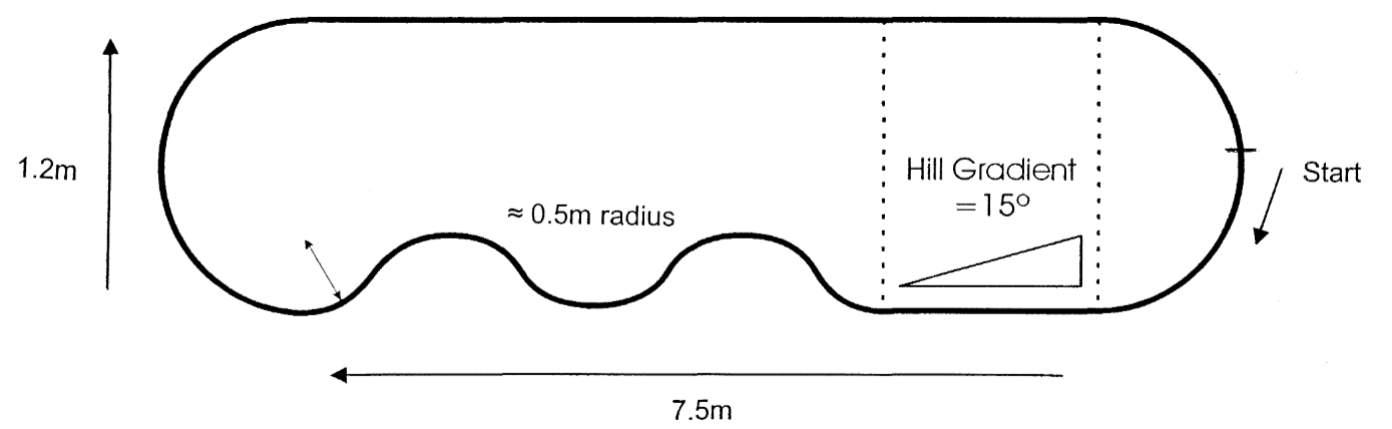
\includegraphics[width=0.9\linewidth]{photos/test_track.png}
    \caption[Mouse Track Geometry]{`mouse' test track geometry taken from \cite{Robinson2025}}
    \label{fig:testtrack}
\end{figure}

\begin{figure}[H]
    \centering
    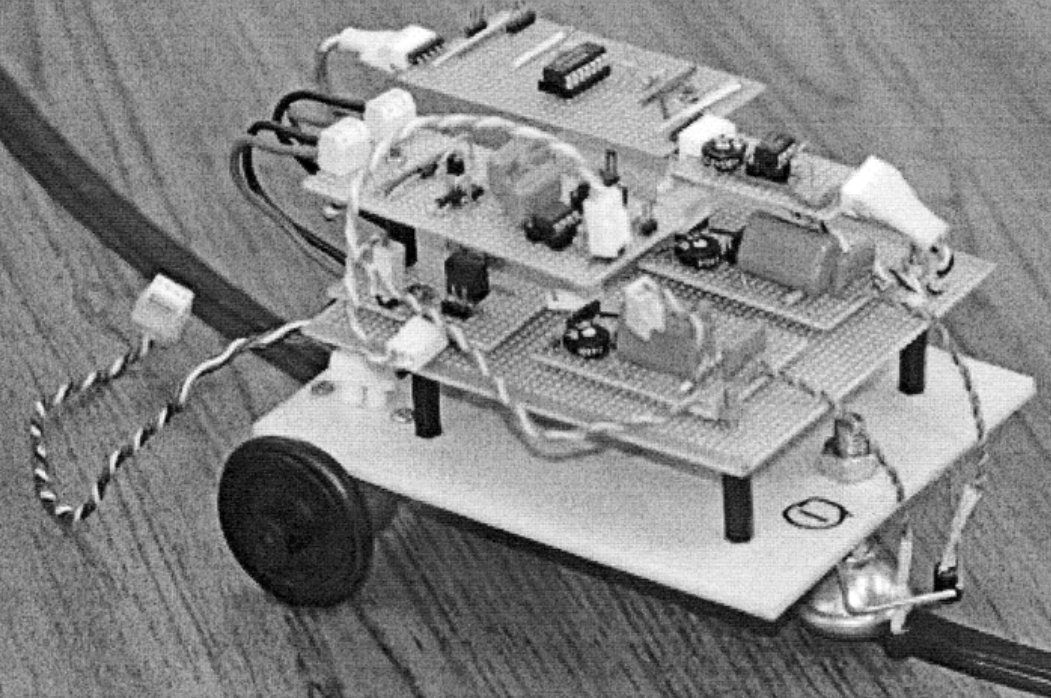
\includegraphics[width=0.6\linewidth]{photos/mouse_build.png}
    \caption[Mouse Build]{`mouse' build example taken from \cite{Robinson2025}}
    \label{fig:mouse}
\end{figure}

\newpage
The initial concepts used to design the `mouse' in the second year are described in Dr Robinson's initial document outlining the project \cite{Robinson2025}. A list of basic `mouse' building blocks can be seen below, and their integration with one another in Fig.\ref{fig:sysdiagram}.

\begin{itemize}
    \item LC filter circuit tuned to 20 kHz.
    \item Signal amplifier circuit.
    \item Peak detector.
    \item Arduino microcontroller, takes the input signal and conducts PID control to produce an output drive signal for the motors.
    \item Motor drive circuit, utilising transistors acting as switches to allow the low-power Arduino to drive the high-power motor load.
\end{itemize}

\begin{figure}[H]
    \centering
    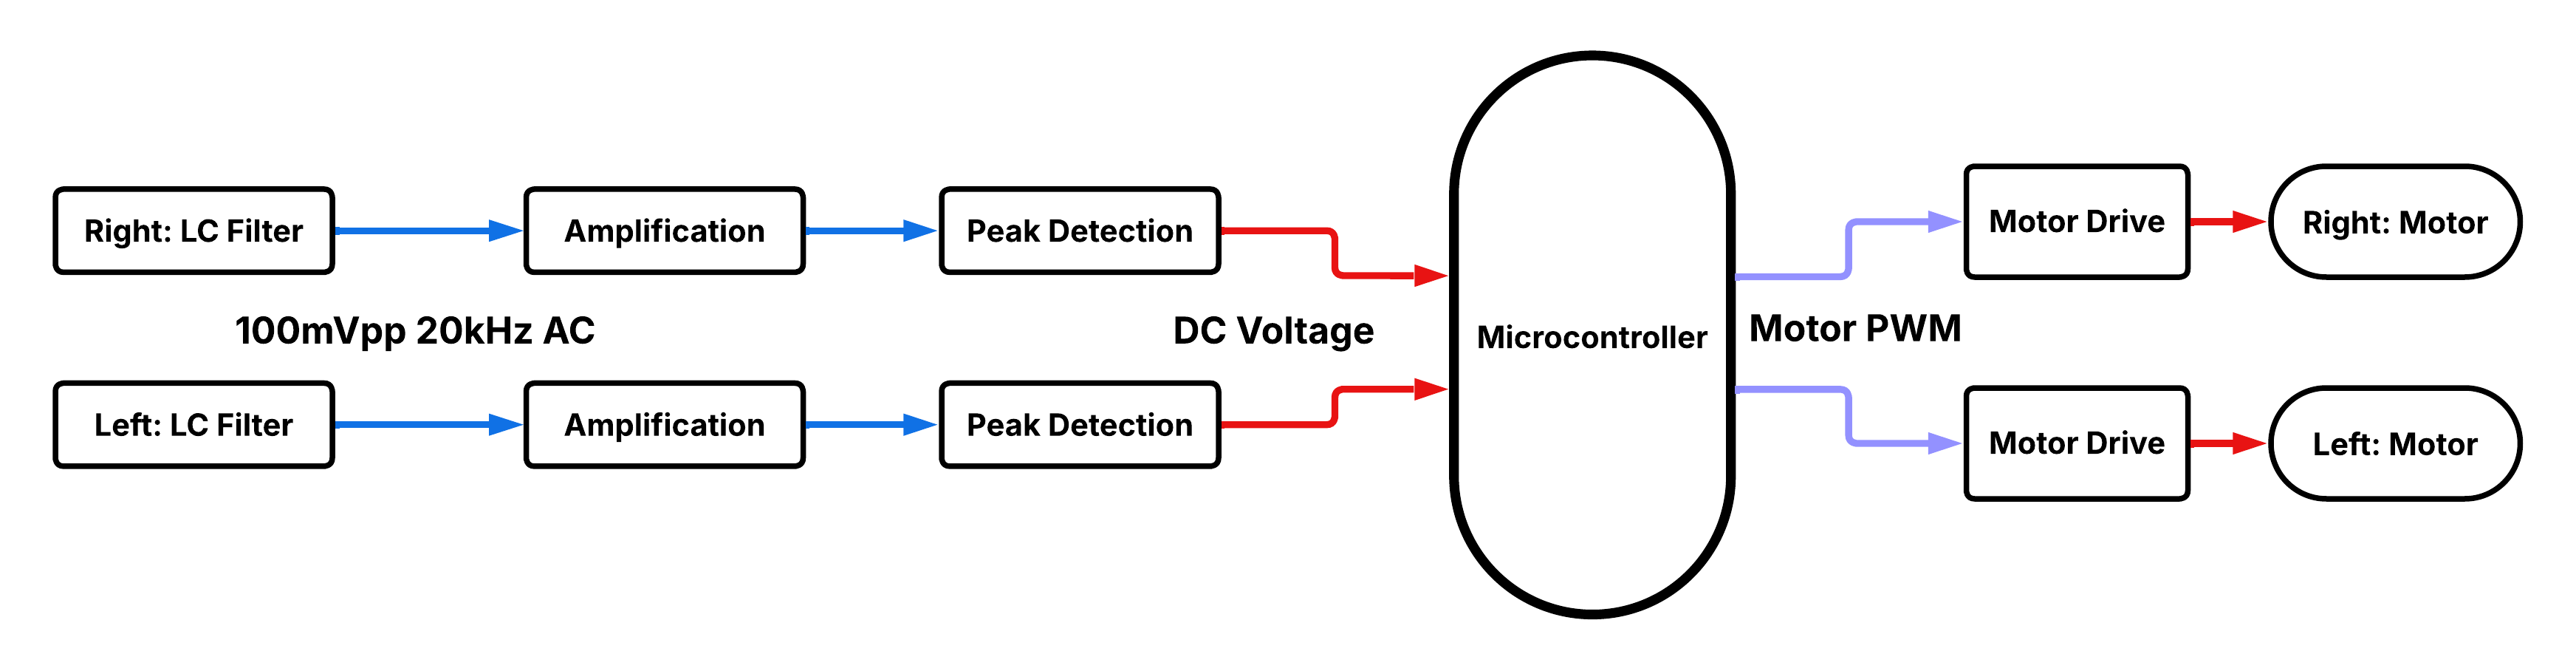
\includegraphics[width=1\linewidth]{photos/sytem diagram original.png}
    \caption[Original `mouse' System Diagram]{Original `mouse' system diagram: Blue, AC Signals; Red, DC Voltages; Purple, Digital Control Signals}
    \label{fig:sysdiagram}
\end{figure}

\subsection{Aims and Objectives}
\label{sec:aims&obj}
As previously outlined in \cite{Noah2025}, the project has three main aims with varying objectives associated with them:
\begin{enumerate}
    \item {Introduce additional stable and accurate feedback loops to the `mouse' control loop, focusing on the lack of feedback from the motors.
    \begin{itemize}
        \item Motor current.
        \item Motor speed.
    \end{itemize}}
    \item {Design alterations and suggestions for the `mouse' that are low-cost and straightforward to integrate.
    \begin{itemize}
        \item Designs should be simple to integrate into a `mouse' project and documentation be available in textbooks or data sheets to assist students if the design is harder to implement. 
        \item Component choice to be limited to low-cost components/modules, keeping a low-cost per `mouse'. Sub-system changes will ideally keep the cost within \(+25\%\) of the original cost.
    \end{itemize}}
    \item {Investigate the power supply options for the mouse, identifying methods for reducing power supply requirements.
    \begin{itemize}
        \item The number of battery packs used to power the mouse ideally reduced from 2 x \(9\) V PP3 alkaline batteries and 4 x \(1.2\) V NiMH AA batteries.
    \end{itemize}}
\end{enumerate}

\subsection{Constraints}
The constraints of this project follow those set out in \cite{Robinson2025}, with an additional self-imposed constraint of not increasing the sub-system cost by over \(25\%\) when compared to current sub-systems.

\section{Initial Ideas Regarding Implementation}
\begin{itemize}
    \item To reduce consumables, weight, and improve environmental impact by removing one of the \break \(9\) V alkaline batteries.
    \item To improve the motor control loop by adding motor current and wheel speed as additional feedback parameters. Potential new system diagram as shown in Fig.\ref{fig:completesys_block}.
\end{itemize}

\begin{figure}[H]
    \centering
    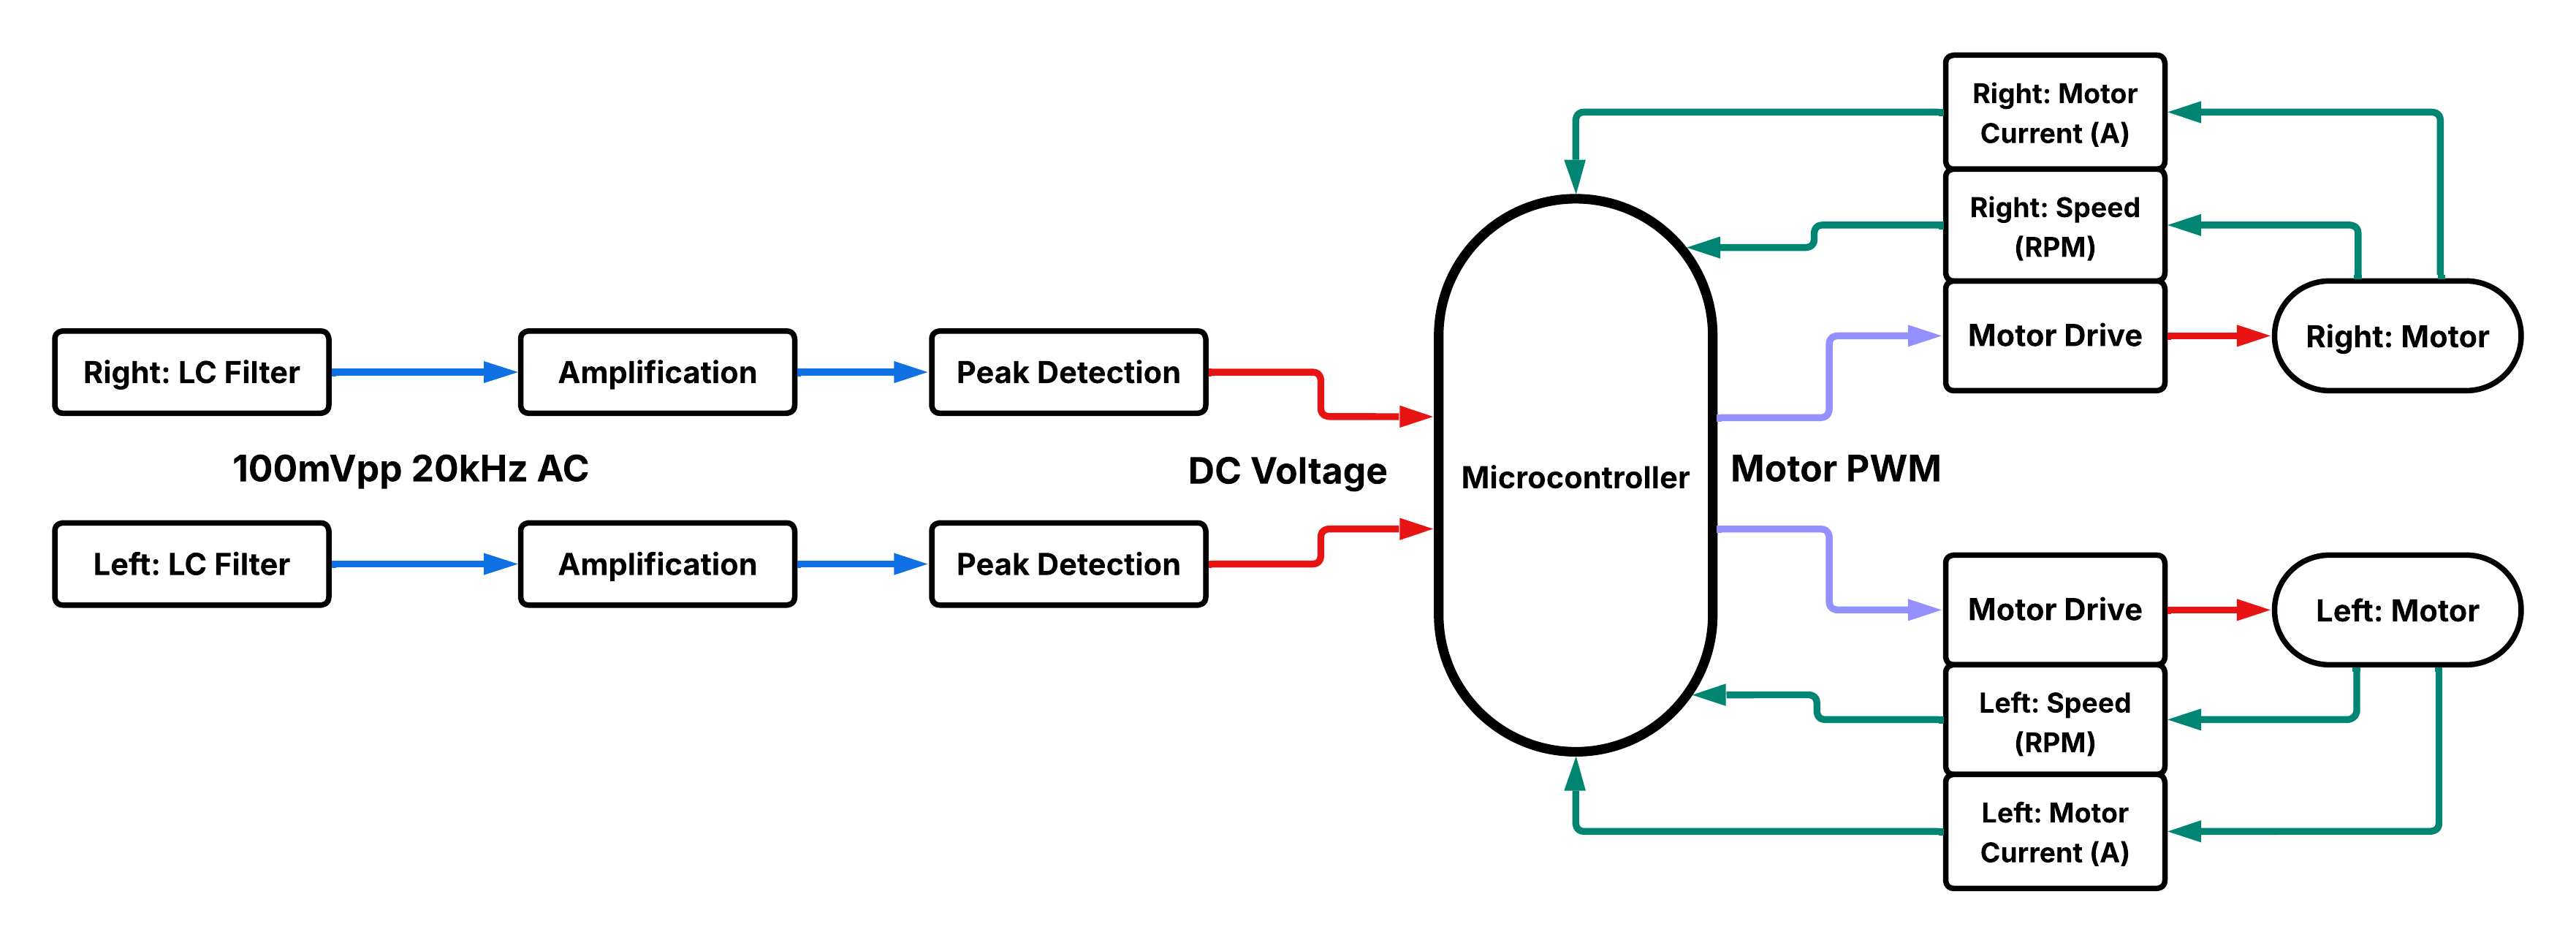
\includegraphics[width=1\linewidth]{photos/sytem diagram.png}
    \caption[Updated `mouse' System Block Diagram]{Updated `mouse' system diagram: Blue, AC Signals; Red, DC Voltages; Purple, Digital Control Signals; Teal, Additional Feedback}
    \label{fig:completesys_block}
\end{figure}


\begin{table}[H]
    \centering
    \caption{Sub-Project Letter Assignments}
    \begin{tabular}{|c|l|l|} \hline 
         \textbf{Design Letter}&   \textbf{Sub-Project Name}&\textbf{Sub-system}\\ \hline  \hline 
 \hyperref[sec:volt_div]{A}& Voltage Divider&  Position Feeedback\\ \hline
 \hyperref[sec:2]{B}& 555 Timer&Position Feeedback\\\hline
 \hyperref[sec:3]{C}& Precision Diode Clamper&Position Feeedback\\ \hline \hline 
 \hyperref[sec:4]{D}& Hall Effect Sensor&Speed Feeedback\\\hline
 \hyperref[sec:5]{E}& IR Optical Sensor&Speed Feeedback\\\hline\hline
 \hyperref[sec:6]{F}& Low Side Motor Drive&Current Feedback\\\hline
 \hyperref[sec:7]{G}& High Side Motor Drive&Current Feedback\\\hline\end{tabular}
    \label{tab:letterciruit_def}
\end{table}

Table \ref{tab:letterciruit_def} lists the sub-projects and the letters assigned for quick reference, including the relevant affected sub-systems.

\subsection{Results Gathering}
All testing procedures and methods list the equipment used, photographed in Appendix \ref{app:equip&test}.




\chapter{Position Feedback}
\section{Overview}
This section discusses the position feedback sub-system of the autonomous `mouse'. The position feedback within the `mouse' control loop is responsible for detecting the mouse's approximate location in relation to the track wire and providing a position feedback signal for steering correction. The current circuit design utilises inductive pick-up coils to sense the AC magnetic flux generated by a trackwire conducting at \(20\) kHz \(\simeq1\) A. The induced voltage signal is subsequently processed by filtering, amplification and peak detector stages to produce a DC feedback signal \cite{Robinson2025}.

A key focus of this section is to address one of the limitations identified in the original sensing sub-system design: the requirement for a dual power supply to bias the operational amplifier appropriately to process a \(100\) mVpp AC signal. This dependency increases the number of batteries required, increasing the `mouse' weight and the project's environmental impact by increasing e-waste. This section aims to explore and implement alternative circuit configurations capable of operating from a single supply of \(9\) V DC. The proposed solutions must maintain signal integrity and compatibility with downstream control systems. The designs must be evaluated on performance, simplicity, and cost of implementation.

\section{Design Concepts and Methods}

\subsection{Design A: Voltage Divider}
Design A (Fig.\ref{fig:vol_div_theory}) employs a voltage divider to proportionally split the \(9\) V input supply voltage to create a new virtual GND. The division is done across two or more resistive sources (see Fig.\ref{fig:vol_div_theory}) with the output voltage dependent on the ratio between the component's impedances. The resulting output voltage equation (Eq.\ref{equ:vol_div}) is derived using Kirchhoff's Voltage Law and Ohm's Law, where \(Z_1\) and \(Z_2\) are impedances of the two components shown in Fig.\ref{fig:vol_div_theory}. The impedance ratio in Design A is set at \(1:1\) resulting in a \(4.5\) V virtual GND

\begin{equation}
    V_{Out}=\frac{Z_2}{Z_1+Z_2}*V_s
    \label{equ:vol_div}
\end{equation}

\begin{figure}[H]
    \centering
    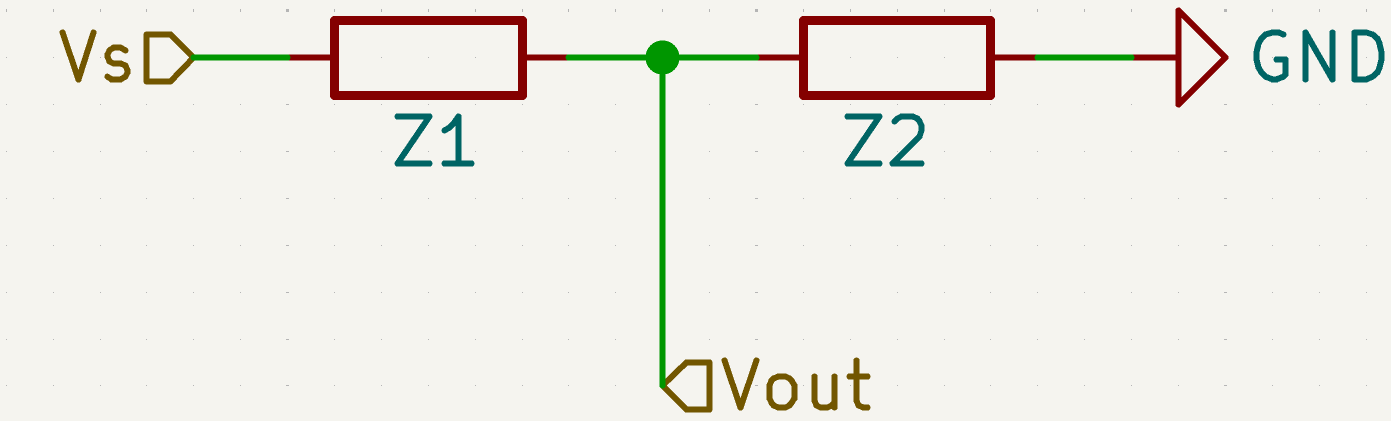
\includegraphics[width=0.7\textwidth]{circuits/volt_div.png}
    \caption[Simple Voltage Divider]{Voltage divider circuit with two resistive components, \(V_s\) is the supply voltage and \(V_{out}\) is the reduced voltage reference.}
    \label{fig:vol_div_theory}
\end{figure}

The new \(4.5\) V virtual GND becomes the new reference point for the operational amplifier and input signal. The operational amplifier and input signal will treat the \(4.5\) V reference as its GND. Biasing the operational amplifier and input signal this way allows the supply rails to be at \(9\) V (\(+ve\) supply) and \(0\) V (\(-ve\) supply), and allows for the use of a single power supply, however the operational amplifier is now operated with a \(\pm4.5\) V supply halving amplification potential. Therefore, an AC-coupled input signal will not reduce the inputs below the \(-ve \) supply rail and cause the operational amplifier to malfunction.

\subsection{Design B: 555 Timer with Negative Charge Pump}
Design B (Fig.\ref{fig:555_ti}) utilises a 555 timer circuit in an astable configuration to generate a rectangular wave output, which drives a negative charge pump circuit. This arrangement allows the generation of a negative voltage supply from a single positive \(9\) V voltage source.

\subsubsection{Astable 555 Timer Operation}

The 555 timer's oscillation frequency is determined by the values of two resistors (\(R_a\) and \(R_b\)) and one capacitor (\(C\)) as shown in Fig.\ref{fig:555_ti}. The resulting output is a square wave with frequency calculated using Eq.\ref{equ:555_frq} as defined by Texas Instruments \cite[p.12]{TI_NE555}.
\begin{equation}
    \label{equ:555_frq}
    f =\frac{1.44}{(R_a+2R_{b})*C}
\end{equation}

The duty cycle of the astable output can be calculated using Eq.\ref{equ:555_duty} as defined by Texas Instruments \cite[p.12]{TI_NE555}.

\begin{equation}
    \label{equ:555_duty}
    Duty =\frac{R_a+R_{b}}{R_a+2R_{b}}*100\%
\end{equation}

\begin{figure}[H]
    \centering
    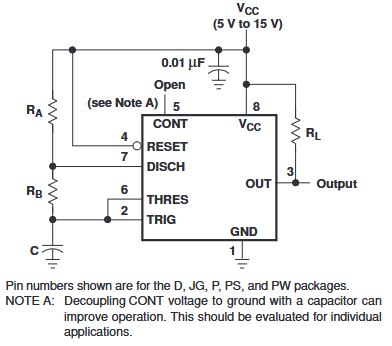
\includegraphics[width=0.7\textwidth]{circuits/555_TI.png}
    \caption[Astable 555 Timer Circuit]{Astable 555 timer circuit configuration showing component connections and pin assignments \cite[p.12]{TI_NE555}. The circuit illustrates the standard configuration for generating rectangular wave outputs with frequency determined by \(R_A\), \(R_B\), and \(C\) values.}
    \label{fig:555_ti}
\end{figure}

\subsubsection{Negative Charge Pump Circuit}
The negative charge pump takes the oscillating output from the 555 timer and converts it to a negative DC voltage through a network of capacitors and diodes (Fig.\ref{fig:negcharge_theo}) as described by Horowitz and Hill \cite[pp.638-639]{Horowitz_Hill_AoE}.

The circuit operates by alternately charging and discharging capacitors through the diodes following the input waveform transitions. When the input signal (\(V_s\)) transitions to a high state, capacitor C1 charges through diode D2 towards GND. Diode D1 remains reverse-biased in this state, preventing current flow towards the output stage. As \(V_s\) switches to a low state, the voltage at the left side of C1 falls below GND potential. This voltage shift forward-biases diode D1, allowing charge to transfer to capacitor C2, which stores the accumulated negative voltage.

During each subsequent cycle of \(V_s\), the additional charge is transferred to C2, gradually increasing the magnitude of the negative output voltage at \(V_{neg}\). Diode D2 prevents the backflow of current during the low phase of \(V_s\), ensuring efficient charge transfer in one direction. The steady-state negative voltage developed across C2 depends on the amplitude of \(V_s\), the capacitance values of C1 and C2, the forward voltage drops of D1 and D2, and the switching frequency of the input signal.

\begin{figure}[H]
    \centering
    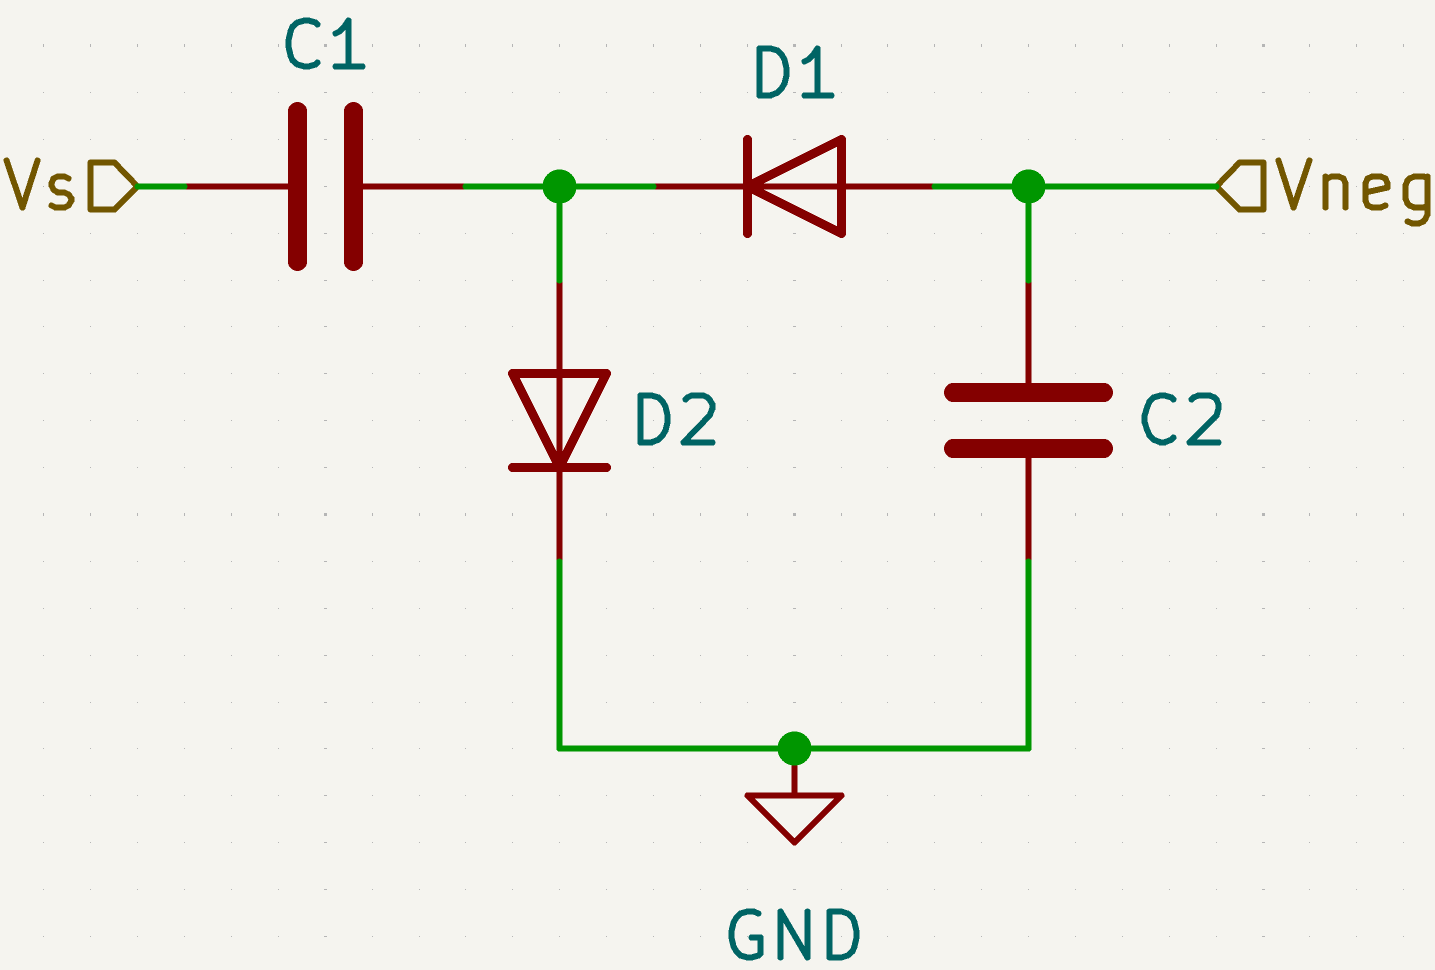
\includegraphics[width=0.6\textwidth]{circuits/neg_charge.png}
    \caption[Negative Charge Pump Circuit]{Schematic of a negative charge pump circuit using a pair of diodes and two capacitors. The circuit generates a negative output voltage (\(V_{neg}\)) from a positive square wave input (\(V_s\)) by transferring charge through C1 and rectifying the output via D1 and D2. Capacitor C2 acts as an output reservoir, smoothing the generated negative voltage.}
    \label{fig:negcharge_theo}
\end{figure}

The voltage efficiency of the charge pump under load can be defined as shown in Eq.\ref{eq:efficincee} where \(V_{neg}\) is the output voltage and \(Vs\) is the supply voltage.

\begin{equation}
\label{eq:efficincee}
    \eta=\frac{-(V_{neg})}{V_s}
\end{equation}

The negative charge pump creates a virtual negative voltage rail relative to the system GND. This new virtual negative rail and the \(9\) V power supply are used as the power rails for an operational amplifier. This setup allows the operational amplifier to have a dual supply from a single positive power supply, enabling regular signal processing operation.

\subsection{Design C: Precision Diode Clamping}
\begin{figure}[H]
    \centering
    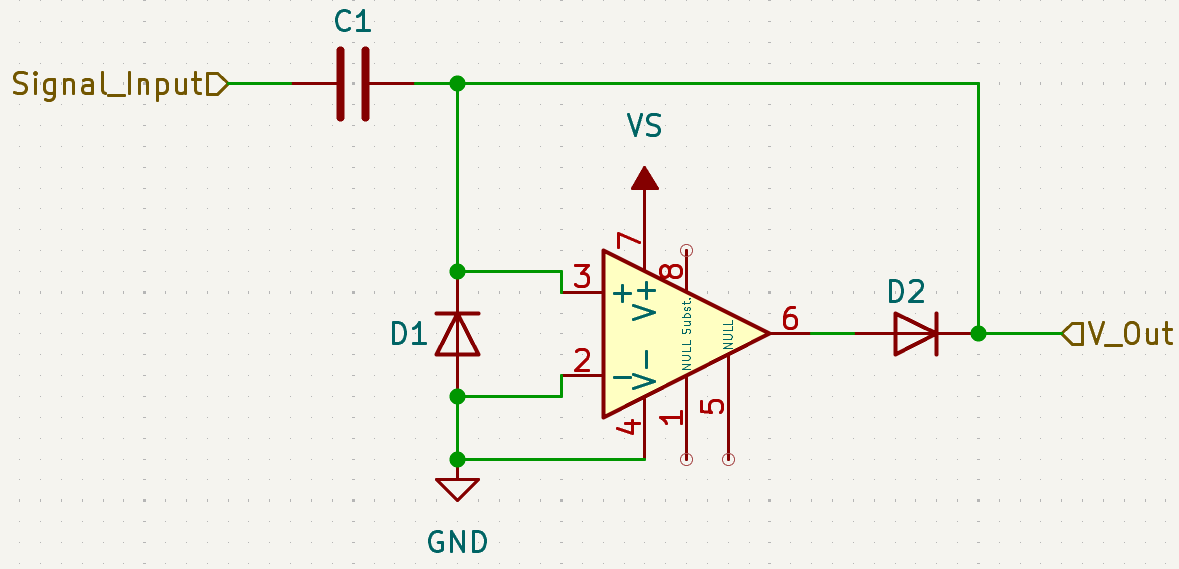
\includegraphics[width=0.8\textwidth]{circuits/prec_diode_clamp.png}
    \caption[Precision Diode Clamper Circuit]{Schematic of a precision diode clamper.}
    \label{fig:precidiode_clamp}
\end{figure}

Design C utilised a precision diode clamping circuit (Fig.\ref{fig:precidiode_clamp}) to clamp the voltage level of the input signal above \(0\) V and hence above GND. When the `Signal\_Input' drops below zero, the diode becomes forward-bias and allows current to pass, causing the capacitor to charge to the voltage level of the negative peak. The diode switches off once the input voltage rises back into the positive range, preventing further current flow. The charged capacitor then effectively adds its stored voltage to the input signal, shifting the entire waveform upward. As a result, the negative portions of the signal are raised closer to zero volts or higher. By pulling the signal above \(0\) V the signal can be amplified by an operational amplifier with supply rails at \(9\) V (\(+ve\) supply) and \(0\) V (\(-ve\) supply) allowing for the use of a single power supply. The effectiveness of this method depends on the characteristics of the operational amplifier used.


\section{Procedures}
\subsection{Design A: Voltage Divider}
\label{sec:volt_div}
\subsubsection{Assembly}

\begin{figure}[H]
    \centering
    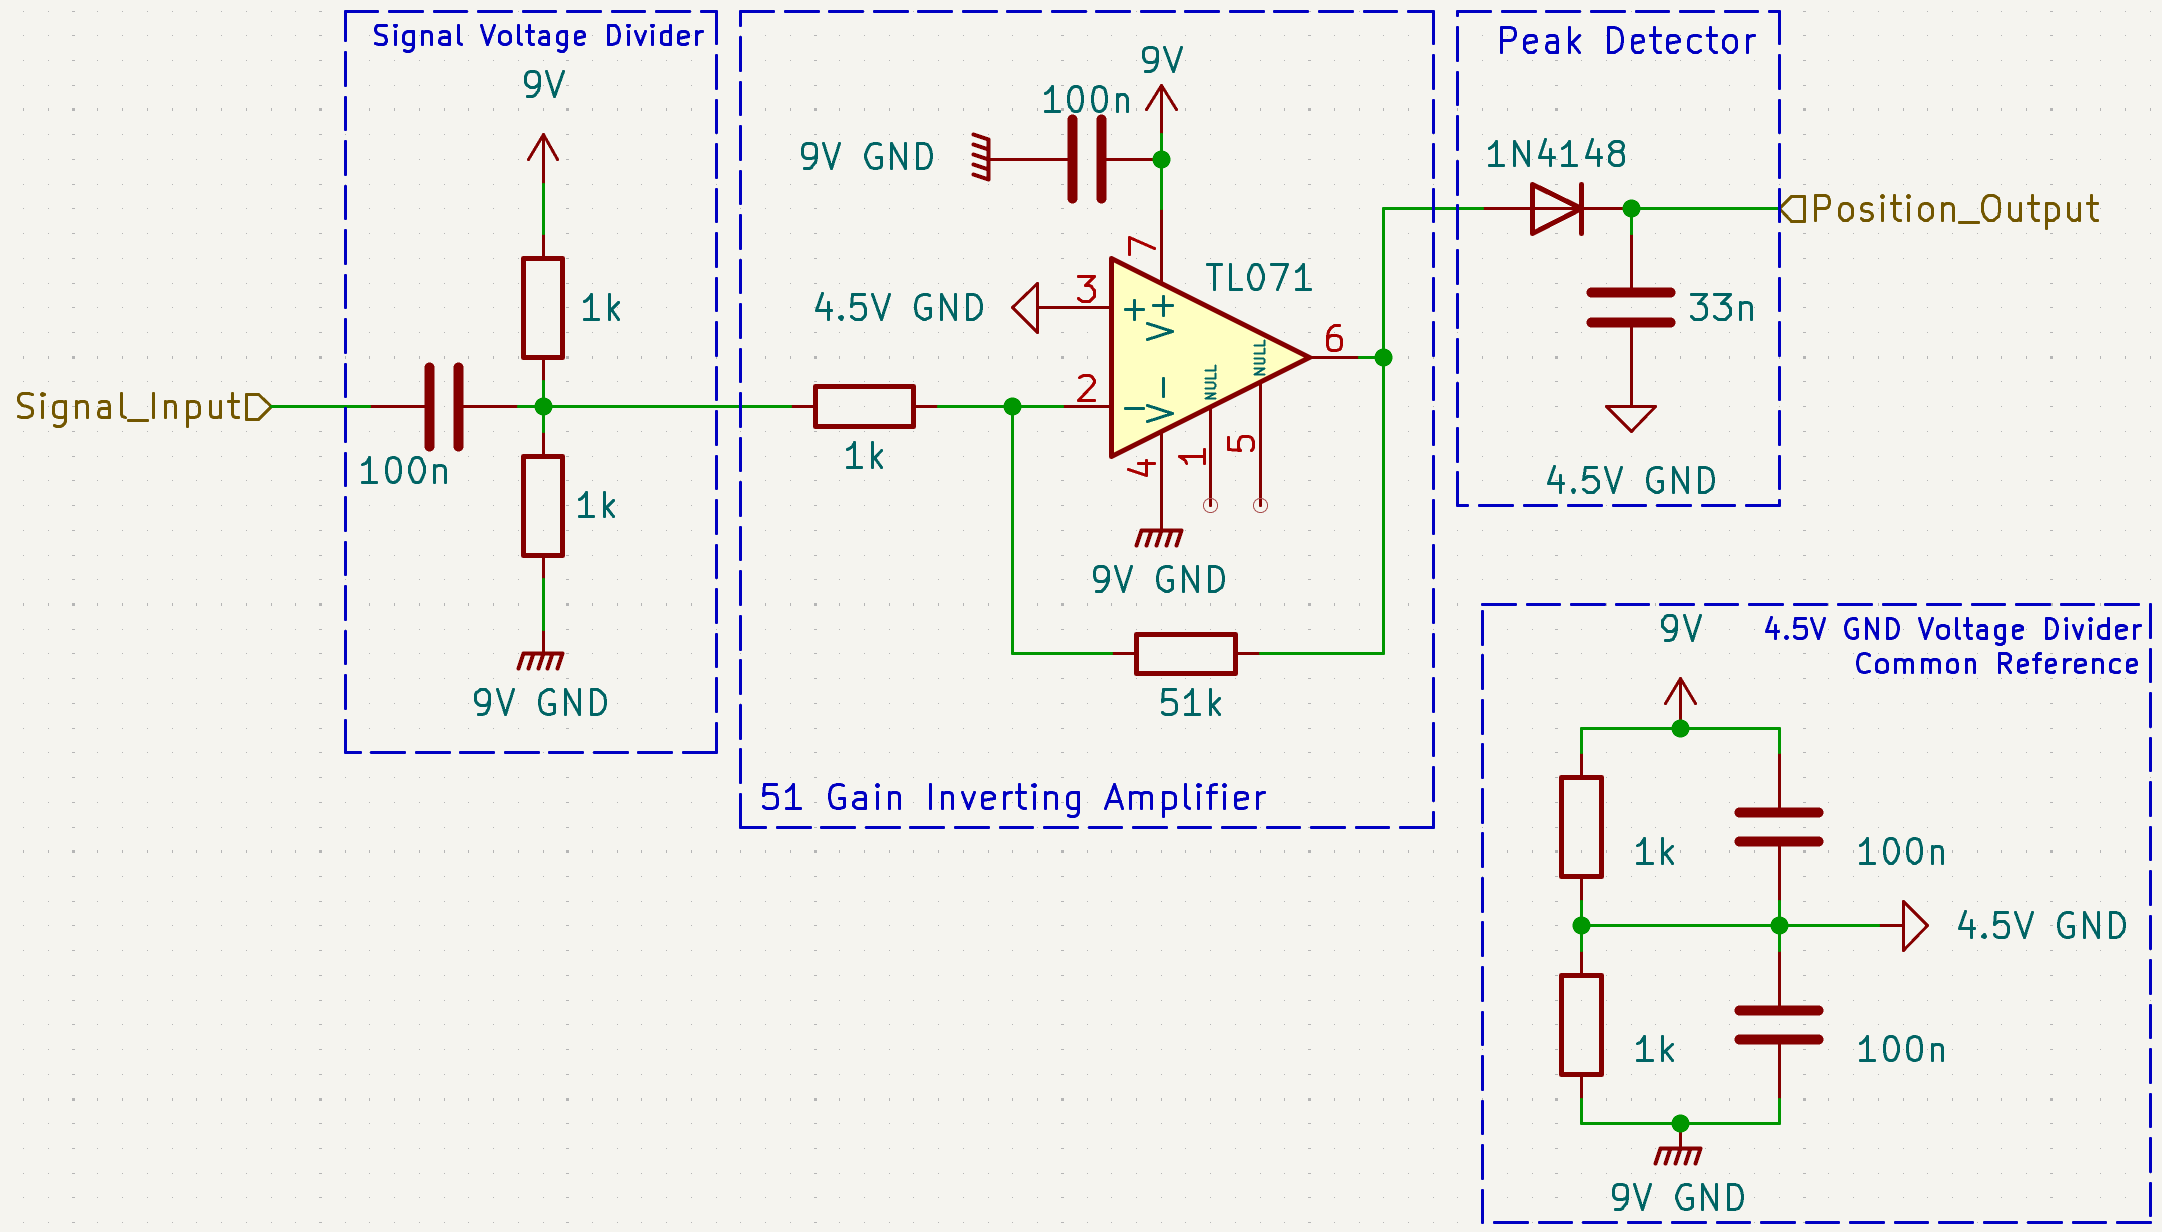
\includegraphics[width=1\linewidth]{circuits/volt_div_possub.png}
    \caption[Design A: Schematic]{Schematic of Design A. Including a voltage divider signal conditioning circuit with a 4.5 V virtual GND, ×51 inverting amplifier, and peak detector, powered from a single 9 V DC supply.}
    \label{fig:vol_div_circuit}
\end{figure}

Design A was built on a standard RH-32 breadboard following the design outline in Fig.\ref{fig:vol_div_circuit}. Firstly, the TL071 \cite{TI_TL071} operational amplifier was inserted into the breadboard and was configured in an inverting arrangement with a gain factor (\(A_v\)) of -51 (Eq.\ref{equ:inverting_amp}), the gain was set by the \break \(51\) k\(\Omega\) feedback resistor (\(R_f\)) and \(1\) k\(\Omega\) input resistor (\(R_{in}\)).

\begin{equation}
    \label{equ:inverting_amp}
    A_v = -\frac{R_f}{R_{in}}
\end{equation}

All connections made to the inverting input (pin 2) were as short as possible to reduce parasitic capacitance as suggested by Texas Instruments \cite[p.36]{TI_TL071}. The \(9\) V DC E3631A lab power supply was connected to pin 7 (\(+ve\) supply rail) with a \(100\) nF decoupling capacitor. The 9 V GND was then connected to pin 4 (\(-ve\) supply rail).

Secondly, a voltage divider circuit was constructed to create the \(4.5\) V GND (virtual GND). As shown in Fig.\ref{fig:vol_div_circuit} two \(1\) k\(\Omega\) resistors were connected in parallel with two \(100\) nF capacitors, the input of the voltage divider was connected to the  \(9\) V DC E3631A lab power supply and the \(9\) V GND was connected to the bottom. The output \(4.5\) V virtual GND was then taken from the central connection as seen in Fig.\ref{fig:vol_div_circuit}. The new \(4.5\) V virtual GND was then connected to the non-inverting input of the TL071.

Third, a voltage divider circuit was constructed to bias the input signal. As shown in Fig.\ref{fig:vol_div_circuit} two \(1\) k\(\Omega\) resistors were connected in series connecting the  \(9\) V DC E3631A lab power supply and the \(9\) V GND. The `Signal\_Input' was then coupled with a \(100\) nF capacitor at the centre point of the resistor and then further connected to the \(1\) k\(\Omega\) resistor (\(R_{in}\)).

Finally, a simple peak detector was assembled after the TL071 using a 1N4148 \cite{Vishay_1N4148} and \(33\) nF capacitor. The peak detector was constructed as shown in Fig.\ref{fig:vol_div_circuit} with the output of the TL071 connecting to the anode of the diode and the GND connection of the capacitor being connected to the \(4.5\) V virtual GND.

\subsubsection{Testing}
The steps for Testing Design A are as follows:

\begin{enumerate}
    \item \(9\) V, \(4.5\) V virtual GND and \(9\) V GND were verified using a KeySight 34450A multimeter.
    \item The Position\_Output DC voltage was measured three times using a KeySight 34450A multimeter when no input signal was applied to check for a potential failure mode, the values were then averaged. 
    \item The AFG2021 signal generator was turned on, set to high impedance and connected to `Signal\_Input' with GND connected the \(4.5\) V virtual GND. Additionally, a filtering capacitor of \(100\) nF was connected between the Signal\_Input and GND to reduce noise, which wouldn't be included in the final design as the signal normally comes from an LC filtered source. The output signal parameters were a Sine Wave set to \(20\) kHz frequency and \(100\) mVpp amplitude.
    \item{
    The KeySight DSO1014A oscilloscope was connected to Design A, making sure the oscilloscope probe ratio matched the input signal ratio and probe points were as close as possible to the measurement point:
    \begin{itemize}
        \item Channel 1: Output of AFG2021 Signal Generator
        \item Channel 2: TL071 pin 6 with probe reference connected to \(4.5\) V Common Reference
        \item Channel 3: `Position\_Output' with probe reference connected to \(4.5\) V Common Reference
    \end{itemize}
    }
    \item The steady-state \(100\) mV waveform was observed and stored on an external USB as a CSV for later analysis in Excel.

    \item The oscilloscope probes were then removed, and the KeySight 34450A multimeter was connected. The positive probe connected to `Position\_Output' and the reference probe to Design A's Common Reference.

    \item The steady-state DC voltage at \(100\) mVpp was recorded three times. The amplitude of the input signal was reduced by \(10\) mVpp and the new steady-state voltage was recorded in Microsoft Excel. This reduction of \(10\) mVpp was repeated till the amplitude reached \(20\) mVpp.
\end{enumerate}

All measurements were taken after a 5-second stabilisation period to minimise transient effects and were conducted at room temperature (approximately 22°C). The oscilloscope output was imported into Excel and used to generate graphs for analysis. The multimeter readings were tabulated and analysed; linear regression was performed to evaluate the system’s gain and linearity.

\subsection{Design B: 555 Timer and Negative Charge Pump}
\label{sec:2}
\subsubsection{Assembly}

\begin{figure}[H]
    \centering
    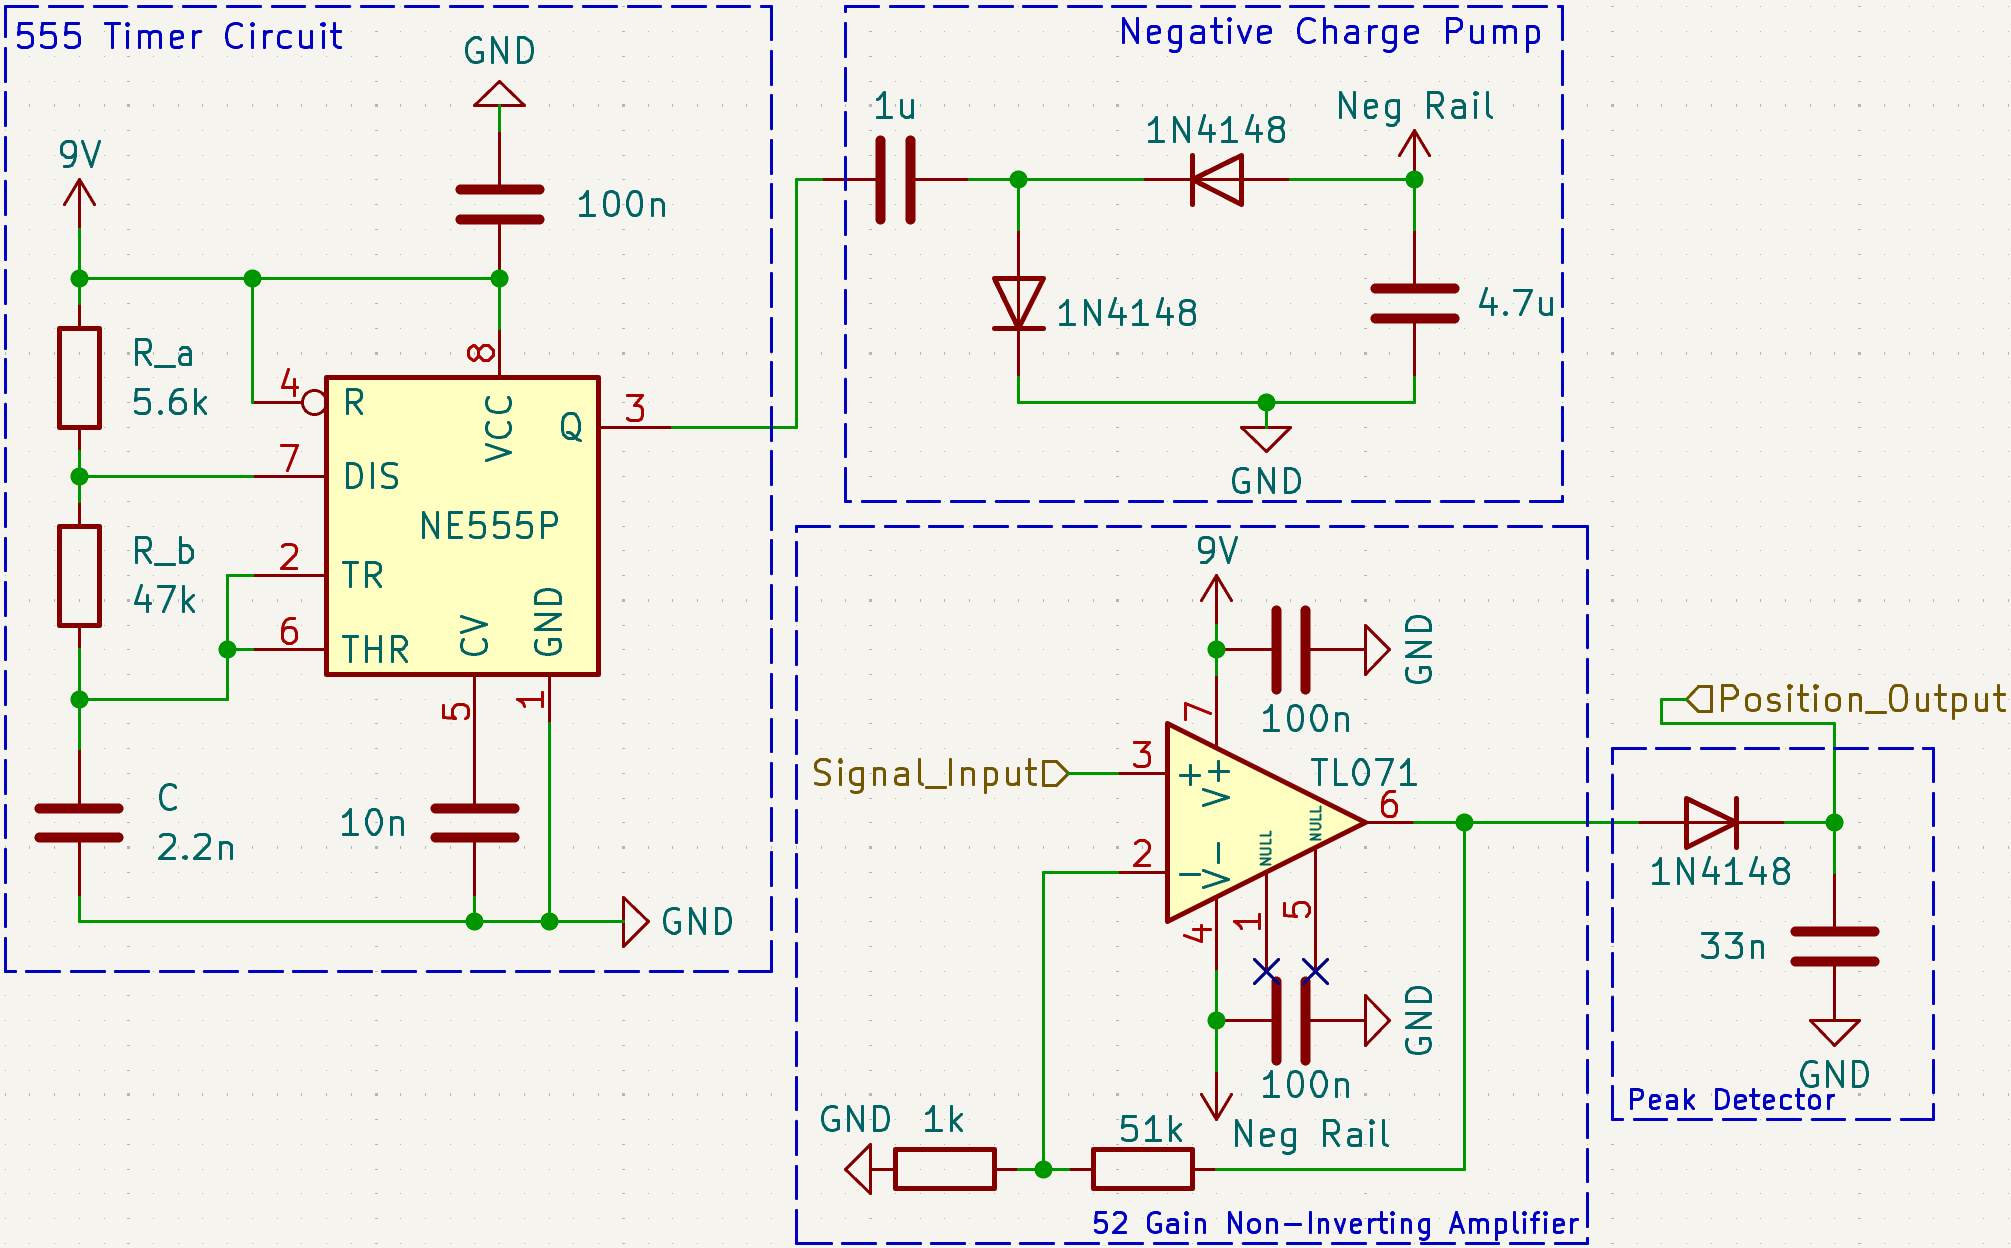
\includegraphics[width=1\linewidth]{circuits/555_possub.png}
    \caption[Design B: Schematic]{Schematic of Design B. Including a 555 astable timer with negative charge pump powered and x52 Non-inverting amplifier, powered from a single 9V DC supply.}
    \label{fig:555_circuit}
\end{figure}

Design B was built on a standard RH-32 breadboard following the design outline in Fig.\ref{fig:555_circuit}. Firstly, the astable mode 555 timer circuit was built using a NE555P \cite{TI_NE555}, the timing components being a \(5.6\) k\(\Omega\) (\(R_a\)), \(47\) k\(\Omega\) (\(R_b\)) and \(1\) nF (\(C\)) as shown in Fig.\ref{fig:555_circuit} following the naming convention used by Texas Instruments \cite[p.12]{TI_NE555}. The timing components selected create an oscillation frequency of \(14.46\) kHz. In addition, a \(10\) nF decoupling capacitor was placed between pin 5 (Control) and GND to improve stability as seen in Fig.\ref{fig:555_circuit} and suggested by Texas Instruments \cite[p.12]{TI_NE555}. Furthermore, during assembly, the timing capacitor and decoupling capacitors were placed as close as possible to the LM555 as advised to reduce possible parasitic capacitance. The \(9\) V DC E3631A lab power supply was connected to pins 4, 8 and the top of \(R_a\); the \(9\) V supply additionally had a \(100\) nF decoupling capacitor. After the 555 timer construction the accompanying negative charge pump circuit was built as seen in Fig.\ref{fig:555_circuit} using two 1N4148 diodes and two capacitors of values \(1\) \(\mu\)F and \(4.6\) \(\mu\)F.

Following on the TL071 operational amplifier \cite{TI_TL071} was inserted into the breadboard and was configured in a non-inverting arrangement with a gain factor (\(A_v\)) of gain factor of 52 (Eq.\ref{equ:noninverting_amp}) the gain was set by the \(51\) k\(\Omega\) feedback resistor(\(R_{f}\)) and \(1\) k\(\Omega\) GND resistor (\(R_{GND}\)). 

\begin{equation}
    \label{equ:noninverting_amp}
    A_v = 1+\frac{R_f}{R_{GND}}
\end{equation}


Again, all connections made to the inverting input (pin 2) were as short as possible, as mentioned in Section \ref{sec:volt_div}. The \(9\) V DC E3631A lab power supply was connected to pin 7 (\(+ve\) supply rail) and the negative charge pump output was connected to pin 4 (\(-ve\) supply rail); both supply rails had \(100\) nF decoupling capacitors.

\subsubsection{Testing}
Firstly, the DC \(9\) V, negative charge pump supply rail and \(9\) V GND were verified using a KeySight 34450A multimeter. The testing method for Design B followed the same procedure as outlined in Section \ref{sec:volt_div} steps \(2\rightarrow7\). All measurements were taken under the same conditions and analysed accordingly as defined in \ref{sec:volt_div}.

\subsection{Design C: Precision Diode Clamping}
\label{sec:3}
Design C was considered but ultimately not physically tested as the low input voltage range [0,100 mV] could not properly forward bias the input diode and risked pulling the inverting input of the operational amplifier below the available negative rail (\(0\) V). This would have resulted in the TL071 operational amplifier operating outside its recommended input range, potentially compromising circuit performance and reliability.

\section{Results}
\subsection{Design A: Voltage Divider}

\begin{table}[h]
    \centering
    \caption[Design A: Supply and Ground Measurements]{Measured DC \(9\) V supply rail and \(4.5\) V virtual GND relative to circuit GND. The potential difference between the circuit GND and the power supply GND was also recorded.}
    \begin{tabular}{|c|c|}
        \hline
        Measurment Point & Measured 3s.f.(V) \\ \hline\hline
        9 V Supply Rail & 8.99 \\ \hline
        4.5 V Virtual GND & 4.49 \\ \hline
        GND & \(6.68*10^{-4}\) \\ \hline
    \end{tabular}
    \label{tab:voltdiv_verification}
\end{table}

The voltage divider was verified at three key points: 9V Supply Rail, 4.5V Virtual GND and GND, as shown in Table \ref{tab:voltdiv_verification}:
\begin{itemize}
    \item \textbf{DC 9 V input}: The output voltage was measured at \(8.99\) V, showing a negligible deviation from the expected value.
    \item \textbf{4.5 V Virtual GND}: The measured voltage was \(4.49\) V, displaying a minimal difference from the theoretical result.
    \item \textbf{0 V (GND)}: The measured voltage was measured at \(6.68 * 10^{-4}\) V ,  approximating to zero confirming correct operation near GND.
\end{itemize}

As summarised in Table \ref{tab:voltdiv_verification}, these results indicate that the voltage divider functioned as expected. When Design A was tested at a 0Vpp input signal the `Position\_Output' remained stable at \(40\) mV.

\begin{figure}[H]
    \centering
    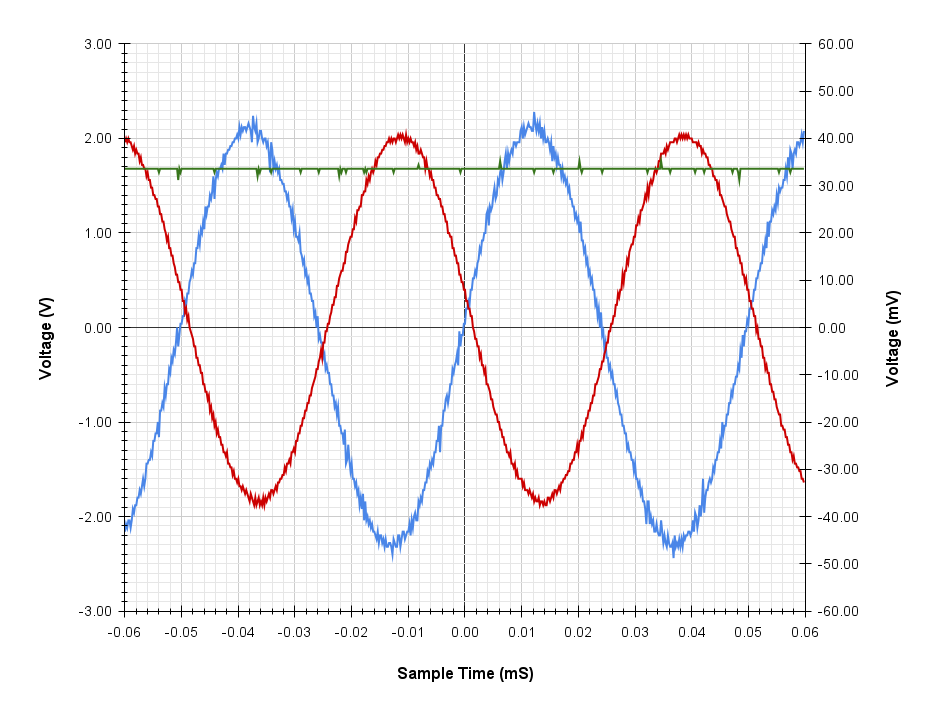
\includegraphics[width=1\linewidth]{graphs/voltagedivider_osciliscope.png}
    \caption[Design A: Oscilloscope Output with input signal of 100mVpp]{Graph showing Design A behaviour at \(100\) mVpp. The traces are the Signal Generator output (Channel 1: Blue), TL071 Operational Amplifier output (Channel 2: Red), and `Position\_Output' (Channel 3: Green) plotted against time (mS). The Signal Generator output is plotted on the right Y-axis in millivolts (mV), while the operational amplifier and Position Output are plotted on the left Y-axis in volts (V).}
    \label{fig:voltdiv_oscilloscope}
\end{figure}

The DSO1014A oscilloscope captured three signals: the `Signal\_Input' (Channel 1), the output of the TL071 operational amplifier (Channel 2), and the `Position\_Output' (Channel 3), as shown in Fig.\ref{fig:voltdiv_oscilloscope}.

\begin{itemize}
    \item \textbf{`Signal\_Input'}: The input sinusoidal waveform with a frequency of \(20\) kHz had peak values ranging from \(-48.8 \) mV to \(45\) mV hence a \(96\) mVpp signal. This indicates a discrepancy in the signal generator output signal and the observed peak-to-peak value.
    \item \textbf{TL071 Output}: The observed output signal inverts the input signal and exhibited peak values of approximately -1.8 V and 2 V, indicating a lower-than-expected gain of \(\approx-42\).
    \item \textbf{`Position\_Output'}: The output of the peak detector shows a steady DC value of approximately 1.7 V. This value is slightly lower than the peak value of the amplified signal (approximately 2 V), due to the voltage drop across the peak detector diode.
    
\end{itemize}

Overall, the oscilloscope graph in Fig.\ref{fig:voltdiv_oscilloscope} confirms that the operational amplifier is amplifying the input signal, though at a lower gain than intended. The peak detector captures a value slightly lower than the peak voltage but still approximately tracks the signal's maximum value.

\begin{figure}[H]
    \centering
    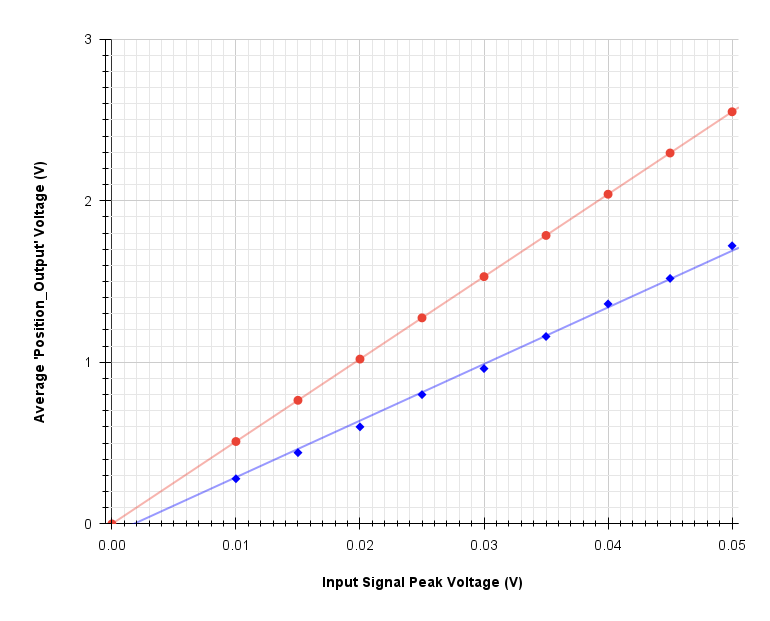
\includegraphics[width=1\linewidth]{graphs/voltagedivider_fullrange.png}
    \caption[Design A: Input Range Response]{Graph of Design A Input Signal Peak Voltage (V) against observed `Position\_Output' (V). Average observed output voltage is represented in Blue, and predicted output voltage is represented in Red.}
    \label{fig:voltdiv_fullrange}
\end{figure}

Fig.\ref{fig:voltdiv_fullrange} demonstrates the relationship between the input peak voltage and the observed output voltage within Design A. As shown in Fig.\ref{fig:voltdiv_fullrange}, the output voltage increases proportionally with the input peak voltage, following a near-linear trend as expected for a fixed-gain inverting amplifier circuit. However, the observed output values were consistently lower than the theoretical values predicted by the amplifier’s nominal gain setting of 51, indicating a reduction in observed gain within the circuit.

The maximum observed voltage was \(1.721\) V and a minimum observed voltage of \(0.280\) V. It should also be noted that the linear trend does not cross through the origin but crosses the x-axis at \(\approx0.002\) V.

These observations confirm the amplifier's overall linear behaviour and highlight the practical limitations demonstrated by the difference between the theoretical gain and the observed gain.

\subsubsection{Cost of Implementation}
\begin{table}[H]
    \centering
    \caption{Alphabetically Ordered Estimated Component Costs for Design A}
    \begin{tabular}{|l|c|c|c|}
    \hline
    \textbf{Component} & \textbf{Quantity} & \textbf{Unit Price (£)} & \textbf{Total Price (£)} \\ \hline\hline
    100nF Ceramic Disc Capacitor (50V) \cite{rs_100nfcap} & 4 & 0.17& 0.68\\ \hline
    1kΩ Resistor \cite{rs_1kresistor} & 5 & 0.162& 0.81\\ \hline
    1N4148 Signal Diode \cite{rs_1n4148} & 1 & 0.01& 0.01\\ \hline
    33nF Capacitor (Polyester, 100V) \cite{rs_33nfcap} & 1 & 0.122& 0.122\\ \hline
    51kΩ Resistor \cite{rs_51kresistor} & 1 & 0.054& 0.054\\ \hline
    9V Battery (RS PRO Alkaline) \cite{rs_9vbattery} & 1 & 2.08& 2.08\\ \hline
    TL071 Op-Amp (Single BiFET) \cite{rs_tl071} & 1 & 0.45& 0.45\\ \hline\hline
    \textbf{Total Estimated Cost} &&&\textbf{£4.21}\\ \hline
    \end{tabular}
    \label{tab:component_info_da}
\end{table}

Table \ref{tab:component_info_da} details the individual components required to implement Design A, alongside their quantities, specifications and unit costs based on UK-sourced pricing at the time of writing. The cost of implementation within the `mouse' would be £5.68, adding an additional inverting amplifier, peak detector and signal voltage divider. The cost difference between the original sub-system (Appendix \ref{app:mouseecost_og}) is -£1.70 a reduction of \(23\%\).

\subsection{Design B: 555 Timer and Negative Charge Pump}
\begin{table}[h]
    \centering
    \caption[Design B: Supply and Ground Measurements]{Measured \(9V\) supply rail and charge pump negative supply rail relative to the circuit GND. The potential difference between circuit GND and E3631A lab power supply GND was also recorded to verify correct internal biasing and GND reference stability within the single-supply configuration.}
    \begin{tabular}{|c|c|}
        \hline
        Measurement Point & Measured 3s.f.(V) \\ \hline\hline
        9 V Supply Rail & 8.99 \\ \hline
        Negative Rail & -5.50 \\ \hline
        GND & \(8.22*10^{-4}\) \\ \hline
    \end{tabular}
    \label{tab:555_verification}
\end{table}

The 555 timer design was verified at three key points: 9 V Supply Rail, Negative Supply Rail, and GND, as shown in Table \ref{tab:555_verification}:
\begin{itemize}
    \item \textbf{9 V input}: The output voltage was measured at \(8.99\) V, showing a negligible deviation from the expected value.
    \item \textbf{Negative Rail}: The measured voltage was \(-5.50\) V, displaying an efficiency of \break \(\frac{-5.50}{9}\approx 61.1\%\). Measured under circuit load.
    \item \textbf{0 V (GND)}: The measured voltage was measured at \(8.22*10^{-4}\) V, approximating to zero confirming correct operation near GND.
\end{itemize}

As summarised in Table \ref{tab:555_verification}, these results indicate that the 555 timer design functioned as expected. In addition, when Design B was tested at a 0Vpp input signal the `Position\_Output' remained stable at \(40\) mV.


\begin{figure}[H]
    \centering
    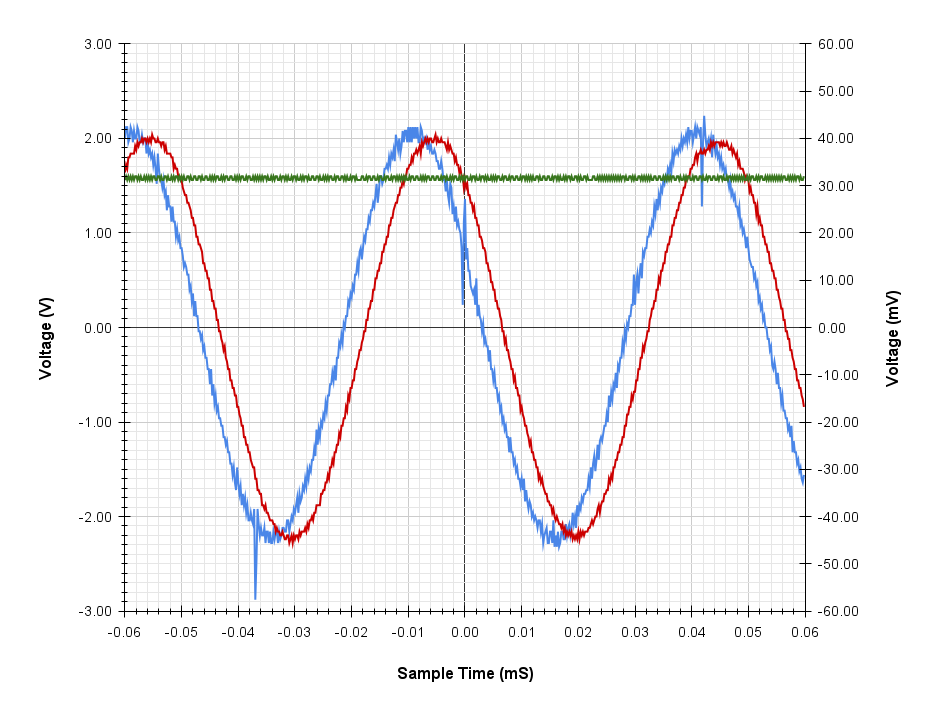
\includegraphics[width=1\linewidth]{graphs/555_osciliscope.png}
    \caption[Design B: Oscilloscope Output with input signal of 100mVpp]{Graph showing Design B behaviour at \(100\) mVpp. The traces are Signal Generator output (Channel 1: Blue), TL071 Operational Amplifier output (Channel 2: Red), and `Position\_Output' (Channel 3: Green) plotted against time (\(mS\)). The Signal Generator output is plotted on the right Y-axis in millivolts (mV), while the operational amplifier and Position Output are plotted on the left Y-axis in volts (\(V\)).}
    \label{fig:555_oscilloscope}
\end{figure}

The DSO1014A oscilloscope captured three signals: the `Signal\_Input' (Channel 1), the output of the TL071 operational amplifier (Channel 2), and the `Position\_Output' (Channel 3), as shown in Fig.\ref{fig:555_oscilloscope}.

\begin{itemize}
    \item \textbf{`Signal\_Input'}: The input sinusoidal waveform with a frequency of \(20\) kHz had peak values ranging from \(-45.6 \) mV to \(42.4 \) mV, \(88\) mVpp signal.
    \item \textbf{TL071 Output}: The observed output signal follows the input signal and exhibited peak values of approximately -2.2 V and 2 V, indicating a lower-than-expected gain of \(\approx45\).
    \item \textbf{`Position\_Output'}: The output of the peak detector shows a steady value of approximately 1.6 V. This value is lower than the peak value of the amplified signal (approximately 2 V), due to the voltage drop across the peak detector diode.
    
\end{itemize}

Overall, the oscilloscope graph in Fig.\ref{fig:555_oscilloscope} confirms that the operational amplifier is amplifying the input signal at a lower gain than intended. The peak detector captures a value lower than the peak voltage but still approximately tracks the signal's maximum value.



\begin{figure}[H]
    \centering
    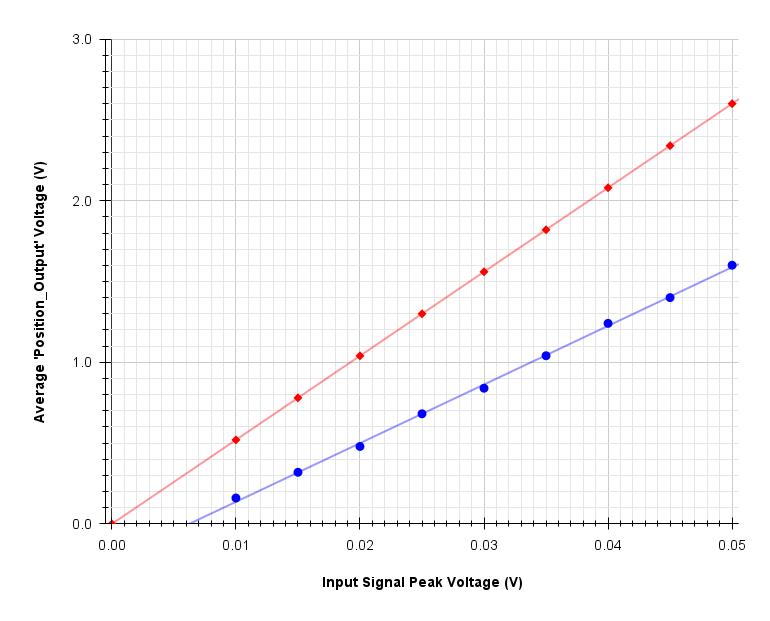
\includegraphics[width=1\linewidth]{graphs/555_fullrange.png}
    \caption[Design B: Input Range Response]{Graph of Design B Input Signal Peak Voltage (V) against observed `Position\_Output' (V). Average observed output voltage is represented in Blue, and predicted output voltage is represented in Red.}
    \label{fig:555_fullrange}
\end{figure}

Fig.\ref{fig:555_fullrange} demonstrates the relationship between the input peak voltage and the observed output voltage within Design B. As shown in Fig.\ref{fig:555_fullrange}, the output voltage increases proportionally with the input peak voltage, following a near-linear trend as expected for a fixed-gain non-inverting amplifier circuit. However, observed output values were consistently lower than the theoretical values predicted by the amplifier’s nominal gain setting of 52, indicating a reduction in observed gain within the circuit.

The maximum observed voltage was \(1.601\) V and a minimum observed voltage of \(0.160\) V. It should be noted that the linear trend does not cross through the origin but crosses the x-axis at \(\approx0.006\) V.

These observations confirm the amplifier's overall linear behaviour, highlighting the practical limitations demonstrated by the difference between the theoretical gain and observed gain.

\subsubsection{Cost of Implementation}

\begin{table}[H]
\centering
\caption{Alphabetically Ordered Estimated Component Costs for Design B}
\begin{tabular}{|l|c|c|c|}
\hline
\textbf{Component}                & \textbf{Quantity} & \textbf{Unit Price (£)} & \textbf{Total Price (£)}\\ \hline
100nF Ceramic Disc Capacitor\cite{rs_100nfcap} & 3 & 0.17 & 0.51\\ \hline
1kΩ Resistor \cite{rs_1kresistor} & 1 & 0.162 & 0.162\\ \hline
1μF Electrolytic Capacitor \cite{rs_1ufcap} & 1 & 0.218 & 0.218\\ \hline
1N4148 Diode \cite{rs_1n4148} & 1 & 0.01 & 0.01\\ \hline
2.2nF Ceramic Capacitor \cite{rs_2nfcap}& 1 & 0.068 & 0.068\\ \hline
33nF Polyester Capacitor  \cite{rs_33nfcap} & 1 & 0.12 & 0.12\\ \hline
4.7μF Electrolytic Capacitor \cite{rs_5ufcap}& 1 & 0.206 & 0.206\\ \hline
47kΩ Resistor \cite{rs_47kresistor}& 1 & 0.167 & 0.167\\ \hline
51kΩ Resistor \cite{rs_51kresistor} & 1 & £0.054 & £0.054\\ \hline
5.6kΩ Resistor \cite{rs_6kresistor}& 1 & 0.106 & 0.106\\ \hline
9V Battery (RS PRO Alkaline) \cite{rs_9vbattery} & 1 & 2.08 & 2.08 \\ \hline
10nF Polyester Capacitor \cite{rs_10nfcap} & 1 & 0.112 & 0.112\\ \hline
NE555P Timer IC \cite{rs_ne555p} & 1 & 0.152 & 0.152\\ \hline
TL071 Operational Amplifier \cite{rs_tl071} & 1 & 0.45 & 0.45\\ \hline\hline
\textbf{Total Estimated Cost} &&&\textbf{£4.41}\\ \hline
\end{tabular}
\label{tab:component_info_db}
\end{table}

Table \ref{tab:component_info_db} details the individual components required for the implementation of Design B, alongside their quantities, specifications, suppliers, and unit costs based on UK-sourced pricing at the time of writing. The cost of implementation within the `mouse' would be £5.54, adding an additional non-inverting amplifier and peak detector. The cost difference between the original sub-system (Appendix \ref{app:mouseecost_og}) is -£1.84 a reduction of \(25\%\). 

\section{Discussion}
This section covered the evaluation of three design solutions proposed to facilitate the operation of the position feedback system from a single DC supply of \(9\) V. Firstly, of the three designs assessed, two designs produced stable outputs when assembled, suggesting these are possible solutions to the dual power supply issue. Secondly, the output signals produced by the physical designs were of an observable voltage level that a microcontroller could utilise for position feedback. Thirdly, the cost of implementation is less than that of the current dual power supply operational amplifier circuit.

Before further interpreting the findings, we must note several important limitations. Firstly, the current methods do not account for varying temperatures. All tests were carried out at room temperature \(22\) \(\degree\)C. Changes in electrical characteristics could cause incorrect design behaviour due to an increase or decrease in device temperatures. This limitation should be considered when shrinking the circuit size down and concentrating components together, increasing potential heat interference from hot components, especially the MOSFETs (IRLZ44N). Secondly, no accommodation is made regarding the observed input signal amplitude and signal generator amplitude discrepancy. This could introduce uncertainty into the observed output DC voltages and the corresponding gain achieved. The primary project aim was to evaluate the linearity and efficacy between designs, rather than obtain absolute voltage values with high precision.  Thirdly, for consistency of results the \(9\) V power rail in Design A and B was provided with a laboratory power supply and not batteries, which will have a higher impedance especially as they discharge with use potentially impacting performance.

\subsubsection{Design Performance}
Design A and B provided consistent and reliable output voltages that linearly followed the input signal voltage. However, the observed `Position\_Output' voltage was lower than the amplifier output due to the voltage drop across the diode; this could be corrected by placing the diode inside the feedback loop. In addition, this would also remove any diode drop with temperature. Furthermore, the observed gain in both designs was lower than expected; however, this shouldn't be an issue in actual application, as variable resistors are used to match the signals, and additional Arduino scaling can be done to balance the left and right sensor signals.

\subsubsection{Complexity}
Design A is simple in background knowledge and requires only basic electrical engineering principles to integrate. In contrast, Design B has more complexity due to introducing difficult principles and complicated circuitry; however, documentation is available to guide the creation of Design B.

\subsubsection{Cost}
Both Design A and B provide a cost reduction from the original sub-system due to the expensive nature of batteries and the removal of one. Comparing the two designs to one another, Design B is slightly more cost-effective with a larger total cost reduction.

\subsubsection{Further Investigations}
Further evaluation should be conducted on Design A and B once integrated into a working `mouse', validating circuit performance with battery supplies and interaction with LC filter circuit. In addition, a set of secondary sensors on the rear of the `mouse' should be investigated, with the intention of using them to help identify straights and corners more effectively.

\subsubsection{Recommendations}
On the whole, both Design A and B are recommended as potential solutions to solve the dual power supply operational amplifier issue. Both designs have valid use cases and should be considered, however in the current state of the `mouse' project Design B is the final recommendation, costing less and having a greater operational range than Design A.






\chapter{Speed Feedback}
\section{Overview}
The primary consideration of this section is developing and evaluating a speed feedback sub-system for the autonomous `mouse'. A limitation of the current `mouse' design is its inability to monitor the RPM of the wheels, meaning the controller cannot adjust the PWM accounting for a sudden reduction or increase in RPM. A typical example of a RPM-related issue is the descent of the track hill. When descending, it is common for the `mouse' to lose control due to a sudden increase in RPM and the controller's inability to account for this. The proposed solutions must provide reliable and responsive RPM readings. The solutions will be evaluated based on the following criteria: stability, simplicity of integration and cost of implementation.

\section{Design Concepts and Methods}
\subsection{Design D: Hall-Effect Sensor}
Design D (Fig.\ref{fig:hes_theory}) utilises a digital hall-effect sensor to detect the presence of a magnet attached to the `mouse' wheel, outputting a signal based on the presence or absence of a magnetic field. Many hall-effect sensors have an open-drain or open-collector output stage, meaning they can pull the output low but not drive it high, for example Allegro A3213 \cite{MicroSystems_2016}. 

\begin{figure}[H]
    \centering
    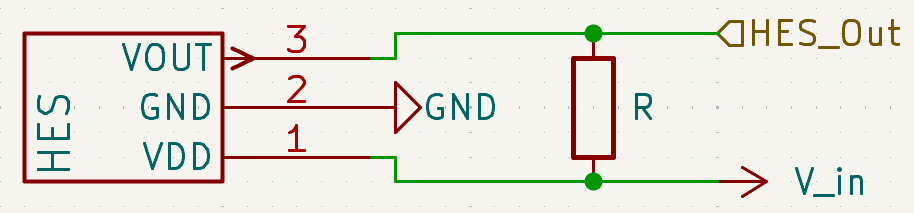
\includegraphics[width=1\textwidth]{circuits/hes_sensor_theory.png}
    \caption[Hall-Effect Sensor with Pull-up Resitor Schematic]{Schematic of a hall-effect sensor circuit with pull-up resistor}
    \label{fig:hes_theory}
\end{figure}

To obtain an observable pulse it is common to use a pull-up resistor between the supply rail and sensor output (Fig.\ref{fig:hes_theory}). This circuit setup results in logic low (0: negative pulse) observed on VOUT when applying a magnetic field and logic high (1: high voltage) when not applying a magnetic field. Typical values for the pull-up resistor (`R') range from \(1\) k\(\Omega\rightarrow50\) k\(\Omega\) depending on required logic levels, speed and current. A smaller `R' value results in a faster response time and an increased current draw when the output is low. A pull-up resistor is critical when interfacing the hall-effect sensor with digital inputs on microcontrollers or logic devices. Without a pull-up resistor, the output may float, resulting in undefined or noisy readings.

\subsection{Design E: IR Optical Sensor}
\begin{figure}[H]
    \centering
    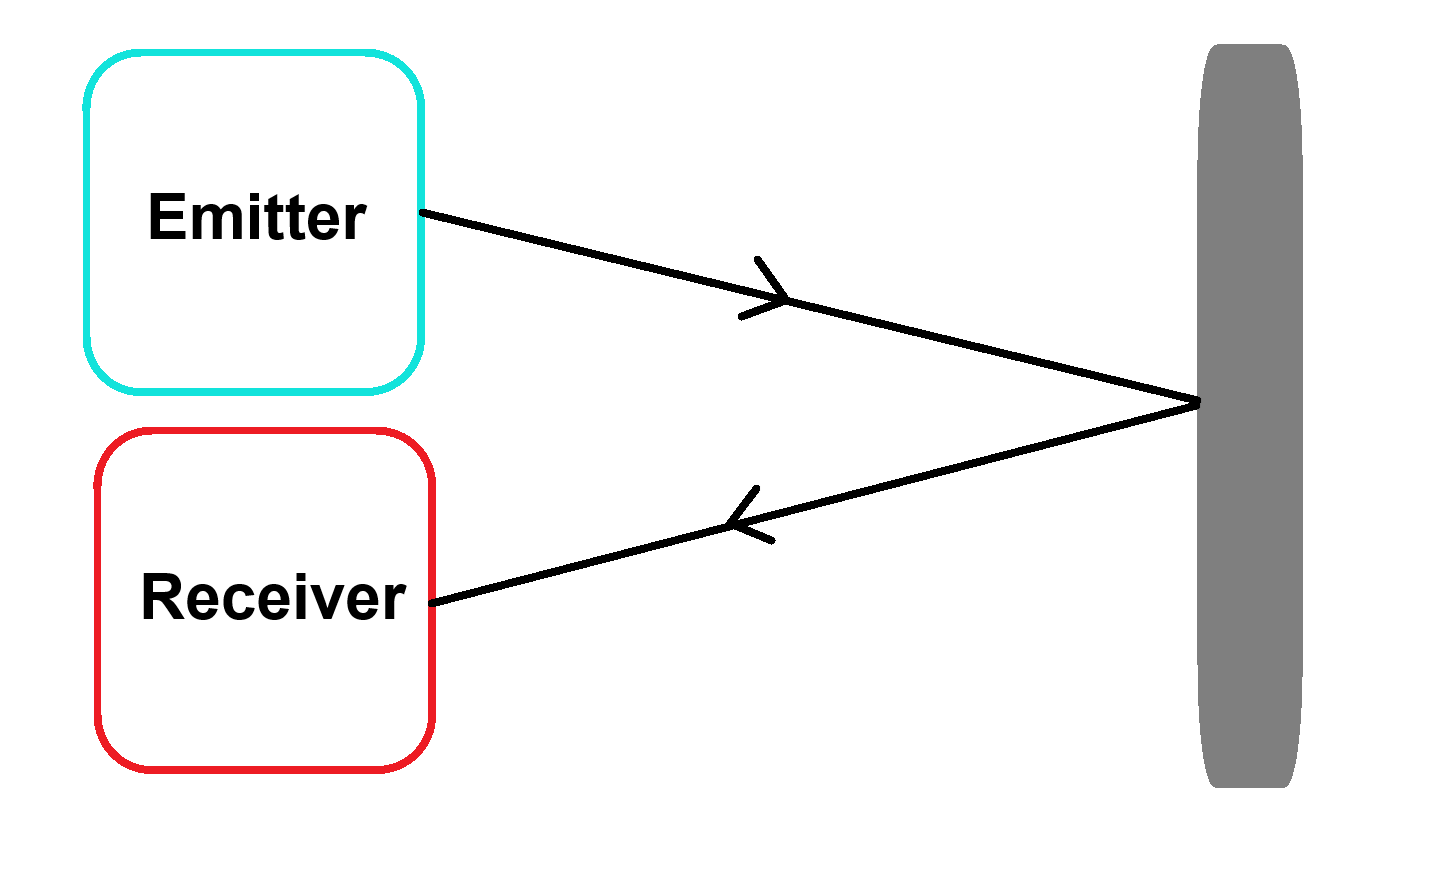
\includegraphics[width=0.6\textwidth]{photos/emitter&receiver.png}
    \caption{Diagram of IR emitter and receiver behaviour}
    \label{fig:opt_theory}
\end{figure}
Design E employs a digital IR emitter and receiver module \cite{Switch_TCRT5000} for detecting the presence of tachometer tape on the `mouse' wheel, outputting a signal based on the presence or absence of IR reflection. The system typically consists of an IR Light Emitting Diode (LED) as the emitter and a phototransistor or photodiode as the receiver. The IR LED emits invisible infrared light toward a target area.

The module utilises a reflective configuration; the emitter and receiver are positioned adjacent facing the target area. When the tachometer tape enters the sensor’s detection zone, it reflects the IR light towards the receiver (Fig.\ref{fig:opt_theory}). The sensor output is then converted from analogue to digital via a comparator or signal conditioning, and the output remains logic low (0: low voltage) when no reflection is detected and switches to logic high (1: high pulse) when a reflection is detected.

\section{Procedures}
Initially, the `mouse' wheel was modified, a \(3\) mm neodymium magnet \cite{RS_2192257} was adhered using hot glue to the outside of the wheel and covered by reflective tachometer tape \cite{RS_8459731} as shown in Fig.\ref{fig:wheel_mag}.

\begin{figure*}[!h]
    \centering
    \begin{subfigure}[t]{0.3\textwidth}
        \centering
        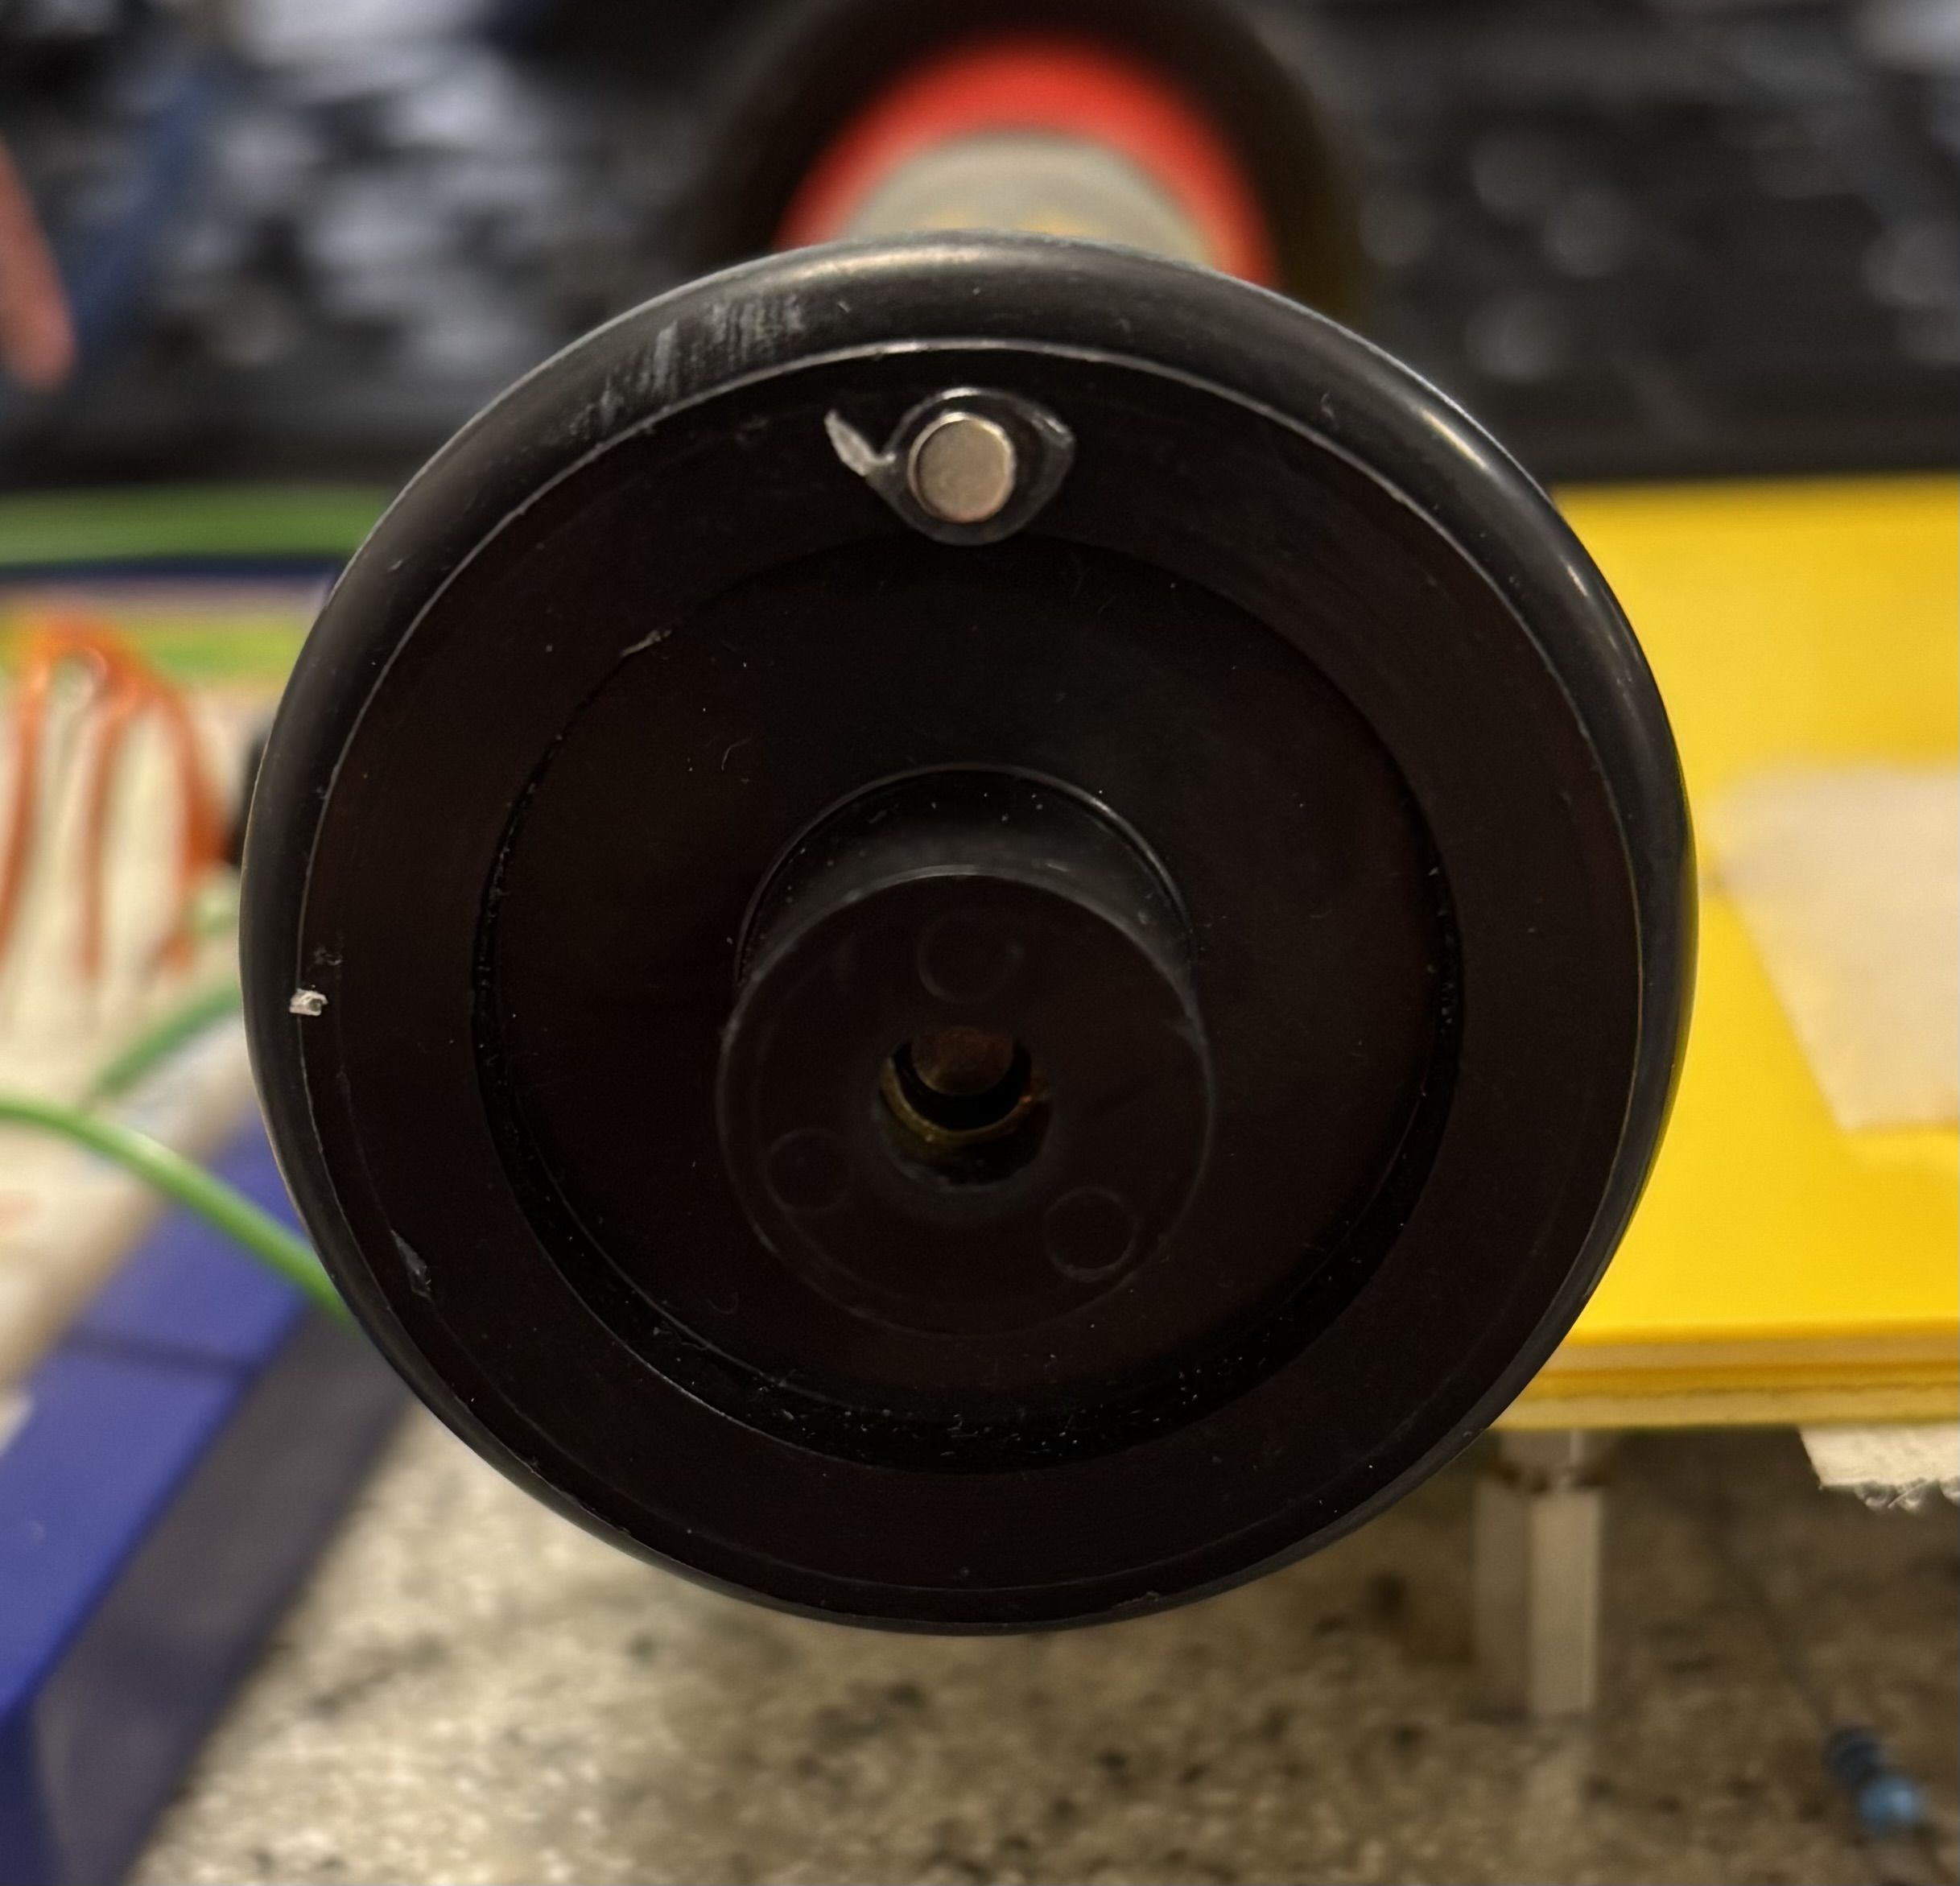
\includegraphics[height=0.8\linewidth]{photos/wheel_2.jpg}
        \caption{}
    \end{subfigure}%
    ~ 
    \begin{subfigure}[t]{0.3\textwidth}
        \centering
        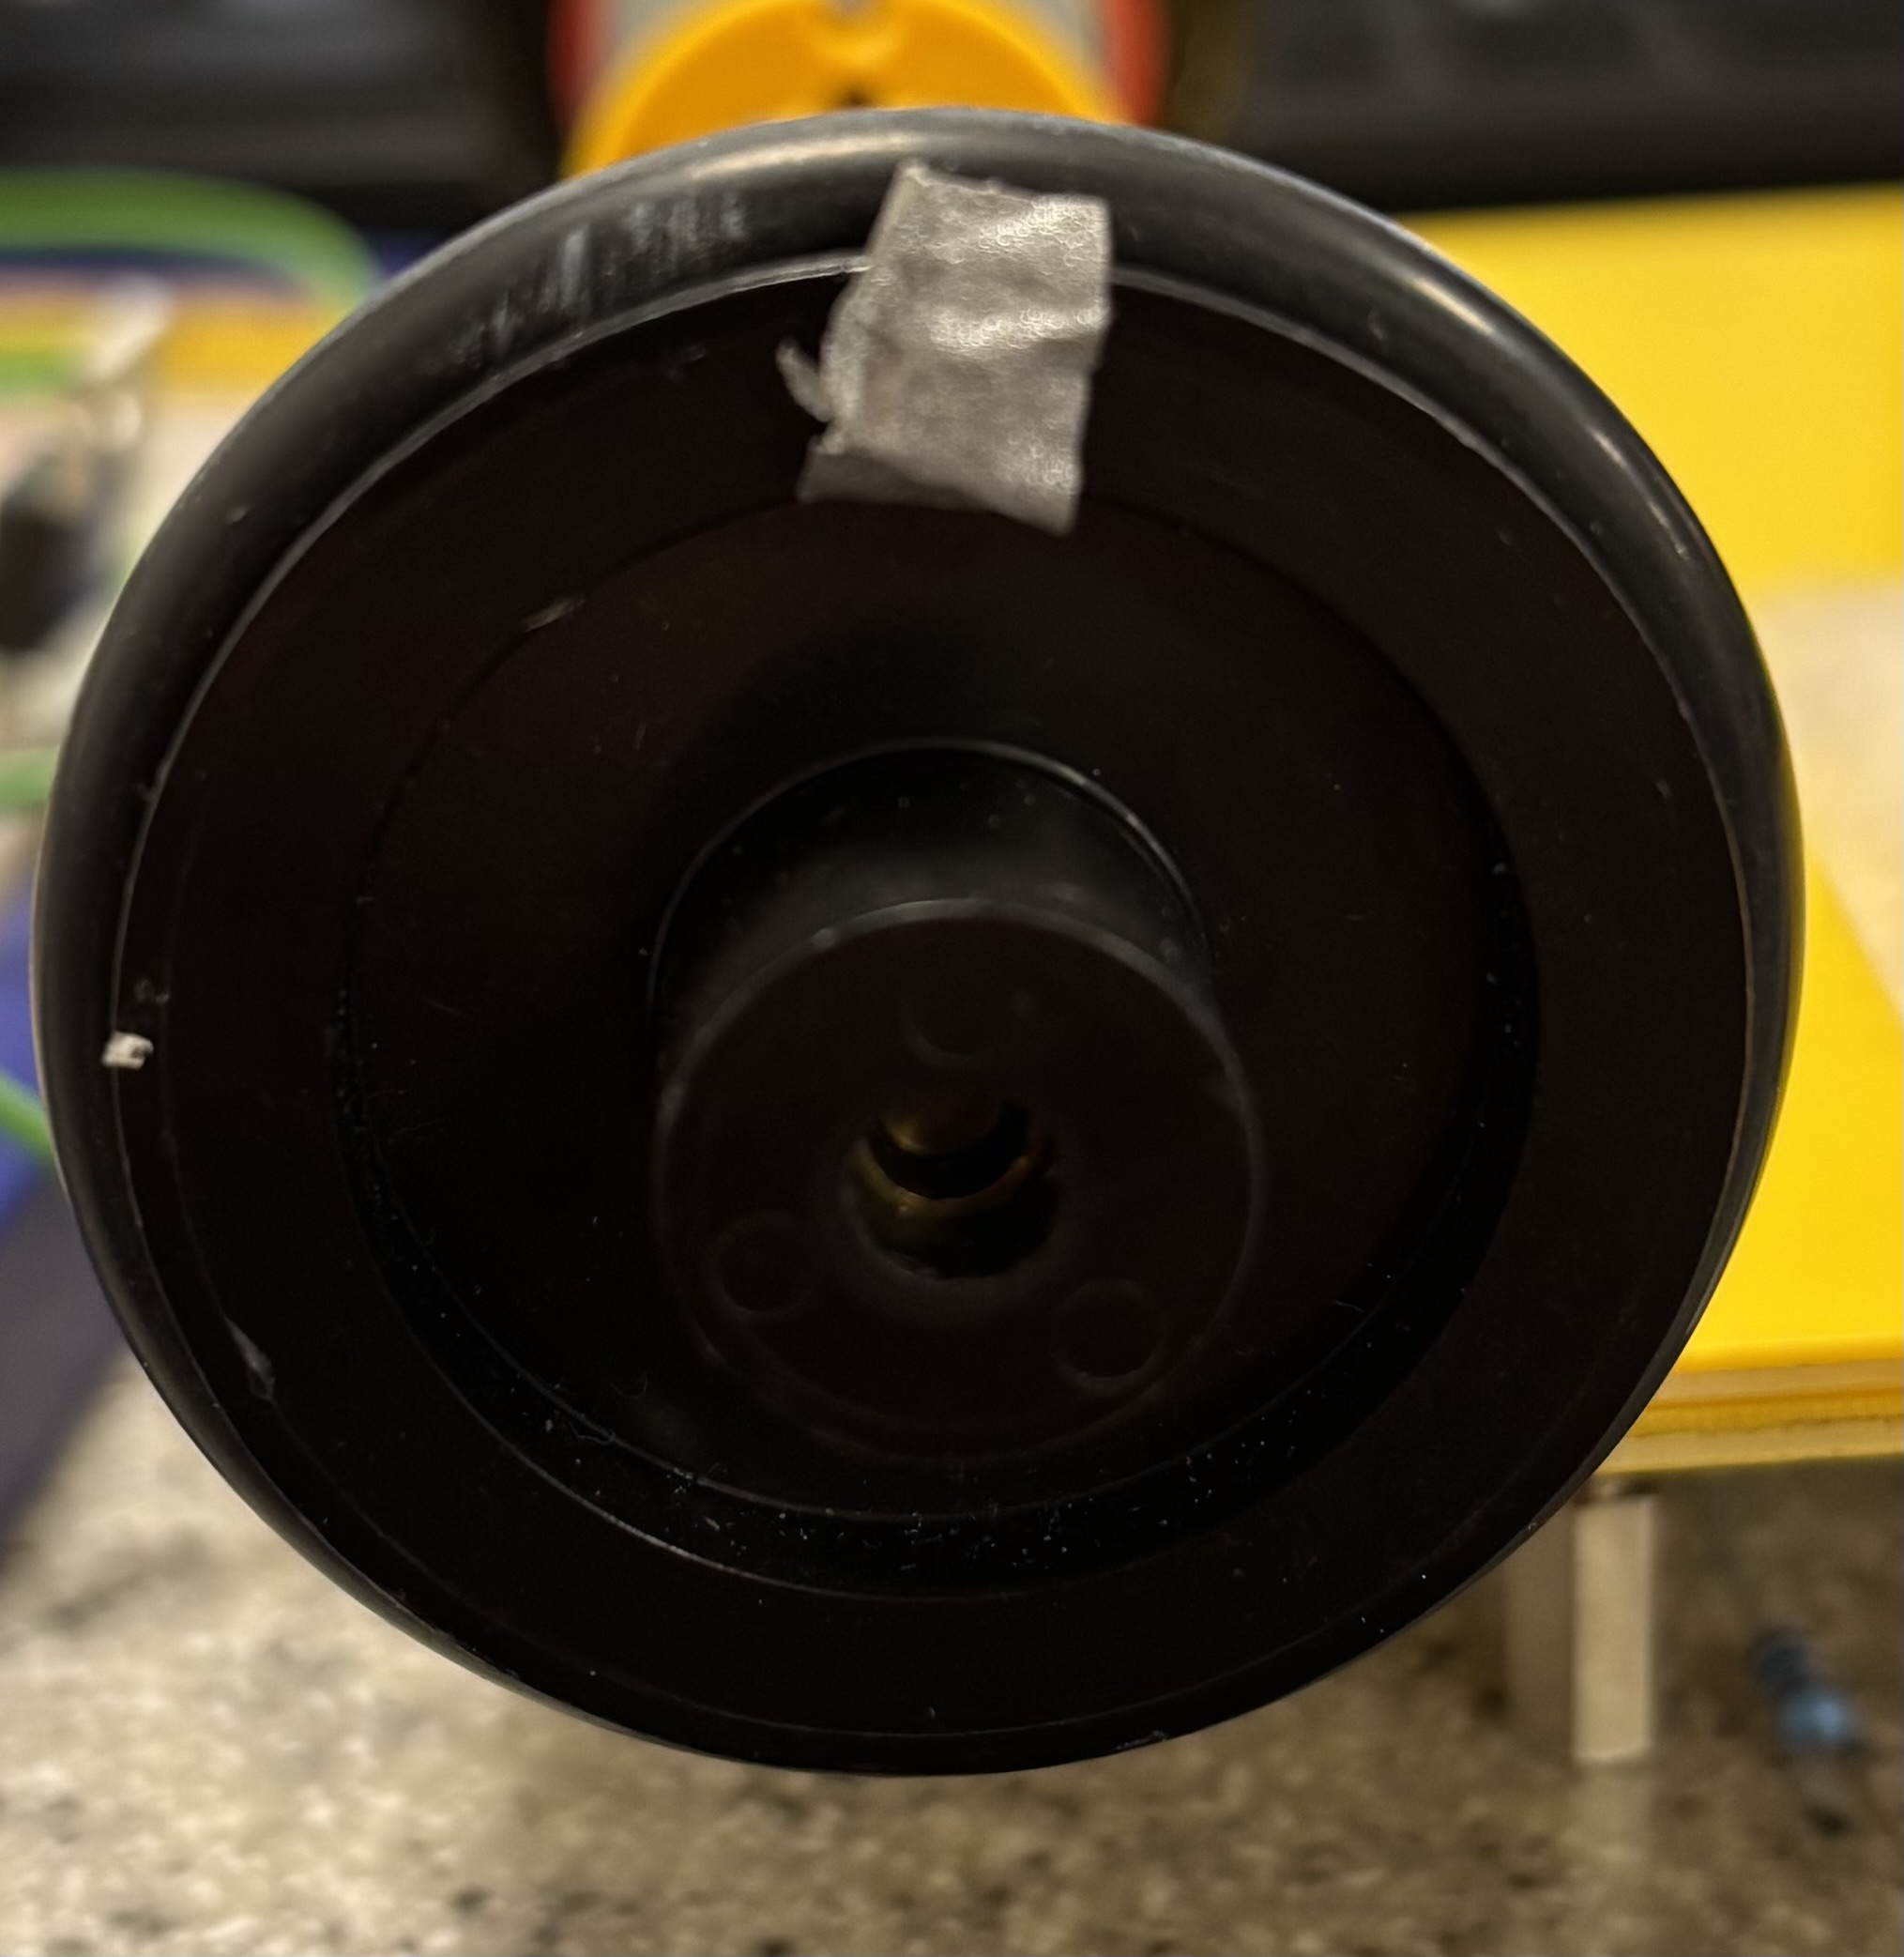
\includegraphics[height=0.8\linewidth]{photos/wheel_1.jpg}
        \caption{}
    \end{subfigure}
    \caption[Photographs of `mouse' wheel]{Photographs of `mouse' wheel: (a) `mouse' wheel with attached magnet (b) `mouse' wheel with tachometer tape over attached magnet}
    \label{fig:wheel_mag}
\end{figure*}

\subsection{Design D: Hall-Effect Sensor}
\label{sec:hes}
\label{sec:4}
Design D was built on a standard RH-32 breadboard reflecting the schematic shown in Fig.\ref{fig:hes_sensor_c}. First, the A3213EUA-T hall-effect sensor \cite{MicroSystems_2016} was placed at the edge of the breadboard. Since A3213EUA-T is an open-drain digital sensor, a \(10\) k\(\Omega\) pull-up resistor is connected from pin 1 (VDD) to pin 3 (VOUT). Second, the Arduino Nano Every was placed into the breadboard over the central channel, the GND, \(+5\) V Arduino supply and digital pin (D2) were connected to the hall-effect sensor as shown in Fig.\ref{fig:hes_sensor_c}. All circuit connections were kept short to maintain signal integrity and reduce the chance of EMI and noise.

\begin{figure}[H]
\centering
    \centering
    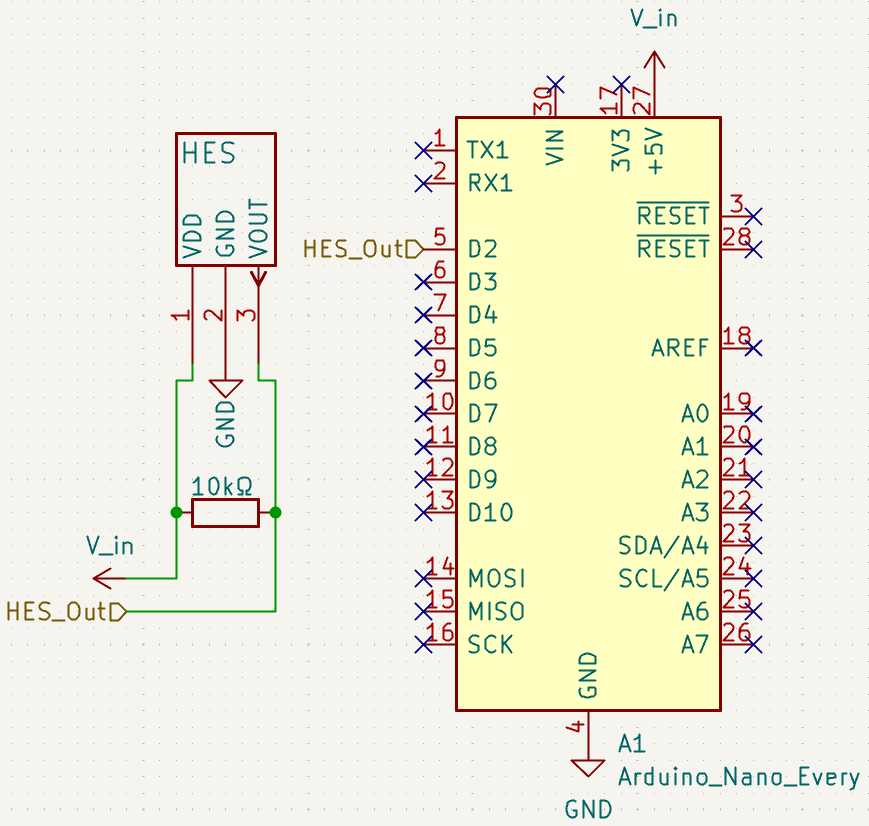
\includegraphics[width=0.7\linewidth]{circuits/hes_sensor.png}
    \caption[Design D: Schematic]{Schematic diagram of Design D; a Hall-effect sensor with \(10\) k\(\Omega\) pull-up resistor}
    \label{fig:hes_sensor_c}
\end{figure}

Finally, an Arduino program was developed and uploaded to the Arduino Nano Every  (Appendix \ref{app:Arduino} Listing \ref{cod:RPM}). The program utilised an interrupt service routine (ISR) to increment a global counter when a pulse was detected; the condition used was `FALLING'. The system recorded the time taken for four consecutive pulses, corresponding to four complete revolutions of the wheel, and subsequently calculated the rotational speed in RPM. The RPM value is then output to the serial interface. This approach allowed for the capturing of precise timestamps on interrupt-triggered events, minimising timing errors associated with polling, and by averaging the RPM calculation over four complete revolutions, the calculated output was a steadier more reliable RPM value.

\newpage
\subsubsection{Testing}
The steps for Testing Design D are as follows:

\begin{enumerate}
    \item The motor terminals \cite{mfa_motor} for the modified `mouse' wheel were connected to the \(6\) V DC range terminals of a KeySight E3631A variable power supply.
    \item The mouse chassis was then placed with the wheel facing the breadboard, magnet and tachometer tape towards the hall-effect sensor. The chassis was then moved till the distance between the sensor and wheel was \(\approx 1\) mm.
    \item The power supply was then turned on and set to a value of \(2\) V, and it was then noted if the hall-effect sensor was behaving as expected and tripping the interrupt correctly. The distance was then increased until the sensor stopped working; this distance was measured with a set of digital vernier callipers. Repeated three times to find an average.
    \item The distance between the sensor and the wheel was reduced back to \(\approx3\) mm (Photo of setup), the motor voltage was then set to \(1.0\) V. The RPM was measured thrice with an AT-6 tachometer, and three concurrent RPM calculated values from the Arduino Serial Monitor. The RPM values were recorded in Excel for later analysis. The voltage was then increased in increments of \(1.0\) V and measurements retaken till the motor voltage reached \(6.0\) V.
    \item The Keysight DSO1014A oscilloscope was connected to Design D, making sure the oscilloscope probe ratio matched the input signal ratio and the probe point was as close as possible to the hall-effect sensor. Channel 1 was connected to the sensor output `VOUT', and the probe reference was connected to GND.
    \item The distance between the sensor and the wheel was set back at \(\approx3\) mm, and motor voltage was set to \(3.0\) V. The steady-state waveform was observed and stored on an external USB as a CSV for later analysis in Excel.
\end{enumerate}

All measurements were taken after a 5-second stabilisation period to minimise transient effects and were conducted at room temperature (approximately 22°C). The oscilloscope output was imported into Excel and used to generate graphs for analysing rise and fall time. The tachometer and Arduino RPM readings were tabulated and averaged, statistical analysis was conducted to review the absolute error.

\subsection{Design E: Optical Feedback}
\label{sec:5}
\begin{figure}[H]
    \centering
    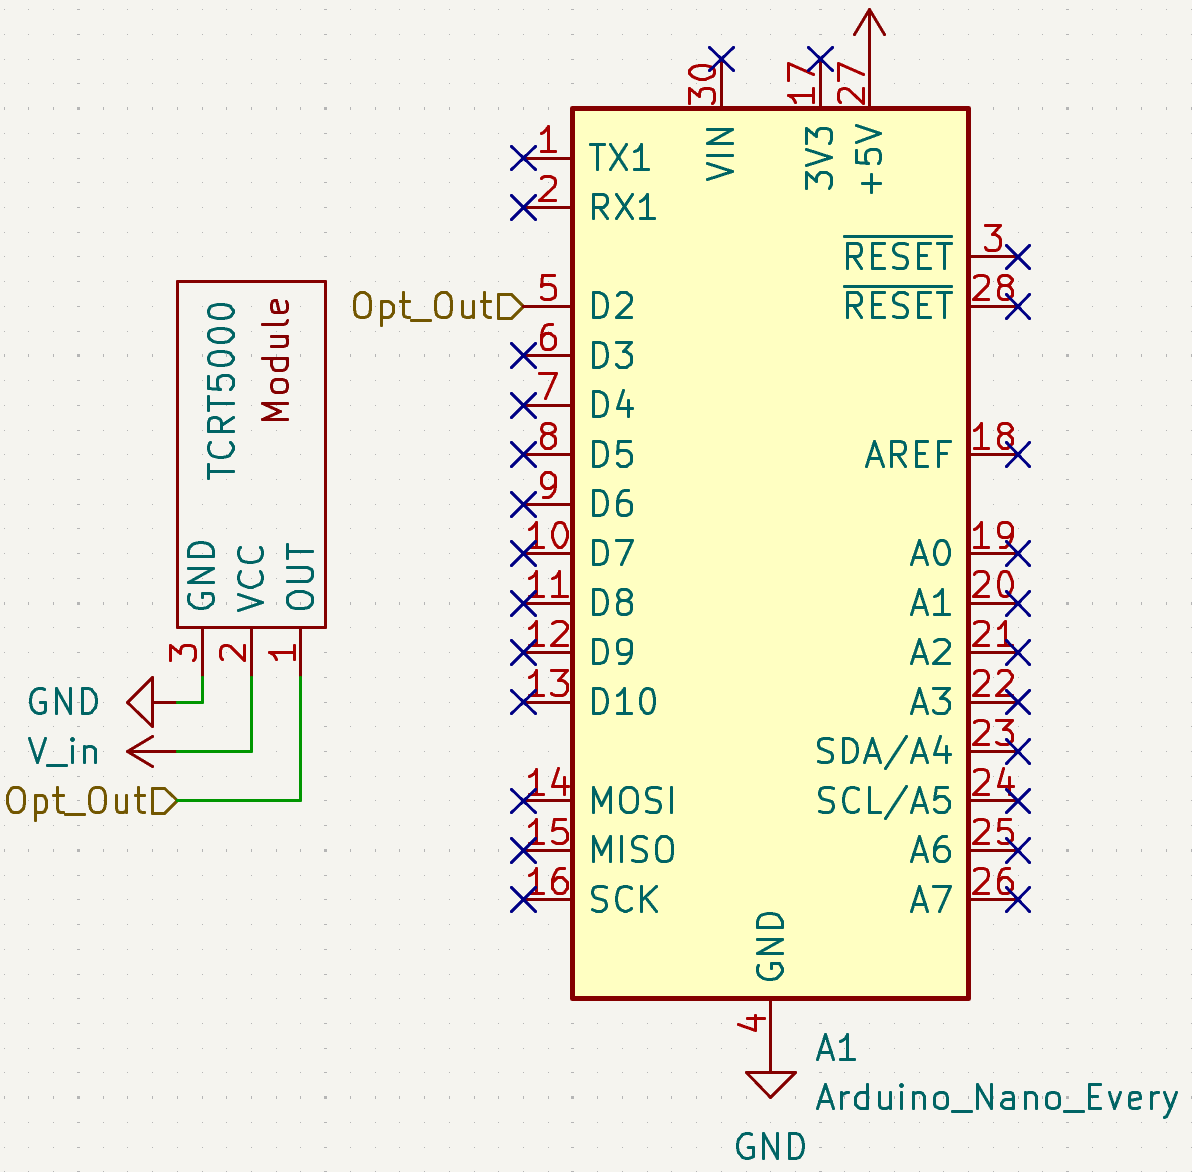
\includegraphics[width=0.75\textwidth]{circuits/opt_sensor.png}
    \caption[Design E: Schematic]{Schematic diagram of Design E; a Optical sensor module direct connections to Arduino Nano Every.}
    \label{fig:opt_sensor_c}
\end{figure}

Design E utilised a TCRT5000 optical sensing module \cite{Switch_TCRT5000}, made by Switch Electronics. Using breadboard jumper cables, the module was directly connected to the Arduino Nano Every as per the schematic Fig.\ref {fig:opt_sensor_c}. The RPM code (Appendix \ref{app:Arduino} Listing \ref{cod:RPM}) was re-uploaded to the Arduino Nano Every with the ISR updated to look for the `RISING' condition.

\subsubsection{Testing}
The testing method for Design D followed the same procedure as outlined in Section \ref{sec:hes}, except for the sensor being placed \(\approx5\) mm away during testing when distances are stated. All measurements were taken under the same conditions and analysed accordingly.


\newpage
\section{Results}
\subsection{Design D: Hall-Effect Sensor}
The average maximum distance observed before failure was \(\approx3\) mm (Appendix \ref{app:data} Table \hyperref[tab:A.5]{A.5}).

As summarised in Table \ref{tab:HES_VoltRPM} the hall-effect sensor Arduino RPM values are consistent with the tachometer reference values, with deviation remaining within \(\pm 0.54\%\). This variation in values is due to the integer nature of the Arduino RPM calculation, reducing potential accuracy.

\begin{table}[H]
    \centering
    \caption[Design D: RPM Measurements]{Hall-effect sensor Arduino Calculated RPM compared to measured Tachometer RPM at varying voltages from \(1.0\rightarrow6.0\) V (Appendix \ref{app:data} Table \hyperref[tab:A.4]{A.4}). The tachometer took readings at an accuracy of 4 s.f. and the Arduino calculated RPM values were set to be integers.}
    \label{tab:HES_VoltRPM}
    \begin{tabular}{|c||c|c|c|c|}\hline
    &\multicolumn{2}{|c|}{RPM} &  &\\\hline
    Voltage (V)&Tachometer Average&Arduino Average&Absolute Error &Percentage Error\\ \hline 
    1.0&131.3&132 &-0.7&0.54\\ \hline
    2.0&350.3&350 &0.3&0.10\\\hline
    3.0&566.0&566 &0.0&0.00\\\hline
    4.0&759.3&759 &0.2&0.03\\\hline
    5.0&982.9&983 &-0.1&0.01\\\hline
    6.0&1176&1175 &0.0&0.00\\\hline\end{tabular}  
\end{table}

Observing and analysing the output waveforms from the A3213EUA-T on the DSO1014A oscilloscope (Fig.\ref{fig:hes_osc}) when triggered, the fall time of the signal to a steady state is \(\approx0.04\) \(\mu\)s and the signal has a rise time of \(\approx2.25\) \(\mu\)s to steady state. The signal has a clean edge with no oscillation, indicating a strong digital signal.

\begin{figure*}[h!]
    \centering
    \begin{subfigure}{0.8\textwidth}
        \centering
        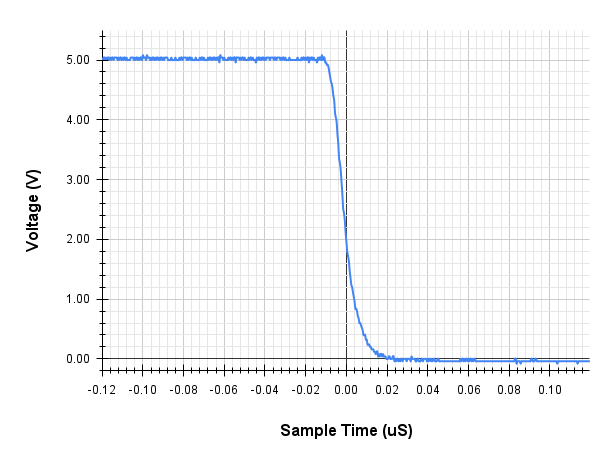
\includegraphics[width=1\linewidth]{graphs/hes_f_osciliscope.png}
        \caption{}
    \end{subfigure}
    \begin{subfigure}{0.8\textwidth}
        \centering
        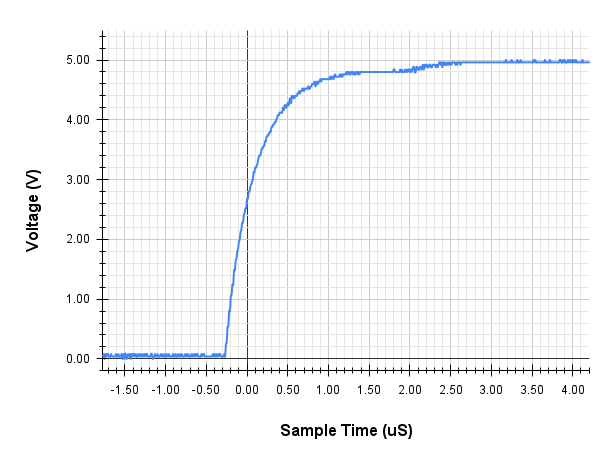
\includegraphics[width=1\linewidth]{graphs/hes_r_osciliscope.png}
        \caption{}
    \end{subfigure}
    \caption[Design D: Oscilliscope Rise and Fall]{A3213EUA-T output waveform from a DSO1014A oscilloscope, split into rise and fall conditions: (a) Falling signal edge (b) Rising signal edge}
    \label{fig:hes_osc}
\end{figure*}

\subsubsection{Cost of Implementation}

\begin{table}[H]
\centering
\caption{Alphabetically Ordered Estimated Component Costs for Design D}
\label{tab:design_d_cost}
\begin{tabularx}{\linewidth}{|l|X|X|X|}
\hline
\textbf{Component} & \textbf{Quantity} & \textbf{Unit Price (£)} & \textbf{Total Price (£)}\\ \hline
10kΩ Through-Hole Resistor \cite{rs_10kresistor}& 1 & 0.07 & 0.07\\ \hline
Allegro A1101EUA-T Hall-Effect Sensor IC \cite{MicroSystems_2016}& 1 & 0.69 & 0.69\\ \hline
Neodymium Magnet 10mm x 3mm \cite{RS_2192257} & 1 & 0.11 & 0.11\\ \hline\hline
\textbf{Total Estimated Cost} & & & \textbf{£0.87}\\ \hline
\end{tabularx}
\end{table}

Table \ref{tab:design_d_cost} details the individual components required to implement Design E, alongside their quantities, suppliers and unit costs based on UK-sourced pricing at the time of writing.

\newpage
\subsection{Design E: Optical Feedback}
The average maximum distance observed before failure was \(\approx13\) mm (Appendix \ref{app:data} Table \hyperref[tab:A.7]{A.7}).

As summarised in Table \ref{tab:Opt_VoltRPM} the optical sensor Arduino RPM values are consistent with the tachometer reference values, with deviation remaining within \(\pm 0.75\%\). This variation in values is due to the integer nature of the Arduino RPM calculation, reducing potential accuracy.

\begin{table}[H]
    \centering
\caption[Design E: RPM Measurements]{Optical sensor Arduino calculated RPM compared to measured Tachometer RPM at varying voltages from \(1.0\rightarrow6.0\) mm (Appendix \ref{app:data} Table \hyperref[tab:A.6]{A.6}). The tachometer took readings at an accuracy of 4 s.f. and the Arduino calculated RPM values were set to be integers.}
\label{tab:Opt_VoltRPM}
    \begin{tabular}{|c||c|c|c|c|}\hline
    &\multicolumn{2}{|c|}{RPM} &  &\\\hline
    Voltage (V)&Tachometer Average&Arduino Average&Absolute Error &Percentage Error\\ \hline 
    1.0&128.6&129&-0.4&0.29\\ \hline
    2.0&352.6&350&2.6&0.75\\\hline
    3.0&565.1&567&-1.9&0.34\\\hline
    4.0&760.2&760&0.2&0.03\\\hline
    5.0&982.9&983&-0.1&0.01\\\hline
    6.0&1174&1174&0.0&0.00\\\hline\end{tabular}  
\end{table}

Observing and analysing the output waveforms from the TCRT5000 sensor module on the DSO1014A oscilloscope (Fig.\ref{fig:opt_osc}) when triggered, the fall time of the signal is \(\approx0.045\) \(\mu\)s and the signal has a rise time of \(\approx0.045\) \(\mu\)s. The signal has oscillations when changing state, indicating a weaker digital signal.

\begin{figure*}[h!]
    \centering
    \begin{subfigure}{0.8\textwidth}
        \centering
        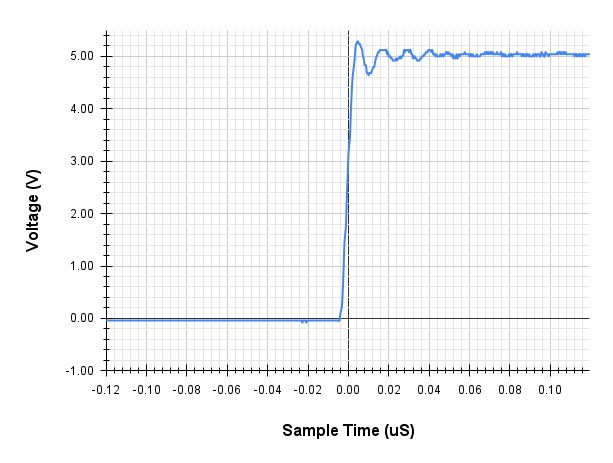
\includegraphics[width=1\linewidth]{graphs/opt_r_osciliscope.png}
        \caption{}
    \end{subfigure}
    \begin{subfigure}{0.8\textwidth}
        \centering
        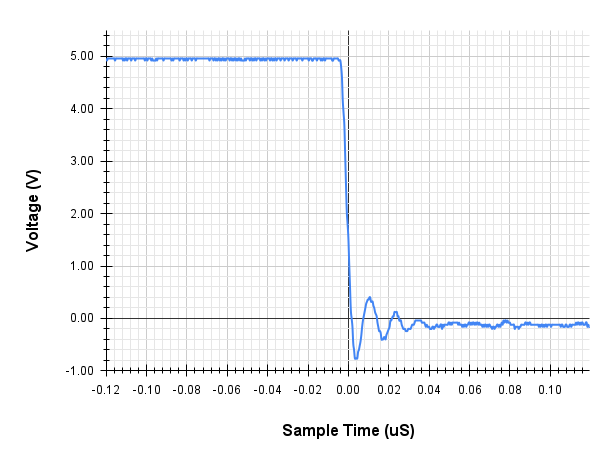
\includegraphics[width=1\linewidth]{graphs/opt_f_osciliscope.png}
        \caption{}
    \end{subfigure}
    \caption[Design E: Oscilliscope Rise and Fall]{Hall-effect sensor output waveform from a DSO1014A oscilloscope, split into rise and fall conditions: (a) Rising signal edge (b) Falling signal edge}
    \label{fig:opt_osc}
\end{figure*}

\subsubsection{Cost of Implementation}
\begin{table}[H]
\centering
\caption{Alphabetically Ordered Estimated Component Costs for Design E}
\label{tab:design_e_cost}
\begin{tabularx}{\linewidth}{|l|X|X|X|}
\hline
\textbf{Component}                                   & \textbf{Quantity} & \textbf{Unit Price (£)} & \textbf{Total Price (£)} \\ \hline
Infrared Line Tracking Sensor Module (TCRT5000) \cite{Switch_TCRT5000} & 1 & 1.37  & 1.37\\ \hline
RS Reflective Tachometer Tape \cite{RS_8459731}& 1 & 0.87 & 0.87\\ \hline\hline
\textbf{Total Estimated Cost}                        &   &       & \textbf{£2.24} \\ \hline
\end{tabularx}
\end{table}

Table \ref{tab:design_e_cost} details the individual components required to implement Design E, alongside their quantities, suppliers and unit costs based on UK-sourced pricing at the time of writing.

\newpage
\section{Discussion}
This section evaluates two design solutions proposed to facilitate the addition of a speed feedback system to improve the control loop currently implemented in the `mouse' design. Both designs worked as expected and provide a reliable RPM value. Design D (HES) may be a more appropriate solution as it provides a potential learning opportunity in magnetic sensing and related components, and not a plug-and-play module. 

\subsubsection{Design Performance}
Design D provided a consistent and reliable RPM. However, the HES and trigger magnet must be within 3mm (Appendix \ref{app:equip&test} Figure \ref{fig:hes_distance_measurements}) of each other to provide accurate detection.

Design E provided a stable and accurate RPM. To avoid false positives, the distance between the sensor and reflective tape should be no more than 5mm (Appendix \ref{app:equip&test} Figure \ref{fig:opt_distance_measurements}). In addition, it is recommended that the wheel's surface be non-reflective.

\subsubsection{Complexity}
Both Design D and E would be easy to introduce into the `mouse' platform, with various levels of documentation to assist in assembly. However, it is easier to position the HES sensor than the optical module. On the other hand, Design D requires chassis modification in the addition of a magnet to the wheel.

\subsubsection{Cost}
When comparing the cost of implementation, Design D is the preferable option, only introducing a cost estimate per `mouse' of £0.87, which is £1.37 less than the cost of Design E's implementation, which is £2.24. However, these costs do not account for the potential technician time to modify the `mouse' chassis.

\subsubsection{Further Investigations}
Additional research should be conducted on incorporating the RPM measurement into a working ‘mouse’ control loop. In addition, a potential investigation could be conducted on creating an IR optical sensor circuit instead of a pre-fabricated module.

\subsubsection{Recommendations}
Both Design D and E could be used to great effect on the `mouse' platform. However, I suggest Design D as the most appropriate option, as it provides learning opportunities and reliable, cost-effective RPM measurements.

\chapter{Current Feedback}
\section{Overview}
\label{sec:overview_motor}
The key focus of this section is the discussion of adding a current feedback sub-system to the autonomous `mouse', addressing the limitation that does not allow for motor current sensing, meaning deteriorating battery health and current spikes during hill ascent cannot be considered when controlling motor speed. The section suggests altering the motor drive sub-system of the `mouse' to add motor current feedback. The motor drive sub-system currently varies the voltage across a \(6\) V DC motor \cite{mfa_motor} using a MOSFET or BJT acting as an electronic switch, toggling on and off with a PWM control signal \cite{Robinson2025}. The proposed solutions must provide reliable, accurate current readings and not adversely affect motor drive control. The solutions will be evaluated based on their stability, simplicity of integration and cost of implementation.

\section{Design Concepts and Methods}
\subsubsection{Shunt Resistor}
\begin{wrapfigure}{r}{0.4\textwidth}
  \begin{center}
    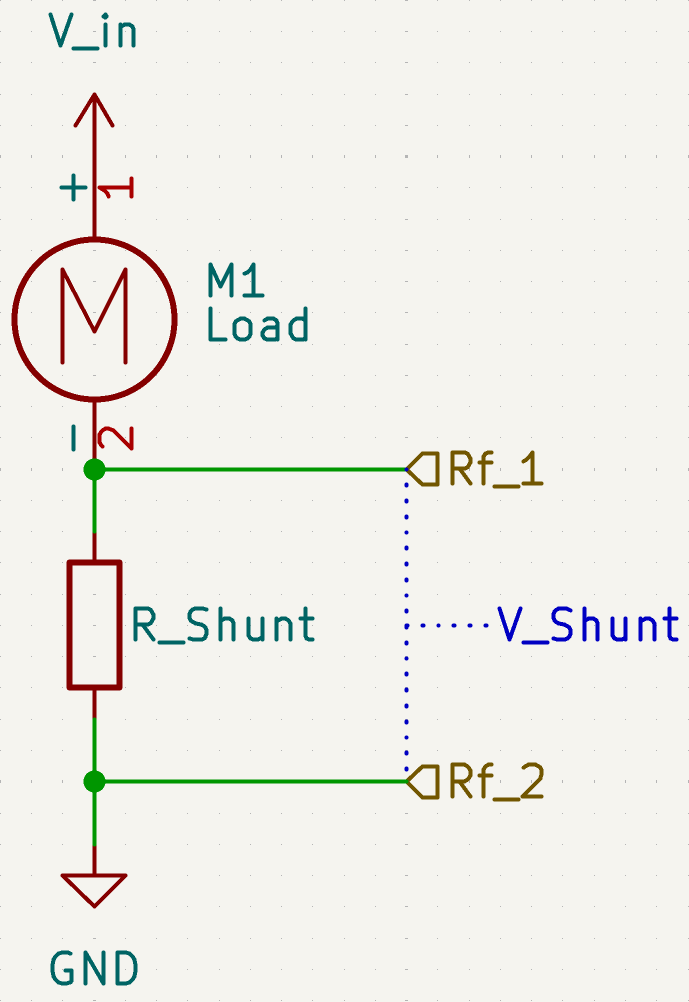
\includegraphics[width=1\linewidth]{circuits/shun_res_theory.png}
  \end{center}
  \caption{Shunt Resistor Circuit with a motor as circuit load.}
  \label{fig:shunt_theory}
\end{wrapfigure}

Designs F and G utilise a shunt resistor to measure the current within the motor. Generally, a shunt resistor is a precision low-resistance device connected in series with the load (Fig.\ref{fig:shunt_theory}), ensuring that the load current flows through it and generating a voltage directly related to the magnitude of the current as per Ohm's Law:

\begin{equation}
    V=IR
    \label{equ:Ohms_law}
\end{equation}

The potential difference (voltage drop) is measured across the terminals of the shunt resistor. Rearanging equation \ref{equ:Ohms_law} for \(I\) in terms of \(V\) and \(R\) (Equation \ref{equ:Ohms_law_current}), you can calculate the current from the known resistance and measured voltage.
\begin{equation}
    I=\frac{V}{R}
    \label{equ:Ohms_law_current}
\end{equation}

Shunt resistor values are commonly in the milliohm range to suit different current sensing applications. By choosing a smaller resistance the voltage drop across the shunt resistor will be smaller, and reducing the voltage drop into the millivolt range can minimise power loss and circuit disruption.  The small voltage developed is commonly amplified to improve signal accuracy before further processing.


\subsection{Design F: Low-Side Motor Drive}
\label{sec:low_motor}
\begin{wrapfigure}{r}{0.5\textwidth}
  \begin{center}
    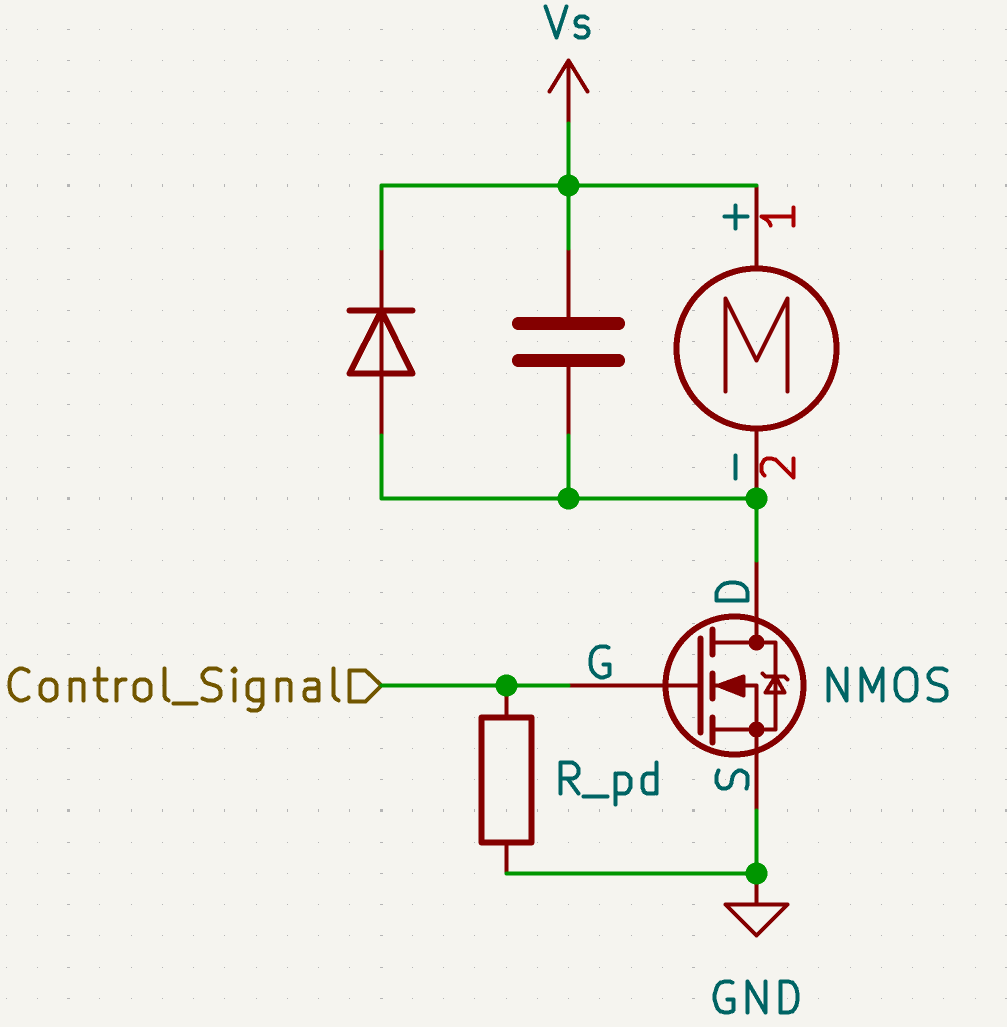
\includegraphics[width=1\linewidth]{circuits/low_side_mos.png}
  \end{center}
  \caption[Low-side N-channel MOSFET Motor Drive Circuit]{Low-side N-Channel MOSFET drive circuit controlling a DC Motor Load with transient suppression components.}
  \label{fig:low_drive_theory}
\end{wrapfigure}

Design F used a low-side N-channel MOSFET drive circuit (Fig.\ref{fig:low_drive_theory}) to control the operation of a DC motor. The MOSFET acts as an electronic switch in this configuration, enabling or disabling current flow through the motor. When acting like a switch the N-channel MOSFET must have a gate-source voltage (\(V_{GS}\)), defined as \(V_{GS}=V_G-V_S\), sufficiently above the threshold voltage (\(V_{t}\)) potential for reliable conduction \cite[p.297]{Sedra_Smith_Microelectronic}. The gate voltage (\(V_{G}\)) is supplied by a control signal applied to the gate terminal (`Control\_Signal'), and the source voltage (\(V_s\)) is set to GND.

Varying the duty cycle of the control signal modulates the average voltage and current supplied to the motor, providing adjustable speed control. When the signal is high the MOSFET conducts and the inverse is true when the circuit is low. The voltage observed can be calculated using equation \ref{equ:pwm_volt} as described by Rashid \cite[p. 920]{Muhammad_PowerElectronics}; where \(v\) is the voltage observed, \(V_{s}\) is the supply voltage and \(\delta\) is the normalised duty cycle (\(0\rightarrow1.0\)).

\begin{equation}
    v = \delta V_{s}
    \label{equ:pwm_volt}
\end{equation}
\vspace{1em}

Furthermore, a pull-down resistor (`R\_pd') is utilised within the circuit connecting the gate and source of the transistor; this prevents the gate voltage from floating and pulls it to the same potential (GND) when the signal is low, closing the MOSFET switch.

In addition, as DC motors are inductive loads, switching them introduces transient voltage spikes. The voltage spikes are particularly obvious during turn-off events. To address the voltage spikes and increase stability it is common practice to add:

\begin{itemize}
    \item A flyback diode is placed directly across the motor terminals \cite[pp.970-971]{Muhammad_PowerElectronics}, with its cathode connected to the top of the motor. This provides a path for the inductive current from the motor when the MOSFET switches off, safely clamping the voltage spike and protecting the MOSFET from overvoltage conditions.
    \item A snubber capacitor is placed across the motor terminals \cite[p.380]{Williams_EMC} to suppress high-frequency voltage transients and reduce EMI generated by the DC motor.
\end{itemize}


\subsection{Design G: High-Side Motor Drive}
\label{sec:highside}
\begin{figure}[H]
    \centering
    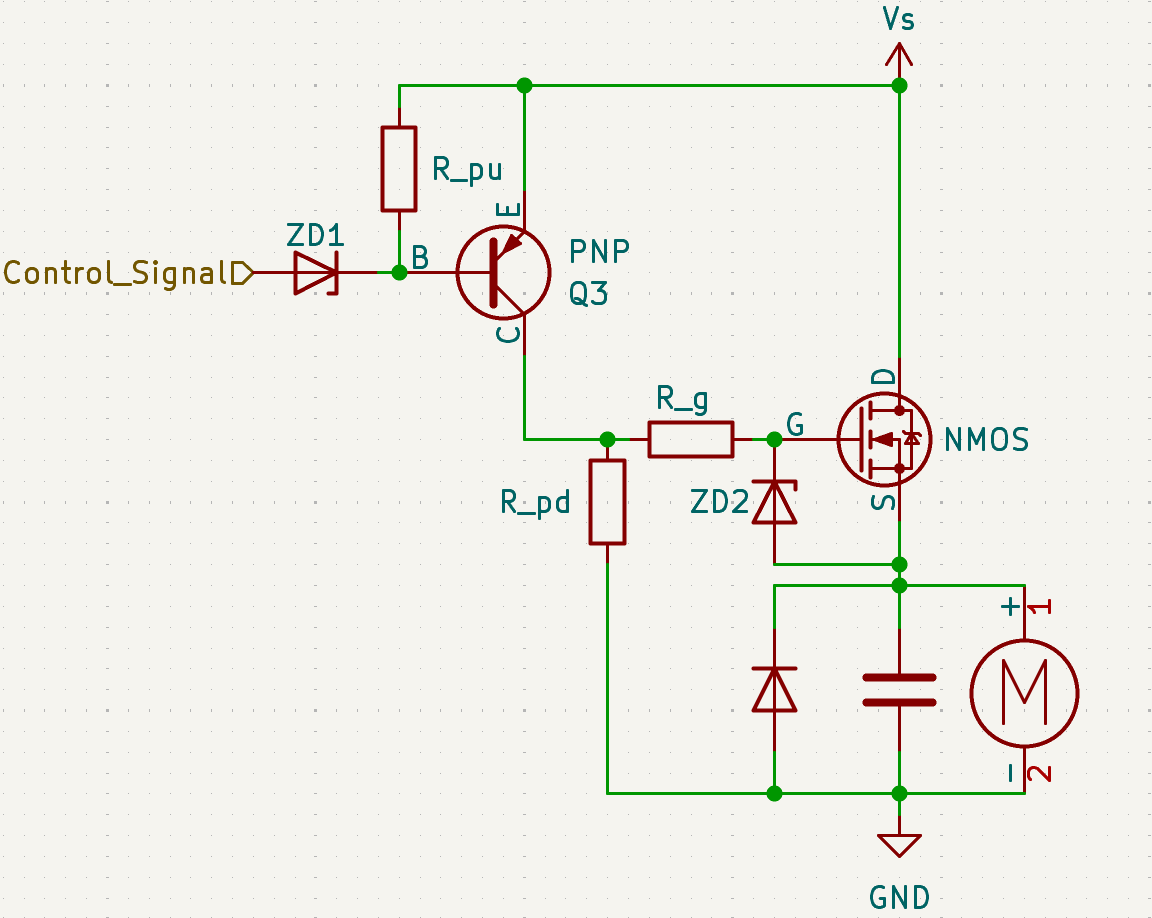
\includegraphics[width=1\linewidth]{circuits/high_side_mos.png}
    \caption[High-side N-channel MOSFET Motor Drive Circuit]{Schematic of a High-side N-channel MOSFET motor drive circuit with PNP transistor level-shifting stage. Controlling a DC motor with transient suppression components.}
    \label{fig:high_drive_theory}
\end{figure}

Design G used a high-side N-channel MOSFET drive circuit (Fig.\ref{fig:high_drive_theory}) to control the operation of a DC motor. Using a high-side switch allows the load to be directly connected to GND. However, driving an N-channel MOSFET in a high-side position presents a challenge, as the gate-source voltage (\(V_{GS}\)) must be raised sufficiently to turn the device on and in a high-side position when conducting the source is connected to the voltage supply (\(V_s\)).

A PNP transistor level-shifting stage is employed to overcome this, shifting the input control signal to the \(V_s\) level, enabling a low-voltage logic-level control signal to switch the high-side N-channel MOSFET. A PNP transistor works by allowing a current to flow from the emitter to the collector when there is sufficient current observed from the emitter to base (forward-bias) \cite[p.246]{Sedra_Smith_Microelectronic}.

The control signal (`Control\_Signal') is applied to the PNP base via a series-connected zener diode (`ZD2'). Adding a zener diode provides overvoltage protection, ensuring that the PNP transistor’s base-emitter junction remains within its safe operating limits. A pull-up resistor (`R\_pu') is connected between the PNP transistor’s base and the positive supply rail, keeping the transistor turned off when the control signal is floating or at a logic-high level. When the signal transitions low, the base-emitter junction of the PNP transistor becomes forward-biased, turning the transistor on. This action connects the emitter to the collector, allowing the positive supply rail to connect to the N-Channel MOSFET’s gate terminal via a gate resistor (`R\_g'). As previously discussed in Section \ref{sec:low_motor}, as the gate voltage rises it exceeds the MOSFET’s source potential (at the same potential as the supply rail \(`V_s\) during conduction), allowing current to flow from the drain to the source pin and hence through the motor load to GND.

The gate resistor performs two key tasks within this circuit, primarily limiting the current into the gate terminal, which controls the transistor's switching speed. Additionally, the resistor protects the PNP transistor from transient currents observed during transistor switching events. Typically, gate resistor values are between \(1\rightarrow100\Omega\) when used in a motor drive circuit. To further improve system robustness, a zener diode (`ZD2') is placed across the MOSFET’s gate and source terminals. The zener clamps the gate voltage (\(V_G\)) to a safe maximum value, protecting the MOSFET from overvoltage conditions.

The motor load circuit and pull-down resistor (`R\_pd') are included as per the details outlined in Section \ref{sec:low_motor}, the main difference being that the motor load now connects to the MOSFET source pin and GND.

It should be noted that with this design, the PWM response is inverted. When the PWM control signal is low the N-Channel MOSFET is conducting the inverse is true when the signal is high.

\section{Procedures}
\subsection{Design F: Low-Side Motor Drive}
\label{sec:low_side_motor}
\label{sec:6}
\subsubsection{Assembly}
\begin{figure}[H]
    \centering
    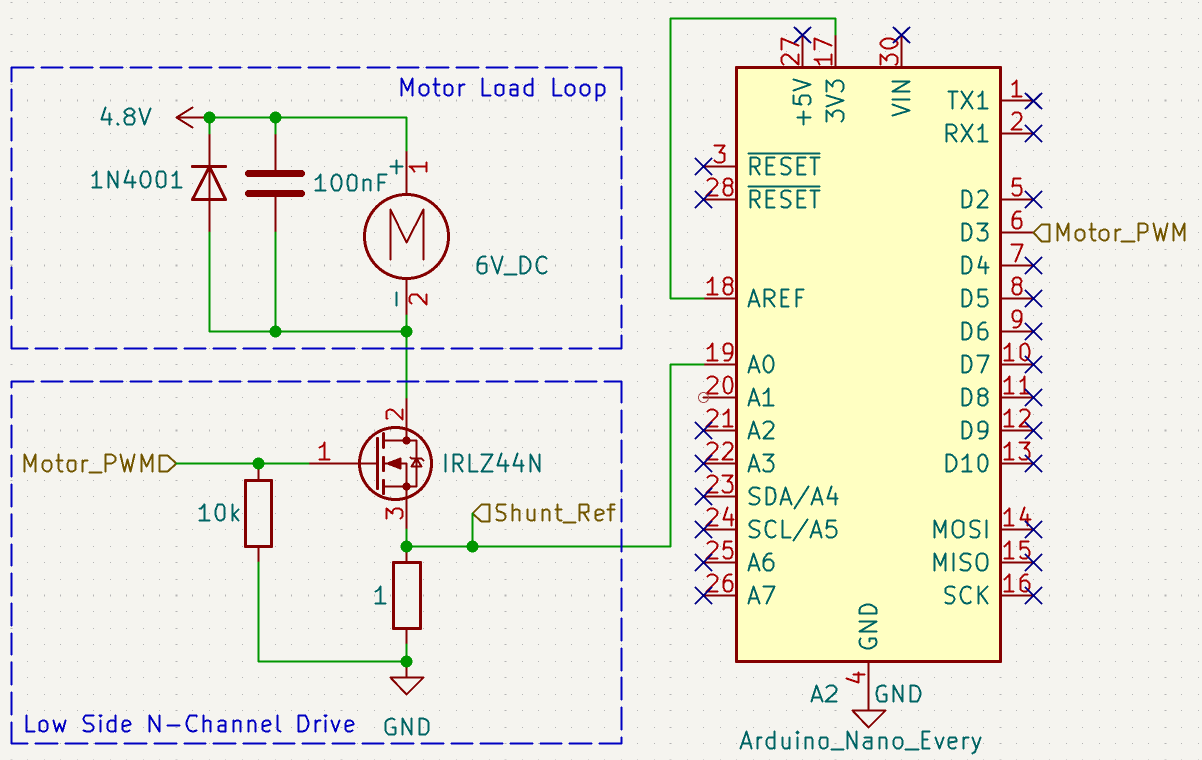
\includegraphics[width=1\linewidth]{circuits/current_low.png}
    \caption[Design F: Schematic]{Schematic diagram of Design F; a Low-side motor drive circuit with current sensing shunt resistor.}
    \label{fig:low_current_circuit}
\end{figure}

Design F was built on a standard RH-32 breadboard following the design outline in Figure \ref{fig:low_current_circuit}. Firstly, the N-Channel drive circuit was assembled using an IRLZ44N N-Channel MOSFET \cite{Infineon_IRLZ44N}; the source (pin 3) of the MOSFET was connected to the \(1\) \(\Omega\)  current sensing shunt resistor in series to GND and the gate (pin 1) is connected to the GND with a \(10\) k\(\Omega\) pull-down resistor. The IRLZ44N was choosen for its logic level of \(3.3\) V (Matches Arduino PWM \cite{Microchip_ATmega4809}) and previous use in the `mouse' race as a MOSFET switch.

Secondly, the motor load loop was assembled using a motor from a mouse chassis. First, the motor was connected to the breadboard with single-core wires. Following on, a 1N4001 \cite{Kitronik_1N4001} flyback diode and \(100\) nF snubbing capacitor were connected over the motor as seen in Figure \ref{fig:low_current_circuit}. Care was taken in orienting the 1N4001 making sure the anode was connected to the top of the motor. After that the \(4.8\) V DC 3631A lab power supply rail was connected to the top side of the motor.

Third, the Arduino Nano Every \cite{Arduino_Every} was placed into the breadboard over the central channel. The analogue pin was connected first with A0 connecting to the node between the MOSFET and resistor (Shunt\_Ref). The D3 pin (Motor\_PWM) was then connected to the gate of IRLZ44N. Following on, the GND was connected to the Arduino and the \(3.3\) V DC supply rail from the Arduino was connected to the analogue reference (AREF) pin of the Arduino. By setting the AREF at \(3.3\) V DC the ADC within the Arduino Nano could measure at increments of \(\approx3.2\) mV (LSB) with an accuracy of \(\pm0.5\)LSB \cite{Microchip_ATmega4809}. 

Finally, an Arduino program was developed and uploaded to the Arduino Nano Every (Appendix \ref{app:Arduino} Listing \ref{cod:current_1ref}). The program controlled the speed of the DC motor via Pulse Width Modulation (PWM) and monitored the current drawn by the motor. The PWM duty cycle was adjusted within the code to set the motor’s operating speed. The current was measured using one reference point (`Shunt\_Ref') achieved through the analogue input pin A0. The potential difference between the reference point and GND was recorded, and the value was then stored in an array. A moving average algorithm was implemented within the program and calculated based on the array values. The average calculated value was then converted into a current using equation \ref{equ:Ohms_law_current}, as the resistance was \(1\Omega\) the value was directly converted from voltage to current. This value was multiplied by a constant of \(0.0032\) (\(3.3V/1024\approx0.0032\))to convert from the digital signal to an analogue value. This approach allowed for a smoother, more representative current value for each operating condition. The processed current data was then output via the Arduino’s serial interface. 

\subsubsection{Testing}
The steps for Testing Design F are as follows:

\begin{enumerate}
    \item Design F power supply rails and circuit GND were verified using a KeySight 34450A multimeter.
    \item The `Motor\_PWM' was varied from \(0\rightarrow128\) incrementing in values of 8, representing a duty cycle range \(0\rightarrow50\%\). The motor voltage and current were measured thrice at each PWM value using a KeySight 34450A multimeter. The voltage values were recorded in Excel and compared to the expected voltages. In addition, the motor current values were recorded in Excel along with the Arduino calculated current values seen on the Serial Monitor.  
    \item More current readings were then taken from the motor and Arduino whilst applying slight resistance to the wheel, whilst the `Motor\_PWM' was varied from \(0\rightarrow128\) incrementing approximating to a 10\% change in duty cycle, recording values in Excel.
\end{enumerate}

During testing, it was noted that the voltage readings over the motor seemed to be off expectations (Appendix \ref{app:data} Table 5). Waveform's on the oscilloscope suggested the back EMF voltage from the motor seriously impacted readings (Appendix \ref{app:data} Figure \ref{fig:osc_emf}). A secondary test was completed, replacing the motor load loop with a \(1\) k\(\Omega\) resistor connected to the \(4.8\) V DC 3631A lab power supply rail and pin 2 (Drain) of IRLZ44N. The `Motor\_PWM' was varied \(0\rightarrow128\) incrementing in values approximating to a 10\% change in duty cycle. The voltage across its terminals was then measured using the KeySight 34450A multimeter, recording values in Excel. 

All measurements were taken after a 5-second stabilisation period to minimise transient effects and were conducted at room temperature (approximately 22°C). The multimeter readings were tabulated, and statistical analysis was performed to evaluate the motor's PWM response and the absolute error for the current readings.



\subsection{Design G: High-Side Motor Drive}
\label{sec:7}
\subsubsection{Assembly}

\begin{figure}[H]
\centering
    \centering
    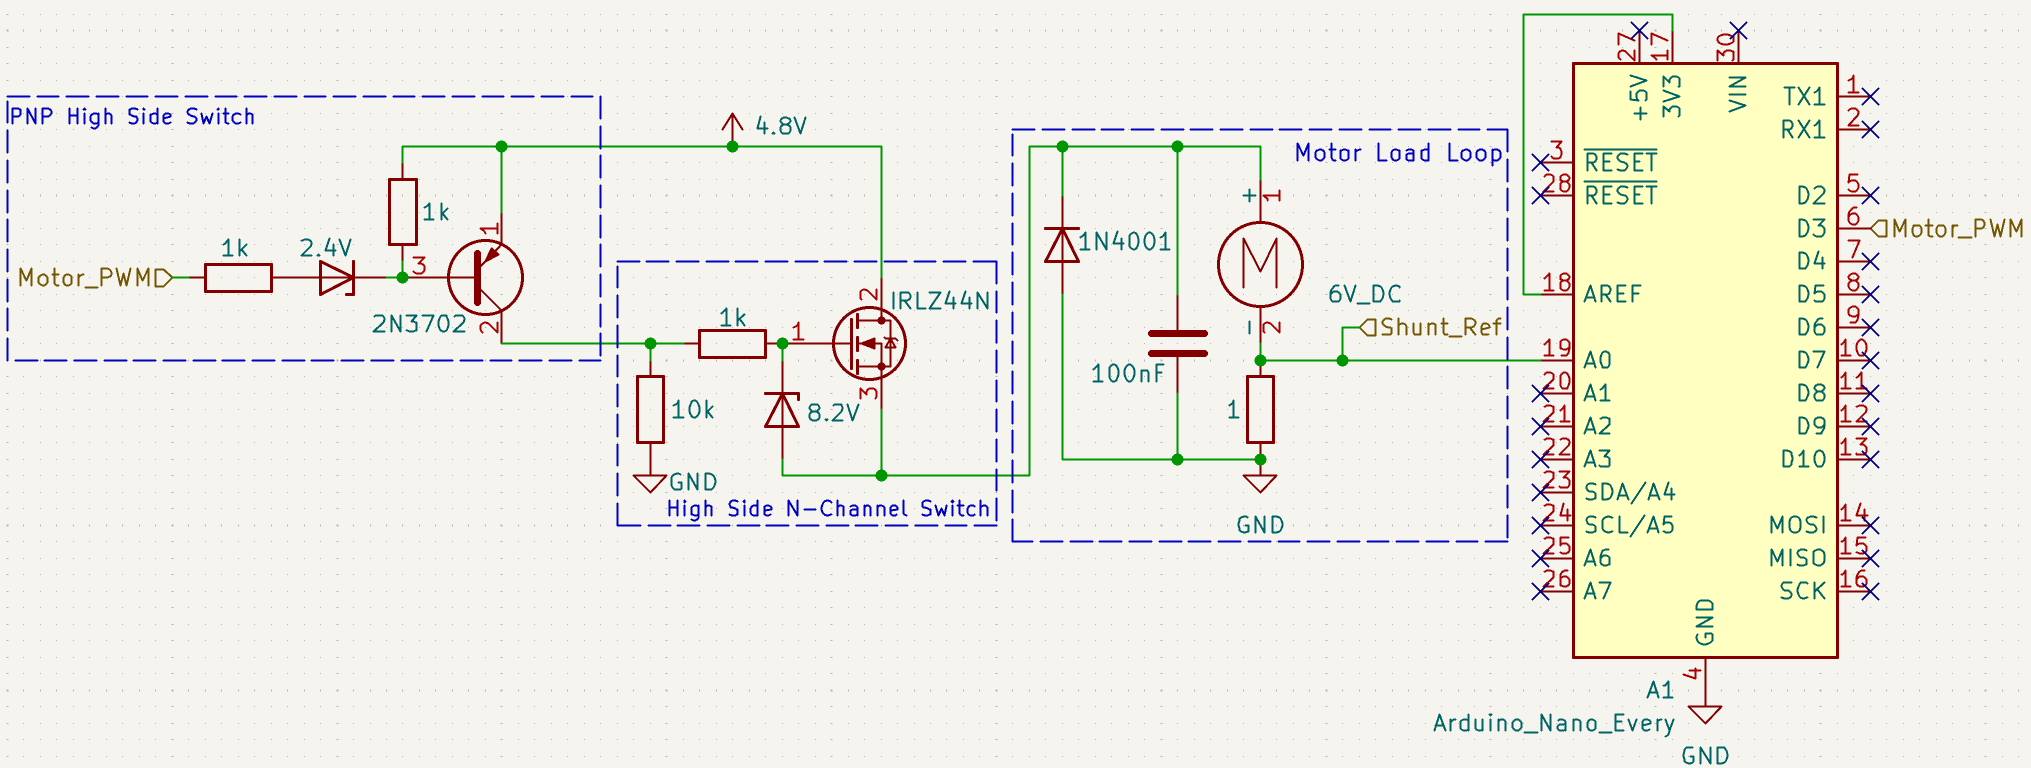
\includegraphics[width=1\linewidth]{circuits/motor_control.png}
    \caption[Design G: Schematic]{Schematic diagram of Design G; a High-side motor drive circuit with current sensing shunt resistor.}
\label{fig:high_side_motor}
\end{figure}

Design F was built on a standard RH-32 breadboard following the schematic in Fig.\ref{fig:high_side_motor}. Firstly, the PNP high side switch was assembled using a 2N3702 \cite{Components101_2N3702}; the emitter (pin 1) of the PNP transitor was connected to the \(4.8\) V DC supply rail,  a \(1\) k\(\Omega\) resistor was connected between the base (pin 3) of the transistor and the \(4.8\) V DC 3631A lab power supply rail. Next, the base clamping \(2.4\) V zener diode was connected with the cathode connecting to the 2N3702 base (pin 3) and on the anode was connected to a \(1\) k\(\Omega\) current limiting resistor.

Secondly, the high-side N-Channel switch was built (Fig.\ref{fig:high_side_motor}) utilising an IRLZ44N N-Channel MOSFET \cite{Infineon_IRLZ44N}; the gate (pin 1) was connected with a \(1\) k\(\Omega\) gate resitor to the collector of IRLZ44N (pin 2) and the drain (pin 2) was connected to the \(4.8\) V DC 3631A lab power supply rail. A gate clamping \(8.2\) V zener diode was connected with the anode connecting to the IRLZ44N source (pin 3) and the cathode directly to the gate. As the schematic shows, a final \(10\) k\(\Omega\) pull-down resistor was connected to GND.

Third, the motor loop circuit (Fig.\ref{fig:high_side_motor}) was assembled as previously described in section \ref{sec:low_side_motor}, with the following variations:
\begin{itemize}
    \item The current sensing shunt resistor was connected to the bottom of the motor, then to ground.
    \item The anode of the flyback diode and the capacitor were connected to GND instead of the drain of IRLZ44N.
    \item The top side of the motor was connected to the source of IRLZ44N and not to the \(4.8\) V DC supply rail.
\end{itemize}

Fourth, the Arduino Nano Every was placed into the breadboard over the central channel. The analogue pin was connected first with A0 connecting to the shunt resistor and motor node (`Shunt\_Ref'). The D3 pin (Motor\_PWM) was then connected to the current limiting resistor for the base of 2N3072 as seen in Fig.\ref{fig:high_side_motor}. Following on, the GND was connected to the Arduino and the \(+3.3\) V DC supply rail from the Arduino was connected to the analogue reference (AREF) pin of the Arduino.

Finally, the Arduino program designed for Design G (Appendix \ref{app:Arduino} Listing \ref{cod:current_1ref}) was reuploaded to the Arduino Nano Every.


\subsubsection{Testing}
The testing method for Design F followed the same procedure as outlined in Section \ref{sec:low_side_motor} including the secondary investigation, with the exception of varying the PWM from \(255\rightarrow128\), representing a duty cycle range of \(100\rightarrow50\%\). All measurements were taken under the same conditions and analysed accordingly as defined in \ref{sec:low_side_motor}.

\section{Results}
\subsection{Design F: Low-Side Motor Drive}

\begin{table}[H]
    \centering
    \caption[Design F: Current Measurements]{Design F measured current compared to Arduino current calculated values (Appendix \ref{app:data} Table \hyperref[tab:A.8]{A.8})}
    \label{tab:Low_current}
    \begin{tabular}{|c|c||c|c||c|}\hline
     &&\multicolumn{2}{|c||}{Current (A)} &  \\\hline
    PWM &Duty Cycle \%&Multi-meter Average&Arduino Average&Absolute Error \\ \hline 
    0 &0&0.001&0.00&-0.001\\ \hline
    8 &3.14&0.014&0.01&-0.004\\\hline
    16 &6.27&0.043&0.04&-0.003\\\hline
    24 &9.41&0.080&0.08&0.000\\\hline
    32 &12.55&0.113&0.12&0.007\\\hline
    40 &15.69&0.125&0.13&0.005\\\hline
    48 &18.82& 0.163& 0.16& -0.003\\\hline
    56 &21.96& 0.171& 0.17& -0.001\\\hline
    64 &25.1& 0.184& 0.18& -0.004\\\hline
    72 &28.24& 0.188& 0.19& 0.002\\\hline
    80 &31.37& 0.200& 0.20& 0.000\\\hline
    88 &34.51& 0.211& 0.21& -0.001\\\hline
    96 &37.65& 0.221& 0.22& -0.001\\\hline
    104 &40.78& 0.221& 0.21& -0.011\\\hline
    112 &43.92& 0.208& 0.21& 0.002\\\hline
    120 &47.06& 0.214& 0.22& 0.006\\\hline
    128 &50.2& 0.220& 0.22& 0.000\\\hline\end{tabular}  
\end{table}

\begin{table}[H]
    \centering
    \caption[Design F: Current Measurements]{Design F measured current compared to Arduino current calculated values with pressure applied to wheel (Appendix \ref{app:data} Table \hyperref[tab:A.9]{A.9})}
    \label{tab:Low_current_pressure}
    \begin{tabular}{|c|c||c|c||c|}\hline
     &&\multicolumn{2}{|c||}{Current (A)} &  \\\hline
    PWM &Duty Cycle \%&Multi-meter Average&Arduino Average&Absolute Error \\ \hline 
    24 &9.41&0.085&0.09&0.005\\ \hline
    56 &21.96&0.313&0.32&0.007\\\hline
    80 &31.37&0.508&0.51&0.002\\\hline
    104 &40.78&0.710&0.71&0.000\\\hline
    128 &50.2&0.992&0.99&-0.002\\\hline\end{tabular}  
\end{table}

The observed Arduino current values closely followed the multi-meter values (Tables \ref{tab:Low_current}, \ref{tab:Low_current_pressure}).

\begin{table}[H]
    \centering
    \caption[Design F: Voltage Measurements \(1\) k\(\Omega\) Resistor Load]{Design F measured voltage when the circuit load is a \(1\) k\(\Omega\) resistor (Appendix \ref{app:data} Table \hyperref[tab:A.10]{A.10}).}
    \label{tab:low_voltage_1k}
    \begin{tabular}{|c|c||c|c||c|}\hline
     &&\multicolumn{2}{|c||}{Voltage (V)} &  \\\hline
    PWM &Duty Cycle \%&Expected&Multi-meter Average&Absolute Error \\ \hline 
    0&0&0&0.000&0.000\\ \hline
    24&9.41&0.45&0.200&0.251\\\hline
    56&21.96&1.05&1.057&-0.003\\\hline
    80&31.37&1.51&1.500&0.006\\\hline
    104&40.78&1.96&1.958&-0.001\\\hline
 128& 50.2& 2.41& 2.410&0.000\\\hline\end{tabular}  
\end{table}

In Table \ref{tab:low_voltage_1k} the discrepancy between expected voltage and measured voltage at 9.4\% duty cycle may be caused by incorrect multi-meter averaging of short pulses. However, with the remaining data the measured and expected values closely agree.

\subsubsection{Cost of Implementation}

\begin{table}[H]
\centering
\caption{Alphabetically Ordered Estimated Component Costs for Design F}
\begin{tabular}{|l|c|c|c|}
\hline
\textbf{Component}                & \textbf{Quantity} & \textbf{Unit Price (£)} & \textbf{Total Price (£)}\\ \hline
100nF Polyester Capacitor\cite{rs_100nfcap_poly} & 1 & 0.486 & 0.486\\ \hline
10kΩ Resistor \cite{rs_10kresistor} & 1 & 0.07 & 0.07\\ \hline
1Ω Resistor \cite{rs_res1}& 1 & 0.162 & 0.162\\ \hline
1N4001 Diode \cite{rs_1n4001} & 1 & 0.103 & 0.103\\ \hline
NiMH 1.2V AA Batteries \cite{rs_nimh} & 4 & 2.243 & 8.972\\ \hline
IRLZ44N N-Channel MOSFET \cite{rs_irlz44n} & 1 & 0.717 & 0.717\\ \hline\hline
\textbf{Total Estimated Cost} &&&\textbf{£10.51}\\ \hline
\end{tabular}
\label{tab:cost_designf}
\end{table}

Table \ref{tab:cost_designf} details the individual components required for the implementation of Design F, alongside their quantities, specifications, suppliers, and unit costs based on UK-sourced pricing at the time of writing. The cost of implementation within the `mouse' would be £12.05, adding a second version of the design without additional NiMH batteries. The cost difference between the original sub-system (Appendix \ref{app:mouseecost_og}) is +£1.57 an increase in cost of \(15\%\).
\newpage
\subsection{Design G: High-Side Motor Drive}

Please note, as mentioned in section \ref{sec:highside}, the PWM and duty cycle values are inverted.

\begin{table}[H]
    \centering
    \caption[Design G: Current Measurements]{Design G measured current compared to Arduino current calculated values (Appendix \ref{app:data} Table \hyperref[tab:A.11]{A.11})}
    \label{tab:High_current}
    \begin{tabular}{|c|c||c|c||c|}\hline
     &&\multicolumn{2}{|c||}{Current (A)} &  \\\hline
    PWM &Duty Cycle \%&Multi-meter Average&Arduino Average&Absolute Error \\ \hline 
    255 &100&0.001&0.00&-0.001\\ \hline
    247 &96.86&0.012&0.03&0.018\\\hline
    239 &93.73&0.026&0.04&0.014\\\hline
    231 &90.59&0.046&0.06&0.014\\\hline
    223 &87.45&0.069&0.09&0.021\\\hline
    215 &84.31&0.096&0.13&0.034\\\hline
    207 &81.18& 0.117& 0.17& 0.053\\\hline
    199 &78.04& 0.131& 0.14& 0.009\\\hline
    191 &74.9& 0.145& 0.18& 0.035\\\hline
    183 &71.76& 0.155& 0.18& 0.025\\\hline
    175 &68.63& 0.159& 0.18& 0.021\\\hline
    167 &65.49& 0.168& 0.20& 0.032\\\hline
    159 &62.35& 0.221& 0.18& -0.041\\\hline
    151 &59.22& 0.221& 0.19& -0.031\\\hline
    143 &56.08& 0.208& 0.21& 0.002\\\hline
    135 &52.94& 0.214& 0.19& -0.024\\\hline
    127 &49.8& 0.220& 0.22& 0.000\\\hline\end{tabular}  
\end{table}

\begin{table}[H]
    \centering
    \caption[Design G: Current Measurements]{Design G measured current compared to Arduino current calculated values with pressure applied to wheel (Appendix \ref{app:data} Table \hyperref[tab:A.12]{A.12})}
    \label{tab:High_current_pressure}
    \begin{tabular}{|c|c||c|c||c|}\hline
     &&\multicolumn{2}{|c||}{Current (A)} &  \\\hline
    PWM &Duty Cycle \%&Multi-meter Average&Arduino Average&Absolute Error \\ \hline 
    231 &90.59&0.049&0.07&0.021\\ \hline
    207 &81.18&0.131&0.20&0.069\\\hline
    183 &71.76&0.238&0.29&0.052\\\hline
    159 &62.35&0.313&0.40&0.087\\\hline
    127 &49.8&0.472&0.56&0.088\\\hline\end{tabular}  
\end{table}

The observed Arduino current values are in the same order as the multi-meter values but are not close matches (Tables \ref{tab:High_current}, \ref{tab:High_current_pressure}).

\begin{table}[H]
    \centering
    \caption[Design G: Voltage Measurements \(1\) k\(\Omega\) Resistor Load]{Design G measured voltage when the circuit load is a \(1\) k\(\Omega\) resistor (Appendix \ref{app:data} Table \hyperref[tab:A.13]{A.13}).}
    \label{tab:high_voltage_1k}
    \begin{tabular}{|c|c||c|c||c|}\hline
     &&\multicolumn{2}{|c||}{Voltage (V)} &  \\\hline
    PWM &Duty Cycle \%&Expected&Multi-meter Average&Absolute Error \\ \hline 
    255&100&0&0.000&0.000\\ \hline
    231&90.59&0.45&0.194&0.257\\\hline
    207&81.18&0.9&0.319&0.584\\\hline
    183&71.76&1.36&0.931&0.425\\\hline
    159&62.35&1.81&1.151&0.656\\\hline
 127& 49.8& 2.41& 1.534&0.876\\\hline\end{tabular}  
\end{table}

The values seen in Table \ref{tab:high_voltage_1k} demonstrate a linear relationship between PWM and multi-meter voltage. However, the values measured are significantly lower than expected, particularly at lower duty cycles.


\subsubsection{Cost of Implementation}

\begin{table}[H]
\centering
\caption{Alphabetically Ordered Estimated Component Costs for Design G}
\begin{tabular}{|l|c|c|c|}
\hline
\textbf{Component}                & \textbf{Quantity} & \textbf{Unit Price (£)} & \textbf{Total Price (£)}\\ \hline
100nF Polyester Capacitor\cite{rs_100nfcap_poly} & 1 & 0.486 & 0.486\\ \hline
10kΩ Resistor \cite{rs_10kresistor} & 1 & 0.07 & 0.07\\ \hline
1kΩ Resistor \cite{rs_1kresistor} & 1 & 0.162 & 0.486\\ \hline
1Ω Resistor \cite{rs_res1}& 1 & 0.162 & 0.162\\ \hline
1N4001 Diode \cite{rs_1n4001} & 1 & 0.103 & 0.103\\ \hline
2.4V Zener Diode \cite{rs_24vzdiode} & 1 & 0.129 & 0.129\\ \hline
8.2V Zener Diode \cite{rs_82vzdiode} & 1 & 0.117 & 0.117\\ \hline
NiMH 1.2V AA Batteries \cite{rs_nimh} & 4 & 2.243 & 8.972\\ \hline
IRLZ44N N-Channel MOSFET \cite{rs_irlz44n} & 1 & 0.717 & 0.717\\ \hline\hline
\textbf{Total Estimated Cost} &&&\textbf{£11.24}\\ \hline
\end{tabular}
\label{tab:cost_designg}
\end{table}

Table \ref{tab:cost_designg} details the individual components required for the implementation of Design G, alongside their quantities, specifications, suppliers, and unit costs based on UK-sourced pricing at the time of writing. The cost of implementation within the `mouse' would be £13.51, adding a second version of the design without additional NiMH batteries. The cost difference between the original sub-system (Appendix \ref{app:mouseecost_og}) is +£3.03 an increase in cost of \(28\%\).

\section{Discussion}
This section evaluates two design solutions proposed to facilitate the addition of a current feedback system to improve the control loop currently implemented in the `mouse' design. Firstly, of the two designs considered, the low-side design is superior in both performance and cost effectiveness. Secondly, whilst not the focus of this section, the back EMF voltage caused by the motor directly impacts the PWM performance of the motor drive circuit. Directly driving the motor with a PWM drive signal increases undesirable EMI noise due to fast transitions and inductive loads; good layout and screening are recommended. 

Before further interpreting the findings, it is essential to acknowledge several key limitations. Firstly, no precise method for pressure application was used when testing the current observed in the motor. Conversely, the aim of the current test wasn't to ascertain the exact pressure to achieve a certain motor current but to investigate the current observation method and its accuracy in relation to varying values. Secondly, for consistency of results the \(4.8\) V power rail in Design G and F was provided with a laboratory power supply and not batteries, which will have a higher impedance especially as they discharge with use potentially impacting performance. Third, the performance of the designs may have been slightly impacted by the use of the RH-32 breadboard, introducing additional contact impedance.

\subsubsection{Design Performance}
The motor PWM response in Design F was accurate, and the current sensing addition gave an accurate representation of the current; this fulfils the requirements described in section \ref{sec:overview_motor}. In contrast, Design G was adequate but inferior to Design F in both current sensing and PWM control.

\subsubsection{Complexity}
Design F is significantly easier to introduce, only requiring minor modification and simple electrical engineering concepts when compared to the current motor drive methods. In contrast, Design G requires extra components and requires high-level understanding of transistor and MOSFET behaviour.

\subsubsection{Cost}
Comparing the cost of implementation, it is clear that Design F is superior as it only introduces the cost estimate of £2.20 compared to Design Gs cost of £3.03, a difference of £0.81. It should be noted that some of these cost differences when compared to the design seen in \cite{Noah2023} have arisen from the different choices in MOSFET or transistor, as well as the choice of motor transient reduction components; therefore, the values seen should be noted as estimates and not accurate representations of true cost per `mouse'.
 
\subsubsection{Further Investigations}
Further investigation should be conducted on integrating Design F into a working `mouse', developing appropriate software to integrate the motor current measurement into the overall control loop. In addition, a potential investigation of a reduction in the shunt resistor value to \(\approx0.5\) \(\Omega\) could be valuable in terms of extra power potential within the motor, this may involve the introduction of an amplifier or utilising the \(1.1\) V internal Arduino \cite{Microchip_ATmega4809, Arduino_Every} voltage reference.

\subsubsection{Recommendations}
Overall, Design F is clearly the most appropriate option when considering the addition of current sensing within the motor, adding reliable data that can be utilised in improvements to `mouse' control loop.

\chapter{Overall Discussion and Conclusions}
Please see the discussion and conclusions of each sub-project named in Table \ref{tab:letterciruit_def} (A to G). As previously stated, my recommendations for circuit designs to be included in the `mouse' project going forward are designs B, D and F. In the sub-system sections, specific suggestions have been made regarding future development and project work.

While carrying out the project an additional idea for future project work is to investigate the complete removal of the 9 V alkaline batteries and instead power the entire mouse from 5 x NiMH rechargeable AA batteries. In this configuration, the Arduino would be powered from the AA batteries and supply the voltage required for the operational amplifiers within the position feedback sub-system. 

In conclusion, the aims and objectives of this project have been successfully completed.

{\let\clearpage\relax\chapter{Project Review}}
While the results of the sub-projects are mixed, this has not impacted the overall success of the project with three designs recommended that meet the project objectives defined in section \ref{sec:aims&obj}. The designs suggested were reached after various testing methods and are believed to be the most appropriate circuits to facilitate the reduction in batteries and the addition of feedback to the control loop. Observations and testing conducted during the project have deepened the understanding of the mouse limitations and its potential for further investigation and improvement.

I encountered various issues throughout the project, ranging from testing to component malfunction. Each sub-project section discusses the specific testing issues I encountered. However, one recurring issue encountered during testing was the death of 5 Arduino Nanos, a big setback that knocked my confidence and delayed further tests. I was able to fix this problem by rebuilding my circuits on a separate breadboard, suggesting that the issue lay with the breadboard and not my design.

With hindsight, I would focus on one sub-system at a time, as trying to develop three sub-systems in conjunction leads to mistakes being made in circuit prototyping and missing out on further potential improvements. However, this does not override the positives mentioned previously and hence the project should be classed as a success. 

{\let\clearpage\relax\chapter{Acknowledgment}}
\section{Personal Acknowledgment}
I wish to thank my supervisor, Dr. Francis Robinson, for guiding me through this project and putting up with my endless questions and queries. Additionally, I would like to thank the lab technicians, Richmond Afeawo and Chun JW Wong, who helped me during testing and integration. I would also like to thank Alasdair Philips, who advised me on various topics during testing and the write-up. Lastly, I would like to acknowledge my partner, Bee, who has helped keep me motivated and has been my rock during this project.

\section{AI Acknowledgment}
All statements are based of the suggestions seen in \cite{Rowland_2023}.

I acknowledge that ChatGPT was used to identify themes in the notes I took from the sources I found. I then grouped and organised these themes into a logical order myself and used or adapted some of the themes' phrasing in my topic sentences.

I acknowledge that the Pro version of Grammarly was used to correct grammatical and punctuation errors, and to make minor refinements to my draft text. I reviewed the results and take full responsibility for the content of the assignment.







\newcommand{\BIBdecl}{\setlength{\itemsep}{0.25 em}\addcontentsline{toc}{chapter}{Bibliography}}
\bibliographystyle{IEEEtran}
\bibliography{references}





\appendix
\chapter{Appendices}
\section{Project Costs}

\begin{table}[H]
\centering
\caption{Total Project Costs}
\label{tab:cots_tot}
\begin{tabular}{|l ||l |l |l|} \hline 
\textbf{Item} & \textbf{Quantity} & \textbf{Cost} & \textbf{Total Cost} \\ \hline 
100nF Ceramic Disc Capacitor (50V) & 7 & £0.17 & £1.19 \\ \hline 
100nF Polyester Capacitor & 2 & £0.49 & £0.97 \\ \hline 
10kΩ Through-Hole Resistor & 3 & £0.07 & £0.21 \\ \hline 
10nF Polyester Capacitor & 1 & £0.11 & £0.11 \\ \hline 
1kΩ Resistor & 7 & £0.16 & £1.13 \\ \hline 
1N4001 Diode & 2 & £0.10 & £0.21 \\ \hline 
1N4148 Signal Diode & 2 & £0.01 & £0.02 \\ \hline 
1μF Electrolytic Capacitor & 1 & £0.22 & £0.22 \\ \hline 
1Ω Resistor & 10 & £0.16 & £1.62 \\ \hline 
2.2nF Ceramic Capacitor & 1 & £0.07 & £0.07 \\ \hline 
2.4V Zener Diode & 1 & £0.13 & £0.13 \\ \hline 
33nF Capacitor (Polyester, 100V) & 2 & £0.12 & £0.24 \\ \hline 
4.7μF Electrolytic Capacitor & 1 & £0.21 & £0.21 \\ \hline 
47kΩ Resistor  & 1 & £0.17 & £0.17 \\ \hline 
5.6kΩ Resistor & 1 & £0.11 & £0.11 \\ \hline 
51kΩ Resistor & 2 & £0.05 & £0.11 \\ \hline 
8.2V Zener Diode & 1 & £0.12 & £0.12 \\ \hline 
9V Battery (RS PRO Alkaline) & 1 & £2.08 & £2.08 \\ \hline 
Allegro Microsystems Through Hole Hall Effect Sensor & 5 & £0.61 & £3.05 \\ \hline 
Arduino Nano Every & 9 & £11.55 & £103.95 \\ \hline 
IRLZ44N N-Channel MOSFET & 4 & £0.72 & £2.87 \\ \hline 
NE555P Timer IC & 1 & £0.15 & £0.15 \\ \hline 
NiMH 1.2V AA Batteries & 4 & £2.24 & £8.97 \\ \hline 
RS PRO Neodymium Magnet 0.09kg, Width 3mm. & 1 & £4.69 & £4.69 \\ \hline 
RS PRO Tachometer Reflective Tape. & 1 & £8.24 & £8.24 \\ \hline 
Single Core Wire (Various Lengths) & 1 & £15.00 & £15.00 \\ \hline 
TCRT5000 Module Switch Electronics & 4 & £1.37 & £5.48 \\ \hline 
TL071 Op-Amp (Single BiFET) & 2 & £0.45 & £0.90 \\\hline\hline
\textbf{Total Project Cost} &  &  & \textbf{£162.21} \\ \hline

\end{tabular}

\end{table}

Table \ref{tab:cots_tot} details the total project costs; items such as battery cradles and breadboard jumper wires have not been included due to them being borrowed and returned to EEE stores. I estimate the time contribution from Lab Technicians to be 2 hours. 

\newpage
\section{Original Sub-System Estimated Cost}
\label{app:mouseecost_og}
\begin{table}[H]
    \centering
    \caption[Estimated Cost of Position Feedback Sub-System ]{Estimated cost of position feedback sub-system without LC filter, adapted from the circuit and cost appendix seen in \cite{Noah2023}.}
    \begin{tabular}{|l|c|c|c|}
    \hline
    \textbf{Component} & \textbf{Quantity} & \textbf{Unit Price (£)} & \textbf{Total Price (£)}\\ \hline
    33nF Capacitor & 2 & 0.12 & 0.24\\ \hline
    100nF Capacitor & 2 & 0.17 & 0.34\\ \hline
    TL071 OpAmp & 2 & 0.45 & 0.90\\ \hline
    1N4148 Signal Diode & 4 & 0.01 & 0.04\\ \hline
    4.7kΩ Resistor & 2 & 0.02 & 0.04\\ \hline
    470kΩ Potentiometer & 2 & 0.85 & 1.70\\ \hline
    9V Batteries & 2 & 2.08 & 4.16\\ \hline\hline
    \textbf{Total Estimated Cost} &&& \textbf{£7.38}\\ \hline
    \end{tabular}
\end{table}
\begin{table}[H]
    \centering
    \caption[Estimated Cost of Motor Drive Sub-System ]{Estimated cost of motor drive sub-system, adapted from the circuit and cost appendix seen in \cite{Noah2023}.}
    \begin{tabular}{|l|c|c|c|}
    \hline
    \textbf{Component} & \textbf{Quantity} & \textbf{Unit Price (£)} & \textbf{Total Price (£)}\\ \hline
    100nF Capacitor & 2 & 0.486 & 0.972\\ \hline
    1N4148 Signal Diode & 2 & 0.01 & 0.02\\ \hline
    TIP120 & 2 & 0.26 & 0.52\\ \hline
    NiMH 1.2V AA Batteries & 4 & 2.243 & 8.972\\ \hline\hline
    \textbf{Total Estimated Cost} &&& \textbf{£10.48}\\ \hline
    \end{tabular}
\end{table}

\newpage
\section{Arduino Program Code}
\label{app:Arduino}
\lstinputlisting[language=C,caption={RPM Calculation utilising interupts on the Arduino Nano Every},label=cod:RPM]{code/feedback.ino}
\indent\makebox[\linewidth]{\rule{0.8\paperwidth}{0.4pt}}
\lstinputlisting[language=C,caption={Current Calulation using One Refernce point Arduino Nano Every},label=cod:current_1ref]{code/current2.ino}

\section{Equipment and Testing}
\label{app:equip&test}

\begin{figure}[H]
    \centering
    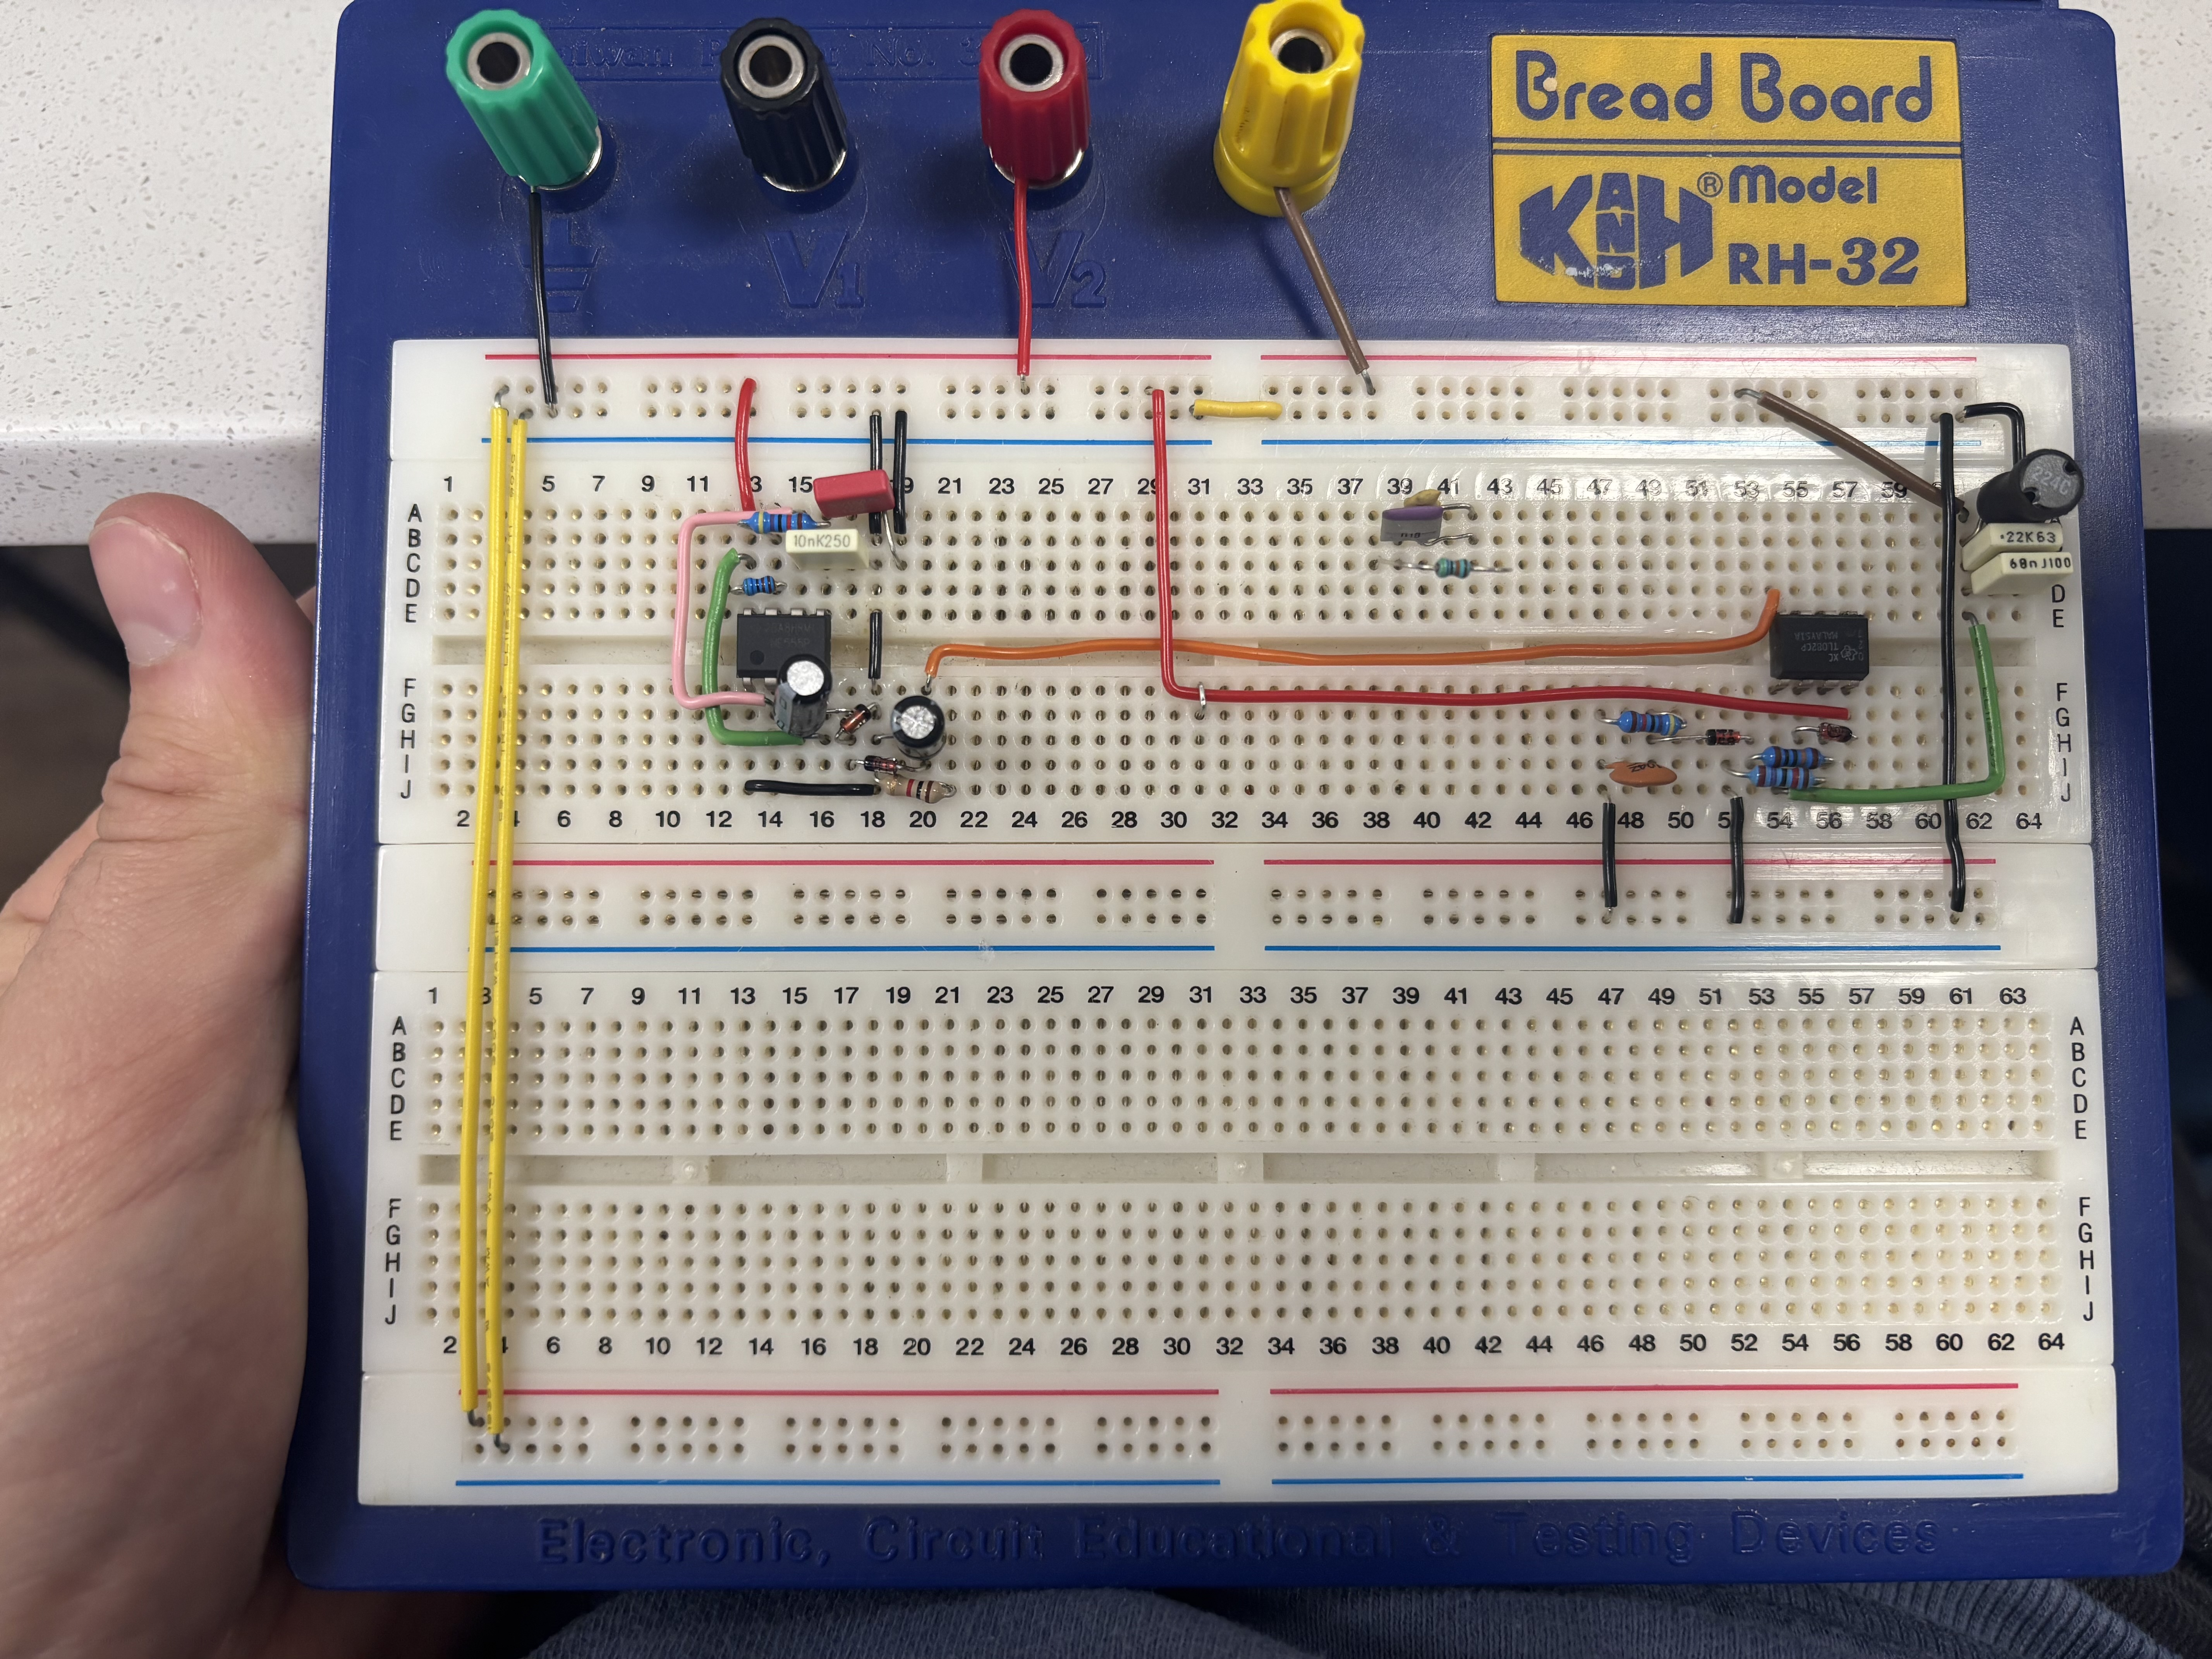
\includegraphics[width=0.75\linewidth,]{photos/rh32.jpg}
    \caption{RH-32 Breadboard}
    \label{fig:bread}
\end{figure}

\begin{figure}[H]
    \centering
    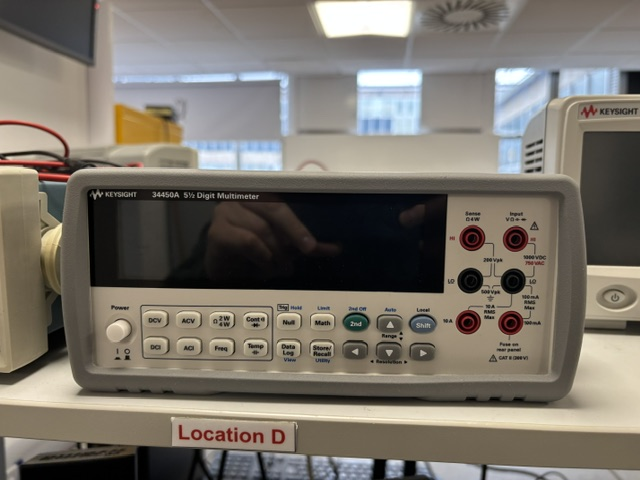
\includegraphics[width=0.75\linewidth]{photos/multi.jpeg}
    \caption{34450A KeySight Multi-meter}
    \label{fig:multi_m}
\end{figure}

\begin{figure}[H]
    \centering
    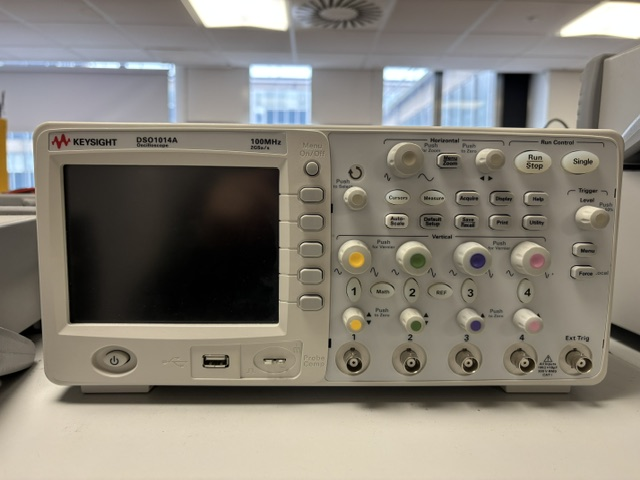
\includegraphics[width=0.75\linewidth]{photos/oscill.jpeg}
    \caption{DSO1014A Oscilloscope}
    \label{fig:osc}
\end{figure}

\begin{figure}[H]
    \centering
    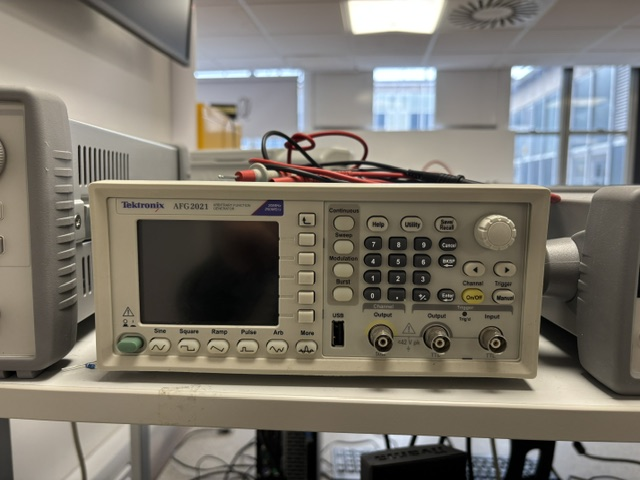
\includegraphics[width=0.75\linewidth]{photos/signal.jpeg}
    \caption{AFG2021 Signal Generator}
    \label{fig:signalgen}
\end{figure}

\begin{figure}[H]
    \centering
    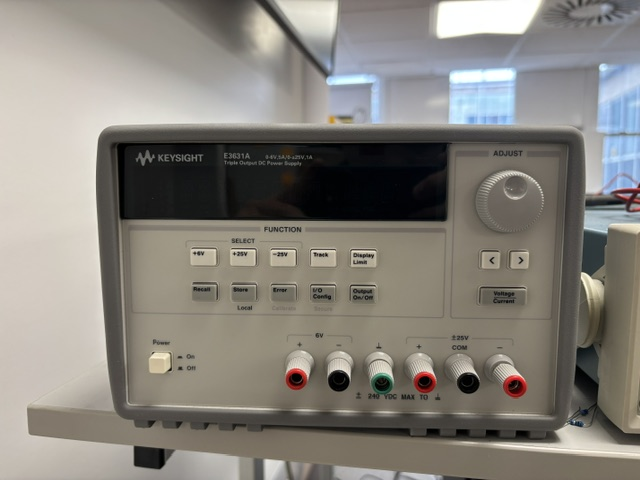
\includegraphics[width=0.75\linewidth]{photos/powersupply.jpeg}
    \caption{Lab KeySight E3631A DC Power supply}
    \label{fig:power_sup}
\end{figure}

\begin{figure}[H]
    \centering
    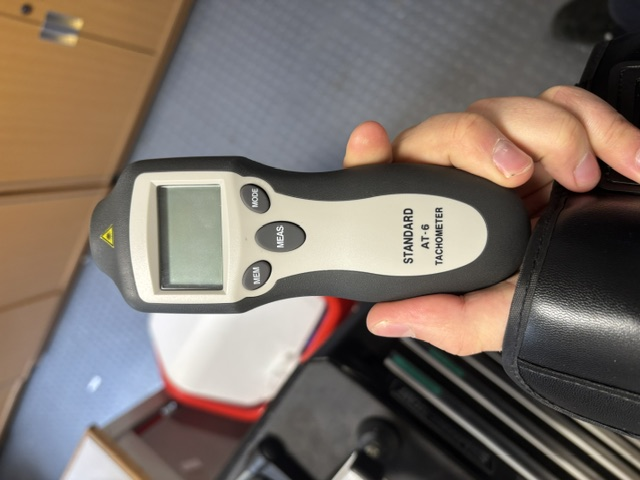
\includegraphics[width=0.75\linewidth, angle= -90]{photos/tach.jpeg}
    \caption{AT-6 Tachometer}
    \label{fig:tach}
\end{figure}

\newpage
\begin{figure}[H]
    \centering
    \begin{subfigure}{0.48\textwidth}
        \centering
        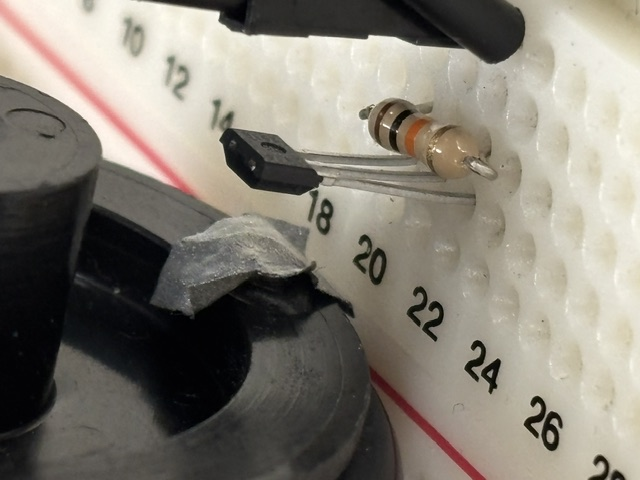
\includegraphics[width=\linewidth, angle=-90]{photos/hesang1.jpeg}
        \caption{HES Distance Angle 1}
        \label{fig:hes_ang1}
    \end{subfigure}\hfill
    \begin{subfigure}{0.48\textwidth}
        \centering
        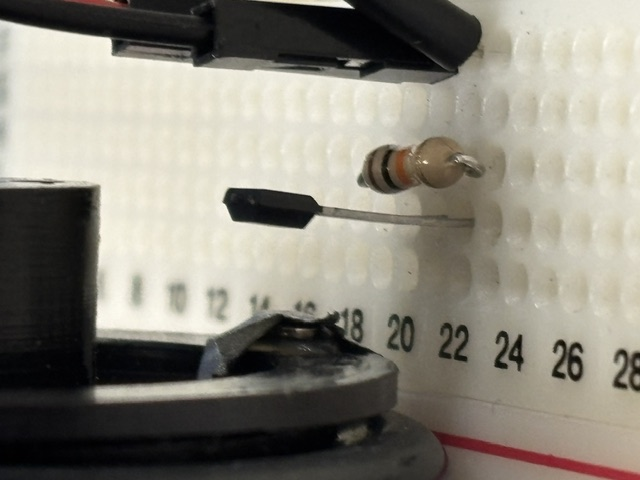
\includegraphics[width=\linewidth, angle=-90]{photos/hesang2.jpeg}
        \caption{HES Distance Angle 2}
        \label{fig:hes_ang2}
    \end{subfigure}
    \caption{Hall-Effect Sensor Distance at Different Angles}
    \label{fig:hes_distance_measurements}
\end{figure}

\begin{figure}[H]
    \begin{subfigure}{0.48\textwidth}
        \centering
        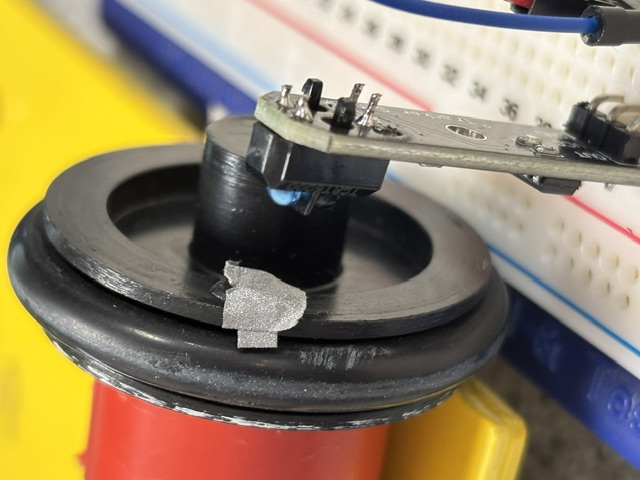
\includegraphics[width=\linewidth, angle=-90]{photos/optang1.jpeg}
        \caption{Optical Distance Angle 1}
        \label{fig:opt_ang1}
    \end{subfigure}\hfill
    \begin{subfigure}{0.48\textwidth}
        \centering
        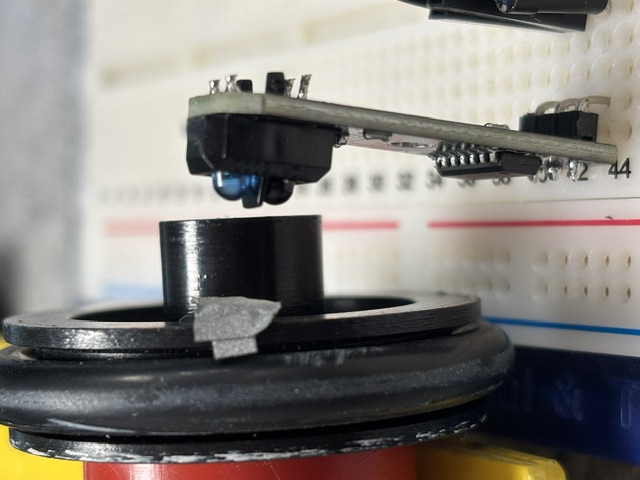
\includegraphics[width=\linewidth, angle=-90]{photos/optang2.jpeg}
        \caption{Optical Distance Angle 2}
        \label{fig:opt_ang2}
    \end{subfigure}
    \caption{Optical Sensor Distance at Different Angles}
    \label{fig:opt_distance_measurements}
\end{figure}


\section{Data}
\label{app:data}
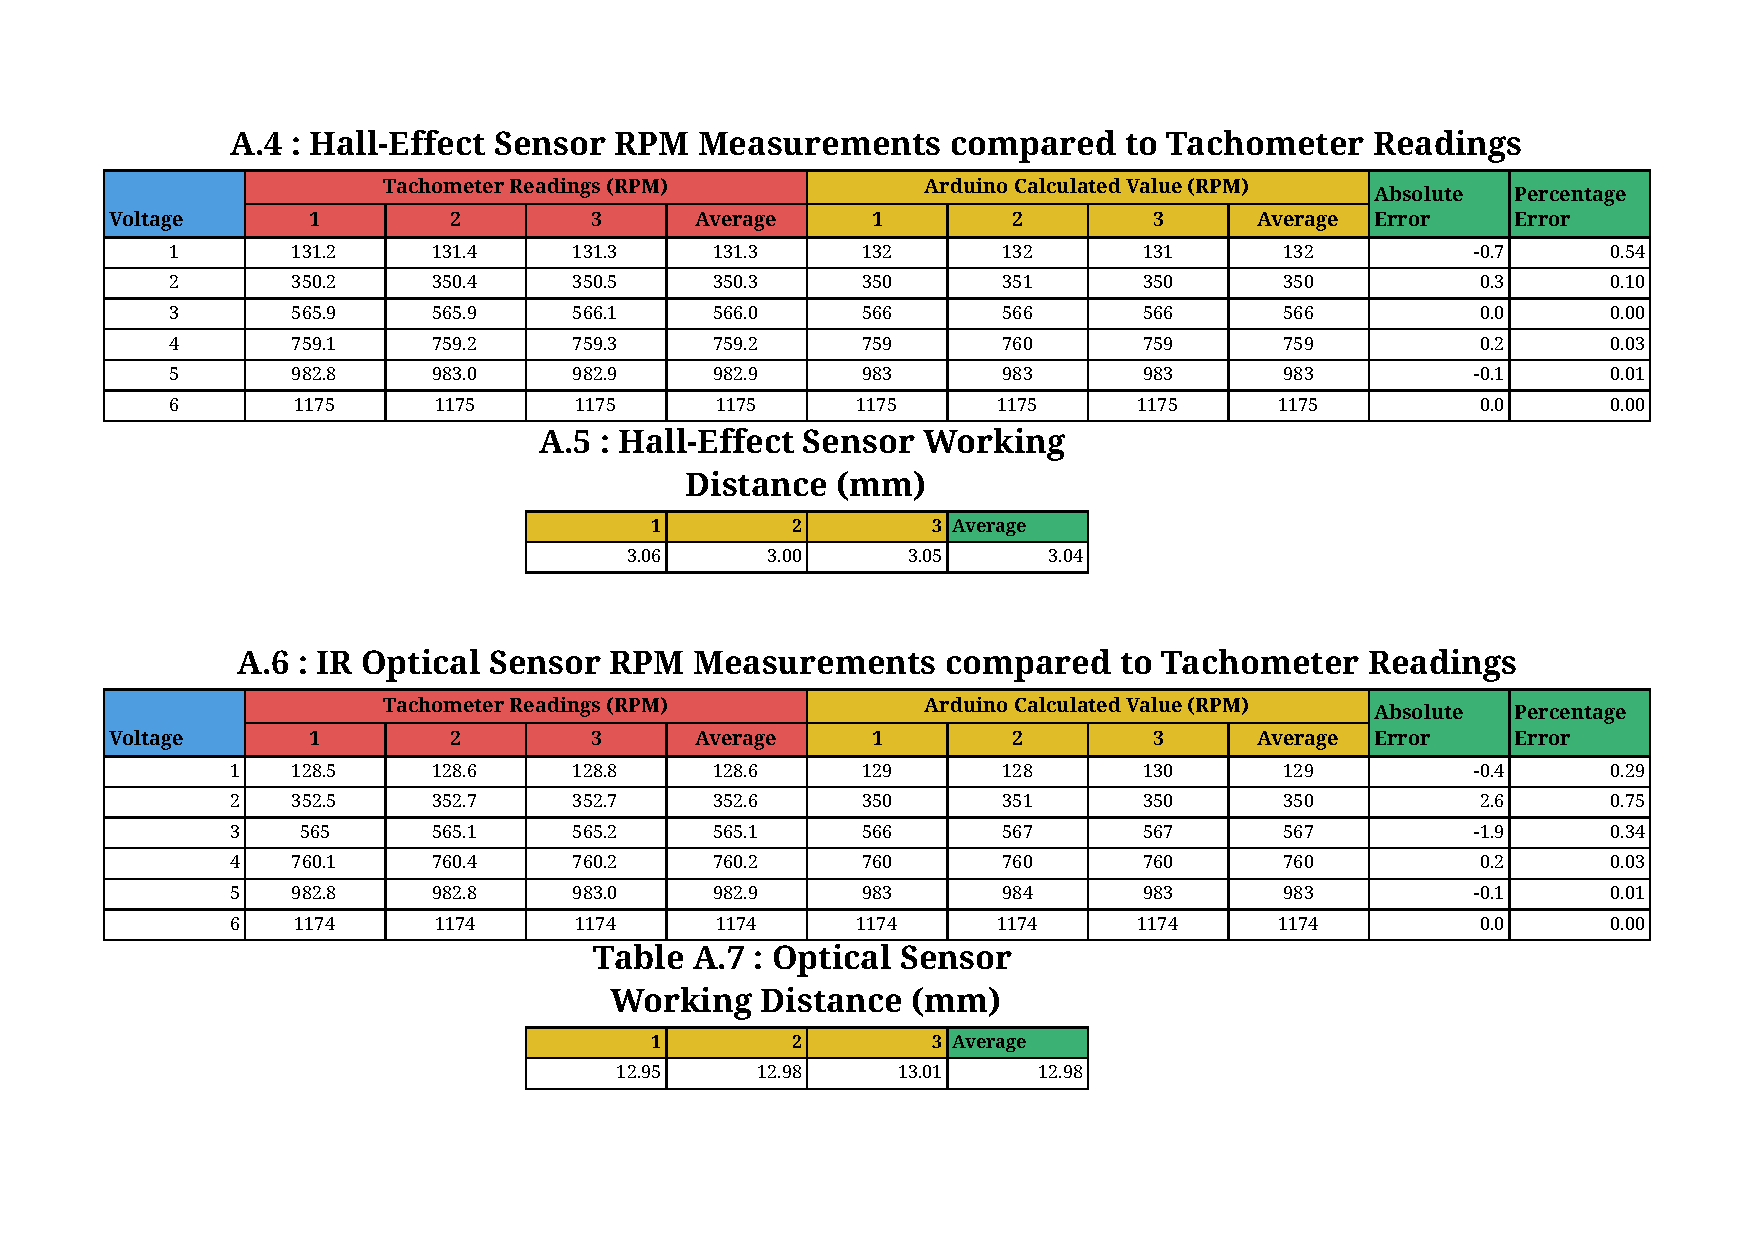
\includepdf[pages=1,landscape=true]{appendix data/Collation - RPM.pdf}
\addcontentsline{lot}{table}{A.4\hspace{0.5em}Hall-Effect Sensor and Tachometer RPM Readings}
\label{tab:A.4}
\addcontentsline{lot}{table}{A.5\hspace{0.5em}Hall-Effect Sensor Working Distance}
\label{tab:A.5}
\addcontentsline{lot}{table}{A.6\hspace{0.5em}Optical Sensor and Tachometer RPM Readings}
\label{tab:A.6}
\addcontentsline{lot}{table}{A.7\hspace{0.5em}Optical Sensor Sensor Working Distance}
\label{tab:A.7}
\begin{figure}[H]
    \centering
    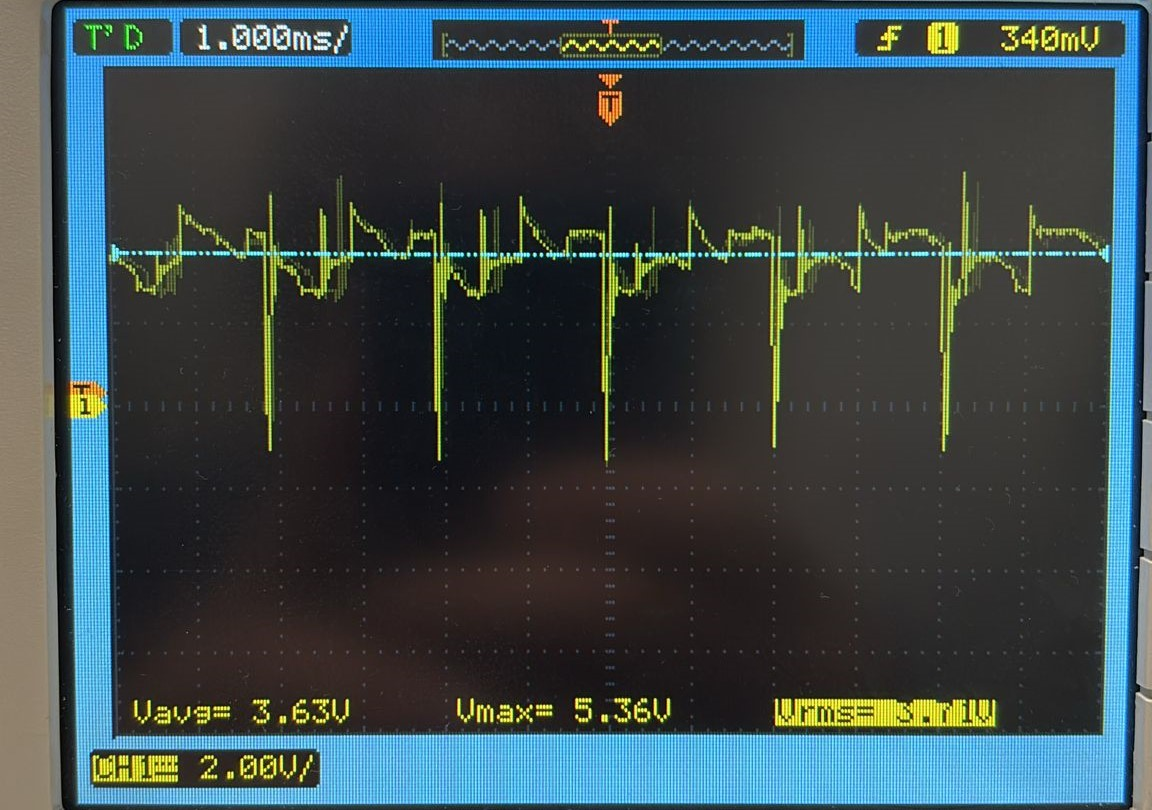
\includegraphics[width=1\linewidth]{photos/WhatsApp Image 2025-05-07 at 12.31.21.jpeg}
    \caption[Motor Back EMF Oscilloscope]{Oscilloscope response over the motor at 50\% duty cycle, demonstrating the issues encountered with back EMF from the motor.}
    \label{fig:osc_emf}
\end{figure}

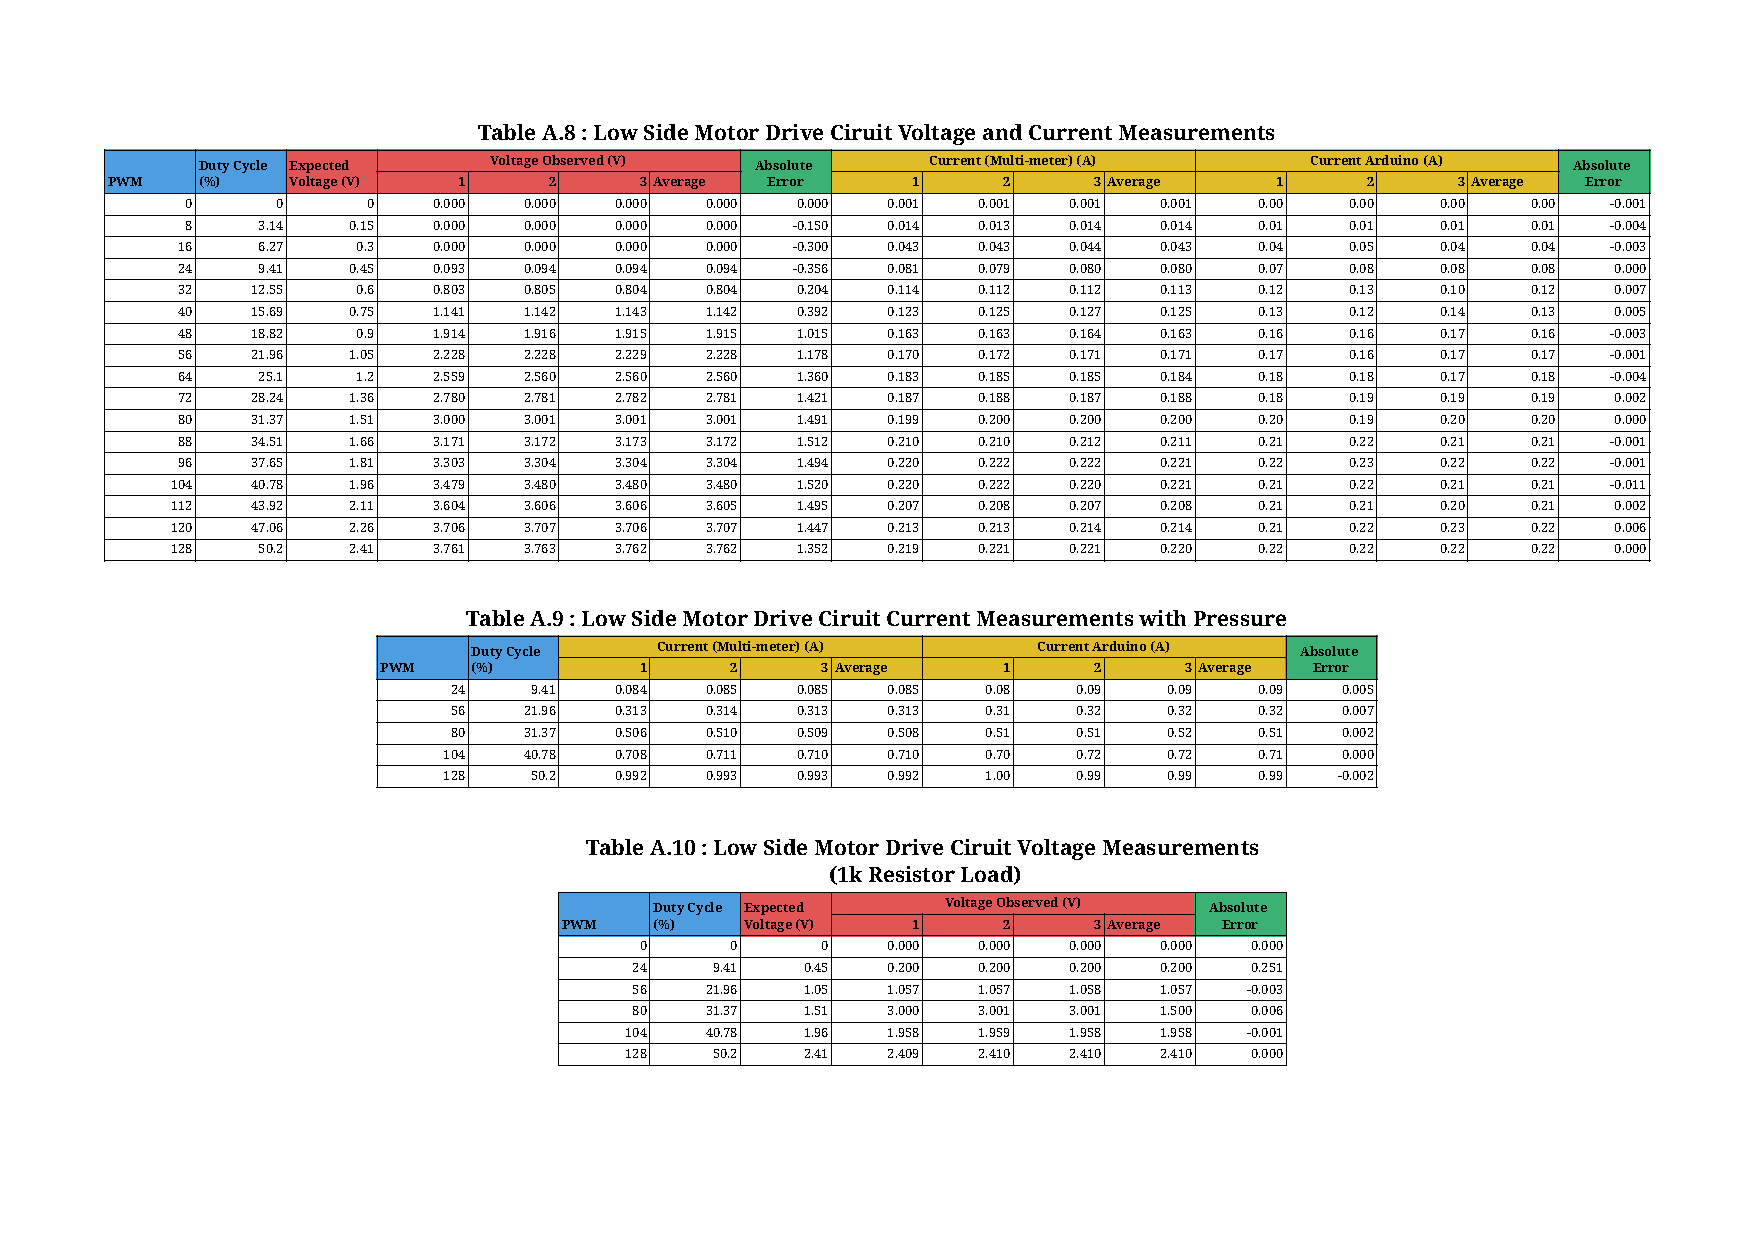
\includepdf[pages=-,landscape=true]{appendix data/Collation - LowSide.pdf}
\addcontentsline{lot}{table}{A.8\hspace{0.5em}Low Side Current and Voltage Measurements}
\label{tab:A.8}
\addcontentsline{lot}{table}{A.9\hspace{0.5em}Low Side Current Measurements with pressure}
\label{tab:A.9}
\addcontentsline{lot}{table}{A.10\hspace{0.5em}Low Side Voltage Measurements with 1 k\(\Omega\) resistor}
\label{tab:A.10}
\addcontentsline{lot}{table}{A.11\hspace{0.5em}High Side Current and Voltage Measurements}
\label{tab:A.11}
\addcontentsline{lot}{table}{A.12\hspace{0.5em}High Side Current Measurements with pressure}
\label{tab:A.12}
\addcontentsline{lot}{table}{A.13\hspace{0.5em}High Side Voltage Measurements with 1 k\(\Omega\) resistor}
\label{tab:A.13}

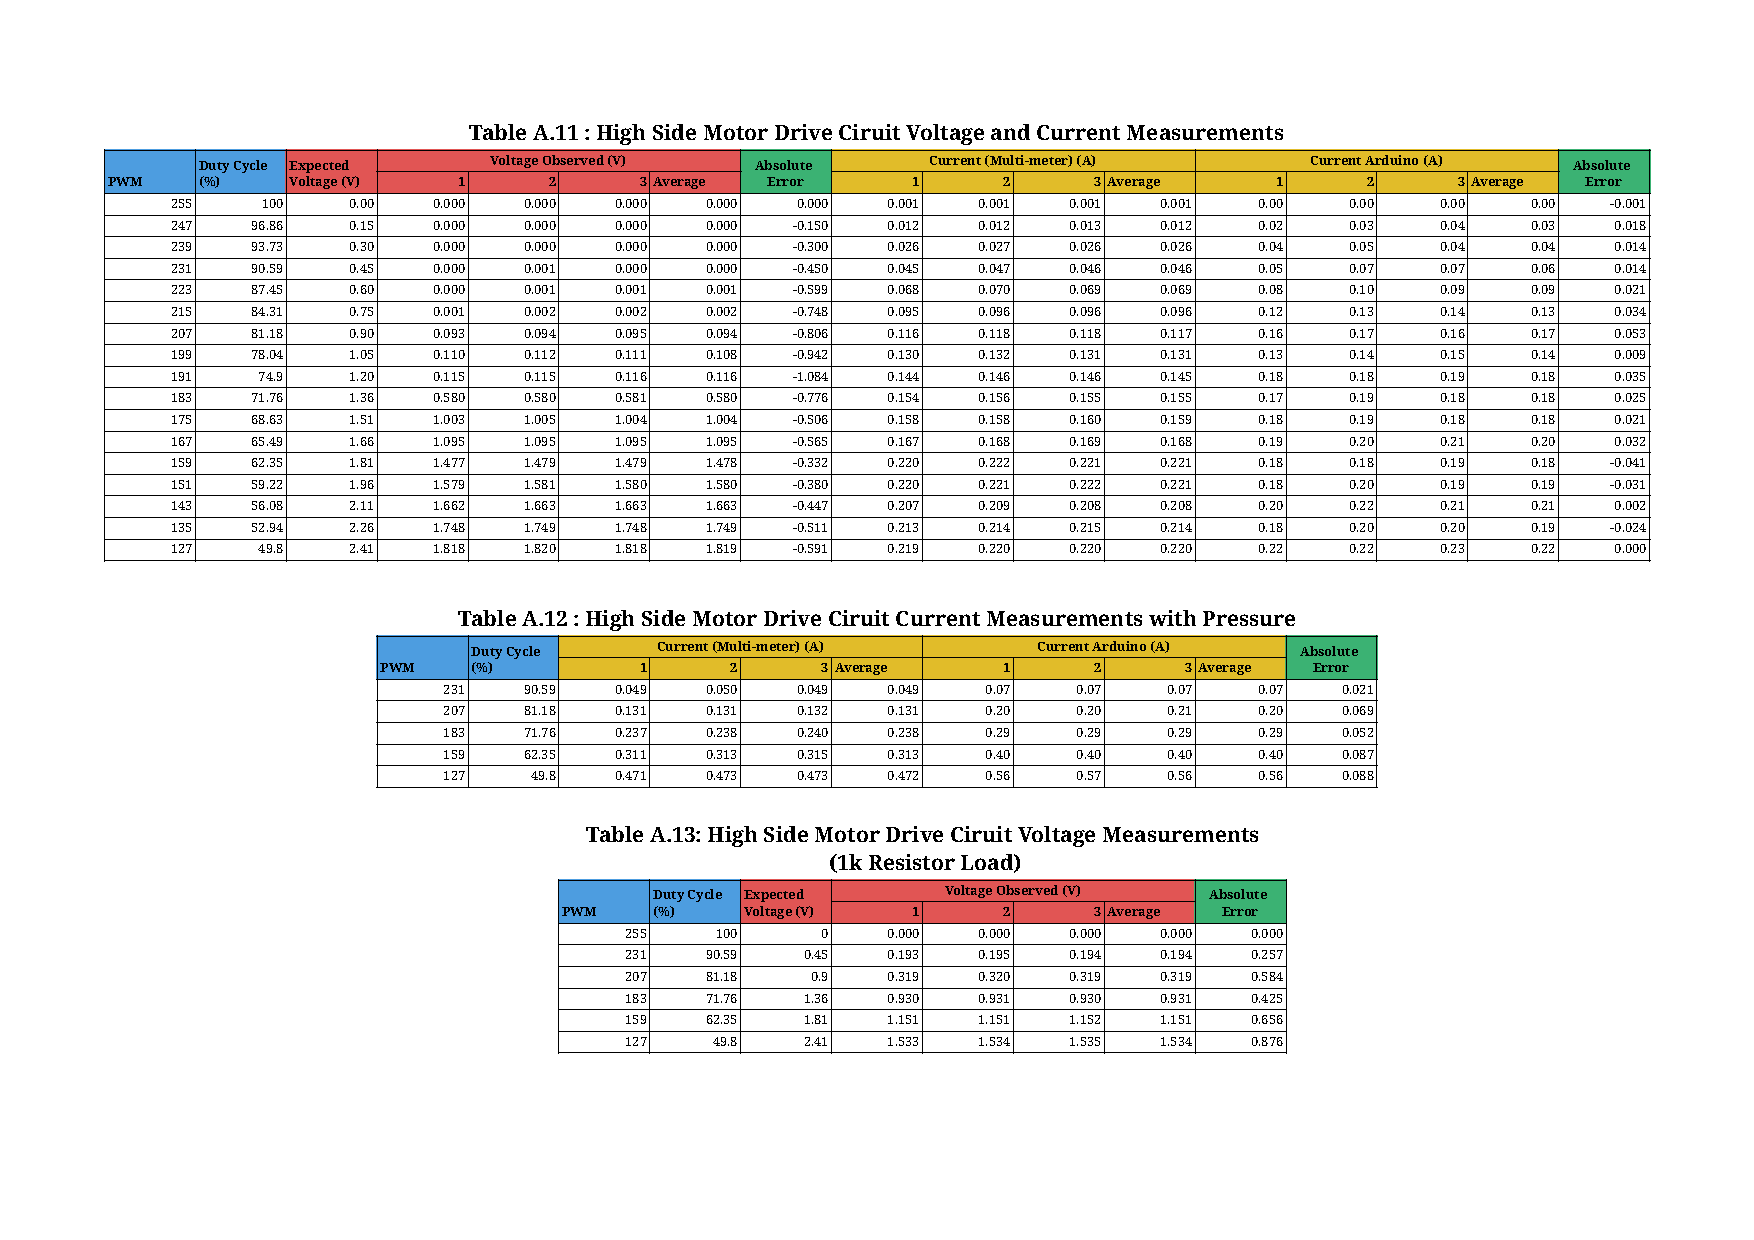
\includepdf[pages=-,landscape=true]{appendix data/Collation - HighSide.pdf}


\end{document}
